%==================================================================================================
%   LUKES THESIS TEMPLATE 1.2
%   -------------------------
%   This template is based upon the offcial IMM PhD Thesis template, it is enhanced with a number
%   of new features and a number of errors have fixed. This template is intended to be complied to
%   PDF using PDFLATEX and is tested using the MiKTeX 2.9 LaTeX distribution.
%   It is based on the official DTU-IMM Thesis template by Finn Kuno Christensen in 2009.
%   Small bugfixes by Kasper Laursen in 2012 and 2013.
%   Small updates by Finn Kuno Christensen/Henning Christiansen in 2015.
%   -------------------------
%   Last Updated: 2015-01-08
%==================================================================================================
%
%==================================================================================================
% DOCUMENT SETUP
%==================================================================================================
\documentclass[10pt,twoside]{book}                  %Official DTU-IMM Thesis document setup
%
%Set to 'print' for printed version, use 'net' for online version
%\def\thesisversion{print}
\def\thesesversion{net}
%
%==================================================================================================
% PACKAGES
%==================================================================================================
\usepackage{LukeThesis}                             %Import Thesis base style
%input{PhDMacros}                                   %Thesis specific macros
%

%==================================================================================================
% CUSTOM PACKAGES
%==================================================================================================
\usepackage{csquotes}
\usepackage[hyphenbreaks]{breakurl}
\usepackage{subcaption}
\usepackage{arrayjob}
\usepackage{tabularx}
\usepackage{ltablex} 
\keepXColumns
\usepackage{todo}
\usepackage{pifont}
\usepackage{longtable}
\usepackage{supertabular}
\usepackage{multirow}
\usepackage{enumitem} %% for effortless customization of enumeration
\usepackage{cleveref} %% for clever referencing
\usepackage{color}
\usepackage{transparent}
\usepackage[final]{pdfpages}
\usepackage{listings}
\def\UrlBreaks{\do\/\do-}
\usepackage[perpage,symbol*]{footmisc}
\usepackage{csvsimple}

\usepackage{macros}



%==================================================================================================
% MATH STUFFS
%==================================================================================================
\usepackage{mathtools}

\DeclarePairedDelimiter\ceil{\lceil}{\rceil}
\DeclarePairedDelimiter\floor{\lfloor}{\rfloor}


%==================================================================================================
% THESIS PROPERTIES (Modifiy these fields with your details)
%==================================================================================================
\def\thesisauthor{Daniel Schougaard}                     %Author
\def\thesistitle{Personal Password Manager in the Private Cloud}               %Title
\def\thesishandin{04-January}                       %Submission date (Day-Month}
\def\thesisdegree{M.Sc}                              %Degree ('B.Eng', 'B.Sc.', 'M.Sc.' or 'PhD')
\def\thesisyear{2015}                               %Submission year
\def\thesisnumber{????}                             %DTU-IMM Serial number (do not include year)
\def\thesisISSN{0000-0000}                          %ISSN number
\def\thesiskeywords{cloud, password, private, secure, encryption, privacy, keepass, lastpass}  %PDF keywords
\derivethesisprops                                  %Derive dependent properties
%
%==================================================================================================
% SECTION NUMBERING SETUP
%==================================================================================================
\setcounter{tocdepth}{2}                            %2 adds sections up to subsections
\setcounter{secnumdepth}{3}                         %Subsubsections get a number when this is 3
%
%==================================================================================================
% THESIS STRUCTURE  (Modifiy to include more chapters etc)
%==================================================================================================
\begin{document}
%------------------------
%Pre-frontmatter material
%------------------------
\prefrontmatter
%--------------------
%Frontmatter material
%--------------------
\frontmatter
\pagenumbering{roman}                               %Set frontmatter numbering style
\chapter{Summary (English)}
	In this thesis brief arguments as to why it is beneficial for individuals to host their own password manager, in a private-cloud. Having argued for this, a list of requirements for such an solution was devised. As a follow-up to these requirements, a thorough analysis was conducted. The analysis covered \emph{both} commercially available tools, \emph{and} theoretical academic solutions. The results were that no such solution exists, which adheres to every requirement, at this point in time.	As a consequence, a \emph{new} and improved design is proposed, adhering to \emph{all} of the requirements previously stated. Based on this extensive design, a prototype was implemented. Based on this prototype, rudimentary benchmarking was performed, to -- amongst others -- determine the viability of running the prototype on low-powered devices. Finally, the risks of using this prototype where discussed, and it was concluded that despite the inherent risks involved, it would still be beneficial to use the prototype.                                   %English summary of Thesis
\markboth{}{}                                       %Set headings (left)(right)
\chapter{Summary (English)}
	In this thesis brief arguments as to why it is beneficial for individuals to host their own password manager, in a private-cloud. Having argued for this, a list of requirements for such an solution was devised. As a follow-up to these requirements, a thorough analysis was conducted. The analysis covered \emph{both} commercially available tools, \emph{and} theoretical academic solutions. The results were that no such solution exists, which adheres to every requirement, at this point in time.	As a consequence, a \emph{new} and improved design is proposed, adhering to \emph{all} of the requirements previously stated. Based on this extensive design, a prototype was implemented. Based on this prototype, rudimentary benchmarking was performed, to -- amongst others -- determine the viability of running the prototype on low-powered devices. Finally, the risks of using this prototype where discussed, and it was concluded that despite the inherent risks involved, it would still be beneficial to use the prototype.                                   %Danish summary of Thesis
\markboth{}{}                                       %Set headings (left)(right)
\chapter{Preface}

This thesis was prepared at DTU Compute in fulfilment of the requirements for acquiring an M.Sc. in Engineering.

The thesis deals with ...

The thesis consists of ...
%==================================================================================================
% SIGNATURE AREA
%==================================================================================================
\vspace{20mm}
\begin{center}
    \hspace{20mm} Lyngby, \thesishandin-\thesisyear
    \vspace{5mm}
    \newline
  %Update signature image file in line below
    
\includegraphics[scale=0.5]{figures/SignatureDummy}
\end{center}
\begin{flushright}
    \thesisauthor
\end{flushright}
% % % EOF % % %                                     %Preface
\markboth{}{}                                       %Set headings (left)(right)
\chapter{Acknowledgements}

I would like to thank my....

                            %Acknowledgements
\markboth{}{}                                       %Set headings (left)(right)
%------------------
% Table of contents
%------------------
\newpage\mbox{}\newpage
\chaptermark{Contents}
\pdfbookmark{\contentsname}{toc}
\renewcommand{\sectionmark}[1]{\markright{#1}}
\sectionmark{Contents}
\addtolength{\parskip}{-\baselineskip}
\tableofcontents
\addtolength{\parskip}{\baselineskip}
\renewcommand{\sectionmark}[1]{\markright{\thesection\ #1}}
%-------------
% Main content
%-------------
\mainmatter
\chapter{Introduction}
\label{chap:intro}
	For many years, IT professionals have preached the importance of strong passwords. Many publications exist, describing exactly what defines a strong password. The general consensus is that it needs \emph{at least} both upper- and lower-case letters, digits and preferably also symbols \emph{(\#, \_, etc.)}. Additionally, it shouldn't be a word -- or a word where an L is replaced by a 1. And of course it has to be at least 8 characters long. And you're not supposed to use the same password more than once place. With all of these rules for strong passwords, it is hardly a surprise that a lot of the regular users of IT systems resort to simple and repetitive passwords.

	To help alleviate this problem, a new class of software grew popular: Password managers. Simple tools, protected by a single master password, which generate and store passwords in a secure manner. A lot of the IT professionals took these tools to their heart, despite their inherent flaws. 

	As with so many other things in modern society, the users crave convenience. Tools storing an encrypted file locally, was no longer sufficient, as the majority of users began to use multiple devices. Hence, the password managers slowly migrated into The Cloud.

	\section{The Cloud}
		The origin of the term ``The Cloud'' stems from Cloud Computing. Computations too heavy to be performed on a single machine, were divided onto several -- usually networked -- machines, which then shared the computational load. However, when we say the cloud today, it is not \emph{exactly} this we think of.

		The concept of the cloud is simple: Your data, and any computations associated with it, is stored and performed somewhere \emph{else}: In the so called cloud.

		This saves the users from the hassle of managing this, themselves. Applications such as Dropbox, OneDrive and Google Drive is prime examples of what the cloud exactly is: You unload some of the ``responsibilities'' onto something, or someone else. Once that file has been dragged into your Dropbox folder, and that little icon is green instead of blue, you're safe. Your data is now kept for you, available at all times, from any device. It is in the cloud.

		While the cloud \emph{does} come with its benefits, especially convenience, it has its own drawbacks as well. Let us talk about \emph{trust}.

		\subsection*{Trust}
			When uploading data into the cloud, the user is effectively trusting the vendor. They're trusting that the vendor is completely honest regarding their inner workings, what they can access and what they can not access. They are trusting the vendor, when they say that they do not \emph{(or possibly do)} sell your information to a third party.

			Trusting vendors is completely fine. You can't access the web without a certain amount of trust. Just look at the worlds most popular search engine, Google. Unfortunately, sometimes this trust is betrayed.

			Dropbox experienced this, when users discovered that the data they uploaded to Dropbox, was in fact not so private. Using hashing techniques to discover duplicate files, they ``save'' the user's bandwidth, by using an already stored file on their server. While this does sound like a reasonable feature, it also means that Dropbox has access to the raw files on their server somehow, which again leads us to question the privacy of Dropbox.

			Another example of this misplaced trust, is the incident involving LastPass in 2015. As many IT professionals had feared, the online password manager had a breach. Panic arose and LastPass almost forced their users to change their passwords. Exactly this, is the general issue with the cloud. You have to trust someone else to store it.

			This is the general issue with the cloud: You trust someone else to store your confidential information. Someone else to ensure that your data does not end up in the hand of someone else.

	\section{The Private Cloud}
		To counteract these issues, more and more people started hosting \emph{(self-hosted)} applications themselves, giving them cloud-like features, without ever relinquishing control or ownership of their data. This concept has evolved, especially during the last few years, into something called the ``private cloud''. 

		While the private cloud originally was intended for the various corporations and enterprise solutions, more and more open-source solutions have started to emerge. These solutions target users, tired of having to practically sign over ownership of their data, to benefit from seamless multi-device integration. They aim to create functionality, previously limited to the public cloud, by \emph{only} using the user's own hardware.

		Unfortunately, running a private cloud come with its own set of issues. First and foremost there is the issue of finances: A server not only costs money to acquire, but also to run. To run a server 24/7, would cost a fair amount. Secondly, there's the issue of setting this private cloud up. 

		\subsection*{The Financial Cost of the Private Cloud}
			\label{sec:privatecloud_cost}
			Previously, it was only enthusiasts with their own private \emph{servers} who was able to host these applications. These servers could be made from anything between an old discarded PC, to top of the line server hardware which the enthusiasts chose to buy. Unfortunately hardware like this, does have decently large power consumption, and if the user wants 100\% availability it needs to run 24/7.

			This trend however, has been changed a bit recently. With the rise of low powered computers, such as the Raspberry Pi, the Beaglebone, or even the Intel NUC, having a 100\% uptime no longer comes with an equally high cost. Using as little as $2.5W$, depending on the model. While this won't take the place of an ``actual'' server, it will be sufficient to run a single cloud-like application, creating a -- cheap to both acquire and run -- private cloud.

			Determining exactly how many $kWh$ such a device will consume -- over a year -- is quite easy. One simply have to fill out form \ref{eq:kwh} to calculate the total consumption of a device. If no rating of $W$ is given, it can be calculated, cf. equation \ref{eq:w}.

			\begin{equation}
				kWh_{year} = W_{device} \times h_{year} / 1000
				\label{eq:kwh}
			\end{equation}

			\begin{equation}
				W = V \times A
				\label{eq:w}
			\end{equation}

			Using a Raspberry Pi as the reference, an example value can be calculated. The Raspberry Pi Foundation has been generous enough, to post power consumption figures of their models online \cite{raspberrypi_power}. The newest -- and arguably most powerful -- model is the Pi3 B. They note it as having a \emph{maximum} power consumption of $1.34A$. Using this figure as an upper bound, the annual power consumption can be calculated, cf. \ref{eq:rpi_2_b_kwh}.



			%Since the Raspberry Pi Foundation has been so kind, as to provide a little table showing us the power consumptions of the different versions of the Raspberry Pi \cite{raspberrypi_power}, we can easily calculate the maximum theoretical consumption of a Raspberry Pi 2 B, which is the most powerful Rasberry Pi listed on the page.
			%shown on equation \ref{eq:rpi_2_b_kwh}.

			\begin{equation}
				kWh_{year} = (1.34A \times 5V ) \times 365.25 \times 24 / 1000 = 58.7322kWh
				\label{eq:rpi_2_b_kwh}
			\end{equation}

			%\todo{Wrong values used.}
			
			%Take note, that these values are for both the older models and the \emph{newest} model of the Raspberry Pi. Unfortunately the newest model only has a \emph{maximum} power drain noted, since it is recently new. 

			%The Model B+ from the previous generation, has the same maximum power drain, but it also have a significantly lower average power drain, of $0.33A$. They describe this drain, as caused by:
			%\begin{quote}
			%	\emph{Typical bare-board active current consumption.}\cite{raspberrypi_power}
			%\end{quote}

			However, this value represents the \emph{maximum} draw. In real world applications it is highly unlikely that it would be consuming that amount of power 24/7. Most of the time, the device would be idle, and in this state the Pi3B only uses $0.30A$. Using $0.50A$ as a more reasonable middle ground, the energy consumption for a year is reduced \emph{drastically}, to a mere $21.92kWh$, using equation \ref{eq:kwh}. 

			Taking prices of October 2015, a single kWh costs $2.22DKK$ \cite{energi_price} -- all inclusive. As such, it would cost around $50DKK$ to run a Rasberry Pi 3 Model B, 24/7 in Denmark. This leads to the conclusion that the cost is no longer a cause for only enthusiast and system administrators, to run their own private cloud. However, the cost is not the only issue in regards to running a private cloud.


		\subsection*{Technical Challenges}
			Unfortunately, the private cloud does not come without its own disadvantages. When using a vendor's solution, problems such as setup, configuration, and maintenance is their responsibility. Running an enterprise-like RAID environment will more than likely be out of the question, so taking precautions for data loss is definitely a priority.

	\section{The Problem}
		\label{chap:intro_sec:problem}
		The problem is passwords. There are two primary scenarios. One, they're too easy to bruteforce or simply guess, using social engineering. Or two, they're so difficult to remember that the user inadvertently returns to using the same password, over and over again, simply because of having to remember too many passwords. 

		Additionally, choosing the paranoid path, the passwords can \emph{not} be stored on a device not controlled by the user. This is mainly due to recent concerns regarding privacy of public hosts, such as LastPass.

	\section{Requirements}
		\label{sec:requirements}
		The requirements in the following sections are the requirements for the solution as a \emph{whole} and will therefore be independent of which technical structure is selected, during the design-phase.



		\subsection*{Functional Requirements}
			The most central requirement of the solution, is that it should \emph{not} be limited to a single device. It should be accessible from multiple devices, creating the feel of a private cloud. 

			The solution should support multiple \emph{(individual)} users, where a user can be either an admin user or a regular user. Passwords should be able to be organized in a structured way, customizable by the individual users, for the best user experience. For convenience, passwords should be able to be shared. However, sharing of passwords should not be the default setting, but something the user \emph{actively} have to select.

			The solution should be platform agnostic, and should not be limited to any \emph{one} server software. The solution has to be database agnostic, in such a way that the user can choose what type of underlying storage, he or she wishes. This is done to make it appealing to more hardcore enthusiasts as well, while also making it able to run on low powered devices. Access to the solution should be protected by the users master password, and using two-factor authentication should be a possible option. In order to better restrict outside access, the admin will have to create a new user. This can be done either with the admin actually setting up the user, or an invite to registration.

			No password -- or any other sensitive data -- should \emph{ever} be present unencrypted anywhere else, than a local device. This ensures that even if another part of the solution is somehow compromised, data is not revealed on that device.  The users should be able to audit access to their personal data including, but not limited to, retrieving passwords, adding passwords, changing passwords, and deleting passwords. This should be done by logging complete time of access and the remote host, at least. This ensures that a user can detect if unauthorised access has occurred.

			To sum it up, the above requirements have been condensed into a list:
			\vspace{-3ex}\begin{enumerate}
				\setlength\itemsep{0.1em}
				\item Distributed password database \label{requirement:distrib_password}
				\item Multi-user support \label{requirement:multi_user}
				\item Support differentiating between admin users and regular users. \label{requirement:admin_user}
				\item Password organisation, multiple levels \label{requirement:organization}
				\item Password sharing \label{requirement:sharing}
				\item Only admin can add a user -- or invite a user -- to the solution \label{requirement:add}
				\item Platform agnostic \label{requirement:platform}
				\item Database agnostic \label{requirement:database}
				\item Passwords and private information should never be stored or handled unencrypted anywhere, other than the local device. \label{requirement:passwords_local}
				\item Support adding of new passwords \label{requirement:new}
				\item Support retrieving stored passwords \label{requirement:retrieve}
				\item Support deleting stored passwords \label{requirement:delete}
				\item Extensive auditing \label{requirement:audit}
				\item Allow user authentication based on a single master password, per user \label{requirement:auth}
				\item Allow the user to change his or her master password \label{requirement:change}
				\item Support two-factor authentication \label{requirement:two-factor}
				\item Automatic start after a hardware reboot \label{requirement:restart}
			\end{enumerate}


		\subsection*{Non-Functional Requirements}
			Based on the previous sections, we can conclude one very fundamental thing: The passwords need to be stored somewhere the user has control over. In order to aid development, allowing for use of various open source frameworks and libraries, the solution should be open source and licensed with an appropriate license \emph{(MIT for instance)}. The solution should be able to store a million password entries \emph{(1.000.000)}, spread across all users. The encryption used for the storage of sensitive data should be of industry standard, and should be viable for at least 5 years. The same goes for the encryption used for communication. For maximum security, the solution should \emph{only} accept and use TLS version 1.2 connections, with a limited cypher suite. For the best user experience, there must not be any latency in the user interface, exceeding $500ms$. Any longer, and the user will grow tired of using the software, because of its sluggish feel.

			To sum it up, the above requirements have been condensed into a list:
			\vspace{-3ex}\begin{enumerate}
				\setlength\itemsep{0.1em}
				\item Only use user-controlled storage \label{requirement:user_storage}
				\item Open Source License \emph{(MIT for instance)} \label{requirement:open-source}
				\item Support for \emph{at least} 100.000 password entries \label{requirement:entries}
				\item Use encryption for storage should be viable for at least 5 years \label{requirement:encryption}
				\item Use encryption for communication should be viable for at least 5 years \label{requirement:comms}
				\item Secure communications, using only TLS 1.2 or newer \label{requirement:tls1.2}
				\item A user should never wait more than maximum $500ms$ after any action in the user interface, before the changes take effect \label{requirement:delay}
			\end{enumerate}




	\section{Contributions of the Project}
		Analysis
		Design
		Prototype described in Implementation

	\section{Structure of the Thesis}
\chapter{Analysis}
\label{chap:analysis}
	As is to be expected, solutions for solving the problem already exist. In this chapter these solutions are investigated and evaluated, as to how well they solve the problem at hand. While finding solutions that match the problem described in  \emph{completely} might be difficult, solutions that are fairly similar are also considered.

	Furthermore, available academic research papers will be studied, for solutions that would solve a problem similar to that in \ref{chap:intro_sec:problem}, or a interesting techniques for handling sub-problems.

	\section{Existing Available Tools}
		Having several available tools which -- more or less -- \emph{could} be used to solve the problems, the findings have been condensed into the following list.
		\begin{itemize}
			\item In-Browser Password Managers
			\item LastPass, and Similar Solutions
			\item KeePass, and Similar Solutions
			\item Rattic
			\item Encryptr
			\item Passwordstate
			\item Vault \emph{(Zoho)}
			\item TeamPasswordManager
			\item Simple Safe
			\item PassWork
			\item SimpleVault
			\item RoboForm
			\item TeamPass 
			\item Vaultier
			%\item Vault (https://vaultproject.io/)
		\end{itemize}
		In the following sections the user experience or the usability of the solution might seem to be attacked often. While this might be true, one simple fact remains: If the solution is not user friendly, the users will not use it. If they do not use the solution, it is effectively worthless.

		\subsection*{In-Browser Password Managers}
			\label{subsec:in-browser}
			\todo{Write section about in-password managers}
			\todo{Missing browsers: Chrome, Firefox, Safari, IE, Opera}

			The most used password manager of all times, is probably the one available to all: The password manager which is built-in into the various browsers. This is a feature most major browsers have adopted: Chrome, FireFox, Internet Explorer \emph{(now known as Edge)}, Safari and Opera.

			While all of the previously mentioned browsers support syncing \emph{(Internet Explorer only supports this using Windows 8.0 or newer.)} the passwords between devices, it requires to upload the passwords to one of the corporations websites.

			Additionally it lacks at one very important aspect: It only works for websites accessed through that \emph{specific} type of browser, i.e. only available in Chrome browsers. Passwords for email addresses  \emph{(assuming non-webmail)} for instance, wont be able to be easily retrieved. Already at this point, using the built-in password manager can be dismissed, simply due to its use cases.

			In \cite{browser_saved} they review the different browsers' storage format for their respective password managers. Their primary concern is, that while the passwords might be encrypted, both Firefox and Opera stores the decryption key directly on disk. If an attacker gets hold of this file, all passwords are available to him or her. Chrome and Safari, however, use Window's built in functions, and encrypts the files using the user accounts password for encryption. They note Firefox and Opera as the only browsers supporting a Master Password, which is to be entered every time the user accesses a password stored, which adds a bit of more security. However, their analysis could very well be deprecated by now. The version of Chrome, for instance, they're using is $V21.0$, while the current newest version is $V47.0$. 

			While this solution might seem interesting to some users, it still leaves a lot to be desired in regards to the requirements defined earlier.


		\subsection*{LastPass, and Similar Solutions}
			\label{subsec:lastpass}
			In the name of usability services such as LastPass\footnote{https://lastpass.com/}, PassPack\footnote{https://www.passpack.com/}, DashLane\footnote{https://www.dashlane.com/}, and so many others grew popular, and it is easy to understand why. Enabling you to access your passwords from several devices, through native apps or the browser, it seemed like it was the perfect match of usability and security. To avoid too much repetition LastPass is picked as a representative of this group, simply due to it being the most well-known.

			If we start by looking at the technical details of LastPass, they quote themselves using 256-bit AES encryption, and applies PBKDF2, in order to make it as difficult as possible, to crack stored data. For maximum security, both encryption and decryption, is done client side\cite{lastpass_cleintsideencryption}, as to avoid transferring the actual password, unencrypted, to their servers. Encryption and decryption is done using the master password, which is never actually sent to their servers. Finally, as is to be expected, all connections to LastPass' servers, are SSL encrypted.

			Having examined the technical aspect, we need to pay attention to the usability as well. Looking at their web UI, it shows a reasonably straight forward design. Allowing the user to organise passwords folders, creating a two-level structure, as seen on figure \ref{fig:lastpass_main} on page \pageref{fig:lastpass_main}. While this \emph{does} allow the user some level of organisation, several levels would have been preferable. Additionally, LastPass is renowned for their apps and plugins, covering all major operating systems and browsers, creating a near seamless integration, when it comes to addition of new passwords and auto-filling stored passwords.

			For devices without a browser supporting plugins, LastPass offers a so-called bookmarklet\cite{lastpass_bookmarklet}. A bookmarklet is a bookmark, which essentially contains JavaScript code, in order to add previously unobtainable features, in a browser. While this on the surface seems like a nifty feature, several studies have shown that the bookmarklets represent a significant security threat. In \cite{bookmarklet} they discuss an attack on LastPass, exploiting the users bookmarklet, to gain access to virtually all of the users stored credentials.

			However, with the recent leak from LastPass \cite{lastpass_leak}, more and more users grew suspicious of these services. No matter how much encryption you apply, you can not get around the fact, that you have to \emph{trust} LastPass to both be completely honest about their encryption technology, \emph{and} storing your sensitive data. In many of the more sceptical user's eyes, this is a huge drawback, and why this solution is deemed unusable to solve the problem at hand.


			\begin{figure}[h!]
				\centering
				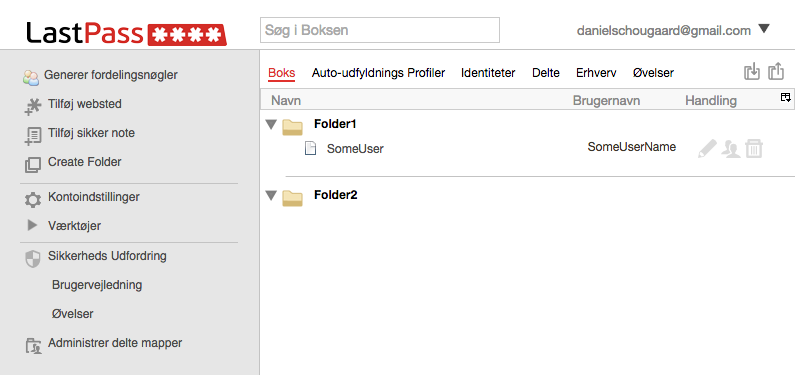
\includegraphics[width=\textwidth]{figures/analysis/lastpass_main.png}
				\caption{Screenshot of LastPass' main view, in a browser.}
				\label{fig:lastpass_main}
			\end{figure}

		\subsection*{KeePass}
			As the users grew suspicious of LastPass and the likes, a lot of them moved over to e.g. KeePass\footnote{https://keepass.org}, which allows the user to store the passwords in a local file. While there exists a plethora of tools similar to KeePass,  it will be used as a representative of this group, for the same reasons as in \ref{subsec:lastpass}.

			If we again start by examining the technical details, as of version 2.x KeePass only -- per default -- offers AES-256 encryption, which is seen on figure \ref{fig:keepass_create_security} on page \pageref{fig:keepass_create_security}, with additional algorithm choices available through plugins \cite{keepass_security}. This enables users to tailor the encryption security, to their own needs -- and beliefs. 

			Looking at the main UI, of which an example is shown on figure \ref{fig:keepass_main} on page \pageref{fig:keepass_main}, KeePass features exactly that which could be improved in LastPass: A tree like structure, in order to completely organise passwords. Other than that, there isn't anything noteworthy to say about their UI: It features the necessary and that's about it. A final thing worth mentioning, is that their password generator is completely customisable, as seen on figure \ref{fig:keepass_newpassword_passwordgen} on page \pageref{fig:keepass_newpassword_passwordgen}. You can manually choose, exactly which character sets, you wish to be in your passwords, enabling you to have passwords using local accents should the target system support it, which is a really nifty feature.


			However, having praised the features of KeePass, it does lack something extremely important: Usability. More precisely, it lacks distribution. Since KeePass works on a local file, it would only inherently work on a \emph{single} device. Should one wish to distribute it, another tool has to be involved. File synchronisation tools, such as Dropbox, Google Drive, or Syncthing could be used, in order to create a distributed-ish feel to KeePass. However, you do still rely on a third party tool, which is a drawback. Additionally, there is the lack of cross-platform compatibility, since \emph{officially} KeePass only supports Windows. Granted, there exists unofficial ports for Linux, OS X, Android, etc., but you have to trust the developers of these unofficial applications. By extension, this introduces the threat of security breaches. Another negative in regards to usability, is the lack of a browser extension. While there exists third party solutions for this, the authors personal experiences with setting these up and using them, is \emph{quite} negative.	

			Hence, all things taken into consideration, while KeePass has its moments it is an less than ideal solution.

			
			\begin{figure}[h!]
				\centering
				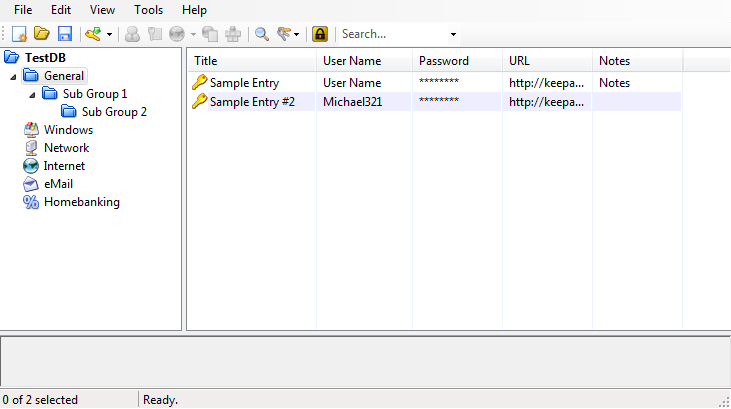
\includegraphics[width=\textwidth]{figures/analysis/keepass_mainview.png}
				\caption{Screenshot of KeePass' main view.}
				\label{fig:keepass_main}
			\end{figure}

			\begin{figure}[h!]
				\centering
				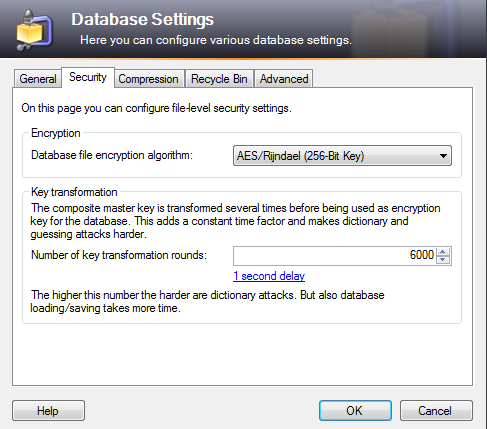
\includegraphics[width=0.7\textwidth]{figures/analysis/keepass_create_security.png}
				\caption{Screenshot of KeePass' security options.}
				\label{fig:keepass_create_security}
			\end{figure}
		
			%\begin{figure}[h!]
			%	\centering
			%	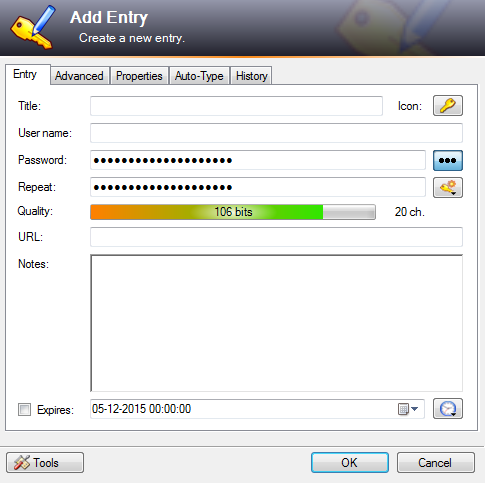
\includegraphics[width=\textwidth]{figures/analysis/keepass_newpassword_main.png}
			%	\caption{.}
			%	\label{fig:}
			%\end{figure}

			\begin{figure}[h!]
				\centering
				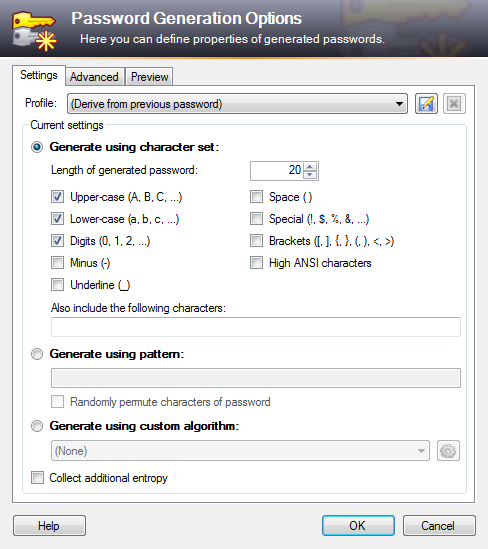
\includegraphics[width=0.7\textwidth]{figures/analysis/keepass_newpassword_passwordgen.png}
				\caption{Screenshot of KeePass' password generator settings.}
				\label{fig:keepass_newpassword_passwordgen}
			\end{figure}

		\subsection*{Rattic}
			Rattic\cite{rattic_frontpage} represents a third type of password manager, and the primary focus of this thesis: A self-hosted password manager, in the so-called private cloud. While at first glance, Rattic seems to be a solution very suited to the problem described earlier, it becomes a far more sketchy solution, upon investigating it closely. Rattic wonderfully describe their solution as:

			\begin{quote}
				\emph{RatticDB is a password management database designed for humans. We have focused on making it able to manage passwords for a team and to make that as easy as possible.}\\\cite{rattic_frontpage}
			\end{quote}

			Since Rattic \emph{is} meant for teams it has multi-user support. Rattic organises passwords and users in groups, and these groups are used for access control. A group is a collection of users, which can access the same passwords. An example of this could be \verb=DevelopmentTeam1= and \verb=DevelopmentTeam2=. Members of team one, can access their own passwords, and members of team two can access theirs, but unless specifically stated, they can not access each others. Additionally it supports tags for their passwords, allowing for even further organisation, for their users allowing quick access to similar passwords, from across different groups.

			However, the fact that Rattic markets itself at teams, rather than individual users is evident by the fact that as per default, you can not create ``private'' passwords, which only a single user can access. To achieve that, you would need to manually create a new group -- per user -- with only said user as member. While this would work, it is very much a work-around of Rattic's default behaviour, for it to work that way.

			From a user experience point of view, Rattic is a rather friendly tool. On figure \ref{fig:rattic_main} on page \pageref{fig:rattic_main}, you see a clean, minimalistic view of available passwords. Granted, this figure is from an Admin's point of view, hence he can access both the \verb=DevelopmentTeam1= and \verb=DevelopmentTeam2= groups, and consequently passwords stored under them.

			\begin{figure}[h!]
				\centering
				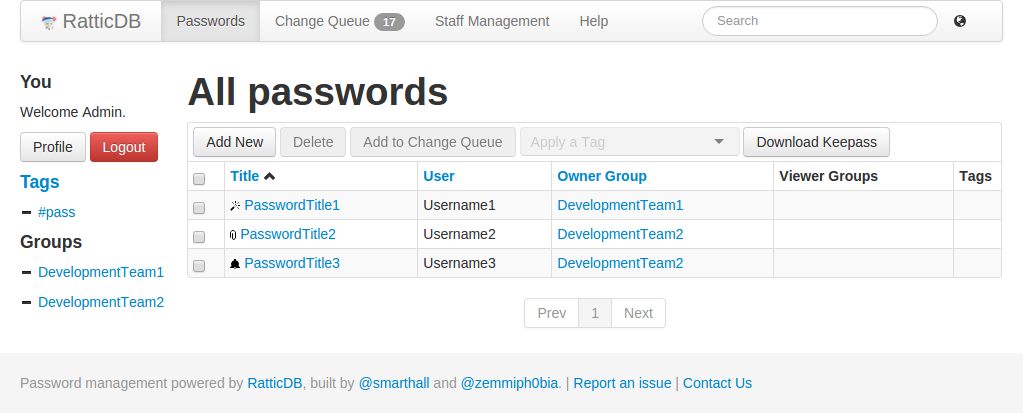
\includegraphics[width=0.95\textwidth]{figures/analysis/rattic_main.png}
				\caption{Rattic's Frontpage of their Web UI.}
				\label{fig:rattic_main}
			\end{figure}

			Adding passwords is just as easy in KeePass, cf. figure \ref{fig:rattic_newpassword_main} on page \pageref{fig:rattic_newpassword_main}. Simply type in the details, select an owner group and submit. While the password generator, cf. figure \ref{fig:rattic_newpassword_passwordgen} on page \pageref{fig:rattic_newpassword_passwordgen}, could stand to have some additional features, it is sufficient for generating strong passwords with high enough entropy. A nifty little feature, is the \verb=Download KeePass= button, which allows a user to download passwords in the KeePass format, making it available for later offline use.

			\begin{figure}[h!]
				\centering
				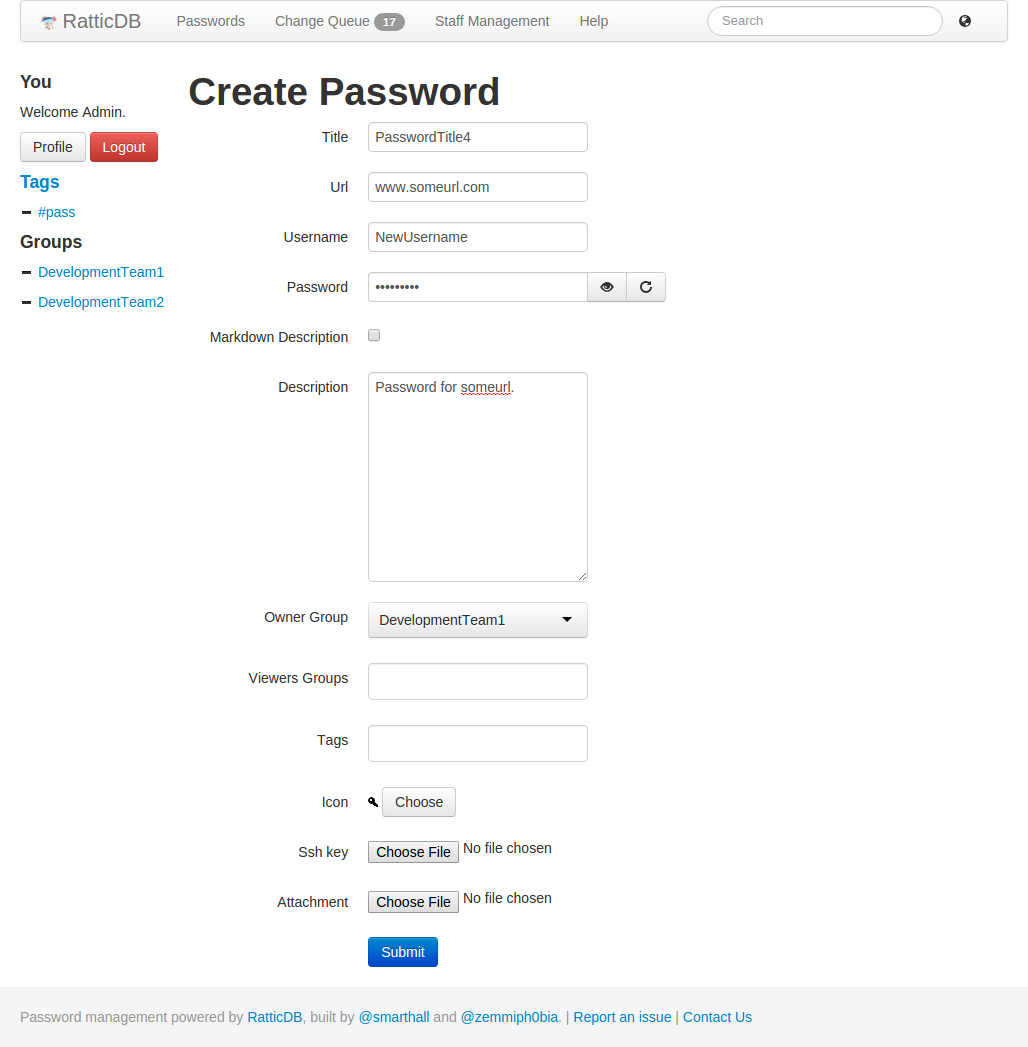
\includegraphics[width=0.95\textwidth]{figures/analysis/rattic_newpassword_main.png}
				\caption{Adding a new password, in Rattic.}
				\label{fig:rattic_newpassword_main}
			\end{figure}

			\begin{figure}[h!]
				\centering
				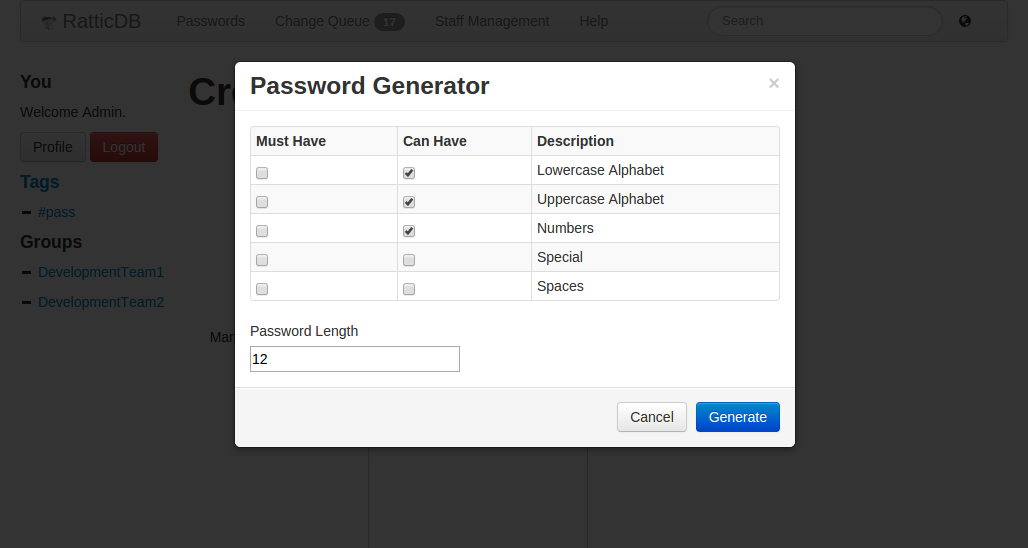
\includegraphics[width=0.95\textwidth]{figures/analysis/rattic_newpassword_passwordgen.png}
				\caption{Generating a password in Rattic.}
				\label{fig:rattic_newpassword_passwordgen}
			\end{figure}

			Having said that, there are some technical concerns, regarding Rattic. Rattic does \emph{not} encrypt passwords stored in the database -- something they are very open about. In \cite{rattic_encryption} they argue heavily for their lack of encryption, due to requiring less code and tests. They do, however, highly recommend storing the database on an encrypted drive, to ensure database protection. However, this \emph{does} mean that a sysadmin can access \emph{all} passwords, should he or she have the encryption key for the drive. Due to this, the deployment of Rattic is fairly complex, as they admit themselves. 

			Rattic is developed in Python, using the Django framework and tested on the Apache server.

		\subsection*{Encryptr}
			Bordering between the type of LastPass and Rattic, Enryptr \cite{encryptr} relies on the Crypton\cite{crypton} backend\cite{encryptr_backend}, available hosted at SpiderOak\cite{crypton_spideroak}. Per default, Encryptr \emph{only} supports hosting passwords at the Crypton backend, hosted at SpiderOak. However, it \emph{is} possible to run this in the private cloud, with your own Crypton backend. \emph{But} it requires manually editing source files\cite{encryptr_selfhost}, which makes the setup a pain. So not only would you have to set up Crypton, and its requirements, you would have to download the source of the apps, change the specified line of code, compile and \emph{then} you could use it. Because of this technical aspect, usability is virtually zero, as you would need to be fairly confident behind a keyboard, to successfully set this up.

			Having said that, the UI of Encryptr is \emph{very} minimalistic and sleek, which both is a good and a bad thing. As seen on figure \ref{fig:encryptr_main} on page \pageref{fig:encryptr_main}, all passwords are stored in a \emph{single} list: There is \emph{no} organisation, other than labels. Granted, they do support searching, but somehow that still makes it very confusing, if more than a handful of passwords or secrets are stored, and since Encryptr not only supports storing passwords, but also credit card information and general secrets, this could be achieved fairly quickly.

			Adding a passwords shows something disturbing: Lack of a decent password generator, cf. figure \ref{fig:encryptr_newpassword} on page \pageref{fig:encryptr_newpassword}. Once the form for adding a new password is opened, a password is generated as per some default behaviour. There is no customising entropy of the password, or even something as simple as the length.

			\begin{figure}[h!]
				\centering
				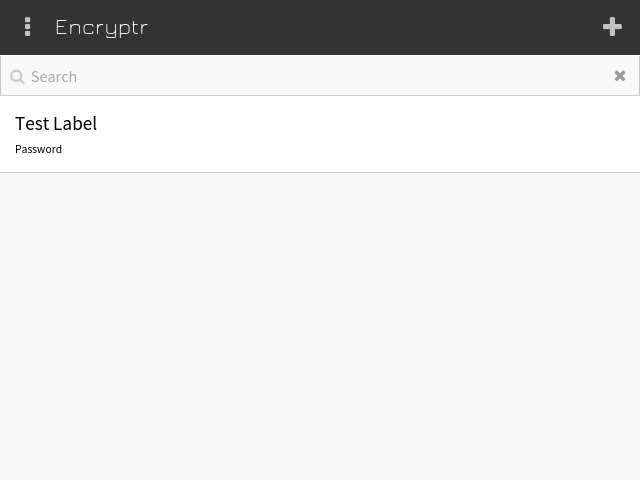
\includegraphics[width=0.75\textwidth]{figures/analysis/encryptr_main.png}
				\caption{Encryptr's main view.}
				\label{fig:encryptr_main}
			\end{figure}


			\begin{figure}[h!]
				\centering
				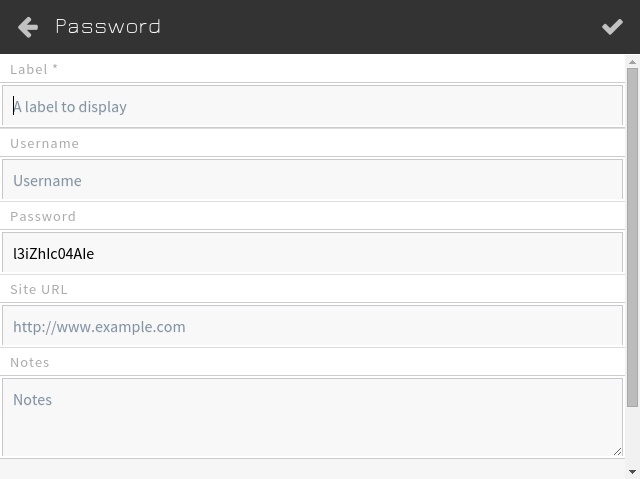
\includegraphics[width=0.75\textwidth]{figures/analysis/encryptr_newpassword_main.png}
				\caption{Adding a new password in Encryptr.}
				\label{fig:encryptr_newpassword}
			\end{figure}

			On the technical side, Crypton -- the backend -- is actually fairly interesting. Using their own definition of zero-knowledge, the developers created a complete framework for securely transferring and storing data at a remote machine\cite{crypton_paper}. They claim, that it is impossible to obtain the unencrypted data on their servers, without actually getting hold of the users private encryption key. The Crypton backend is open source, and available at \cite{crypton_git}. What powers Crypton, cryptographically speaking, is AES-256.

		\subsection*{Vault}
			Vault\emph{(ZOHO)}\cite{vault_zoho} is another piece of software, that requires you to submit your data to their servers. Where this tool differs from LastPass and Encryptr, is that it is \emph{clearly} aimed at enterprise customers, which is clearly evident based on their features, such as LDAP integration.

			Vault organises the passwords in so called Chambers. Each password \emph{can} be added to one or more chambers, but is not necessary. Seen on figure \ref{fig:vaultzoho_main_secrets} on page \pageref{fig:vaultzoho_main_secrets} we see how it lists all available passwords, in a single list. Using this main list quickly becomes very confusing. Looking at the Chambers list, which is found on figure \ref{fig:vaultzoho_main_chambers} on page \pageref{fig:vaultzoho_main_chambers}, the same pattern arises again. A large list, showing only the important information -- the passwords -- in the smallest part of the UI. All in all, performing simple tasks is very clunky.

			As with Encryptr, password generation lacks a lot. A password can be generated -- and re-generated -- but it happens after some under-the-hood-behaviour, which the user can not choose to customise.


			\begin{figure}[htbp]
				\centering
				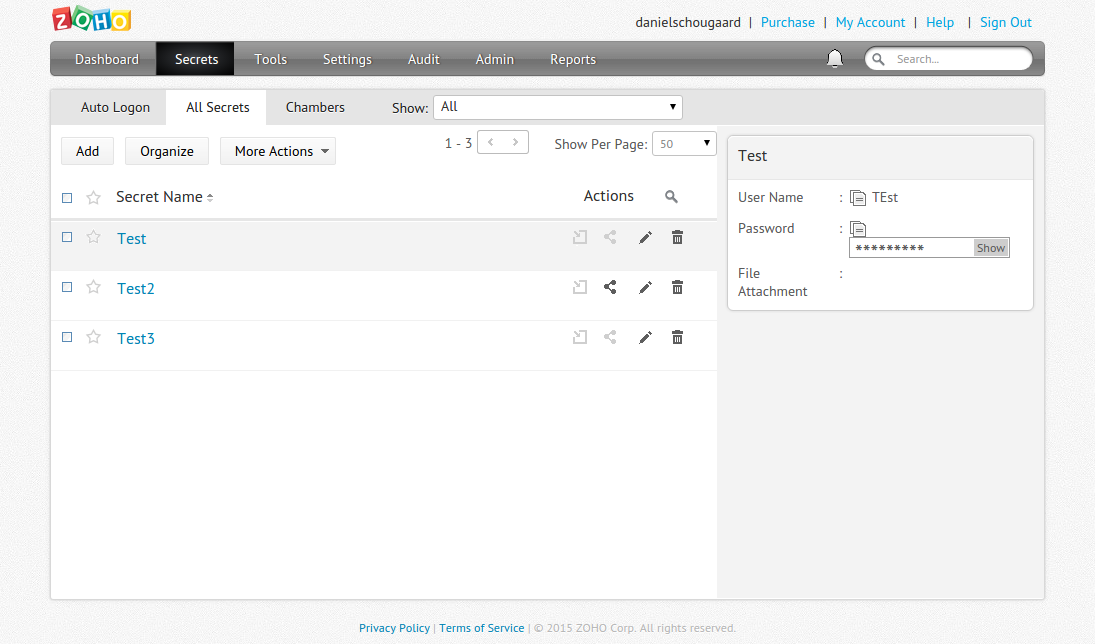
\includegraphics[width=0.95\textwidth]{figures/analysis/vaultzoho_main_secrets.png}
				\caption{Listing all stored secrets in Vault \emph{(ZOHO)}.}
				\label{fig:vaultzoho_main_secrets}
			\end{figure}

			\begin{figure}[htbp]
				\centering
				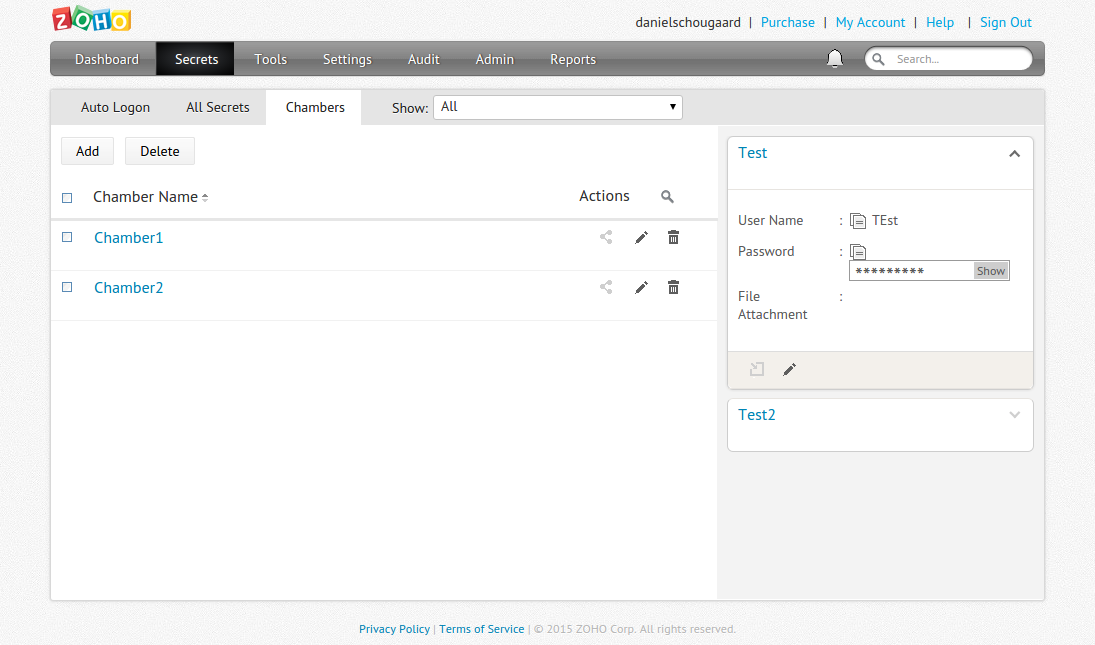
\includegraphics[width=0.95\textwidth]{figures/analysis/vaultzoho_main_chambers.png}
				\caption{Listing Chambers stored in Vault \emph{(ZOHO)}.}
				\label{fig:vaultzoho_main_chambers}
			\end{figure}


			Under the hood, Zoho uses a combination of RSA and AES. To enable sharing, a common AES encryption key is retrieved using RSA keypairs, from the admin, and users involved in sharing\cite{vault_zoho_encryption}.

		\subsection*{TeamPasswordManager}
			TeamPasswordManager\cite{teampasswordmanager_frontpage} \emph{(henceforth referred to as TPM)} is a tool that is fairly similar to Rattic. However, where it differs is the less minimalistic UI. TPM organises passwords in ``Projects'', which is a great indicator that this tool is in fact intended to be used with enterprise in mind. TMP is able to be self-hosted and is platform independent, requiring Apache, PHP and MySQL, which is a great asset.

			Turning to the user experience, the frontpage that the user is presented with, as seen in figure \ref{fig:teampasswordmanager_main} on page \pageref{fig:teampasswordmanager_main}, is a clunky list of all available passwords. For organisational value, groups as ``Favorite'' and ``Recent'' are also available, filtering the available passwords into more manageable lists. But once again, this very clunky and large UI is used, much like in Vault.

			TeamPasswordManager aims itself at -- as the name implies -- teams, much like Rattic. This choice, is very apparent in the work flow. For instance, a password is tied to a ``project", instead of a user. Where TPM excels, is the fact that a project can contain sub-projects, which in return can contain sub-projects, and so forth. This creates a tree-like structure, much like that of KeePass, which can be seen on figure \ref{fig:teampasswordmanager_tree} on page \pageref{fig:teampasswordmanager_tree}.


			\begin{figure}[htbp]
				\centering
				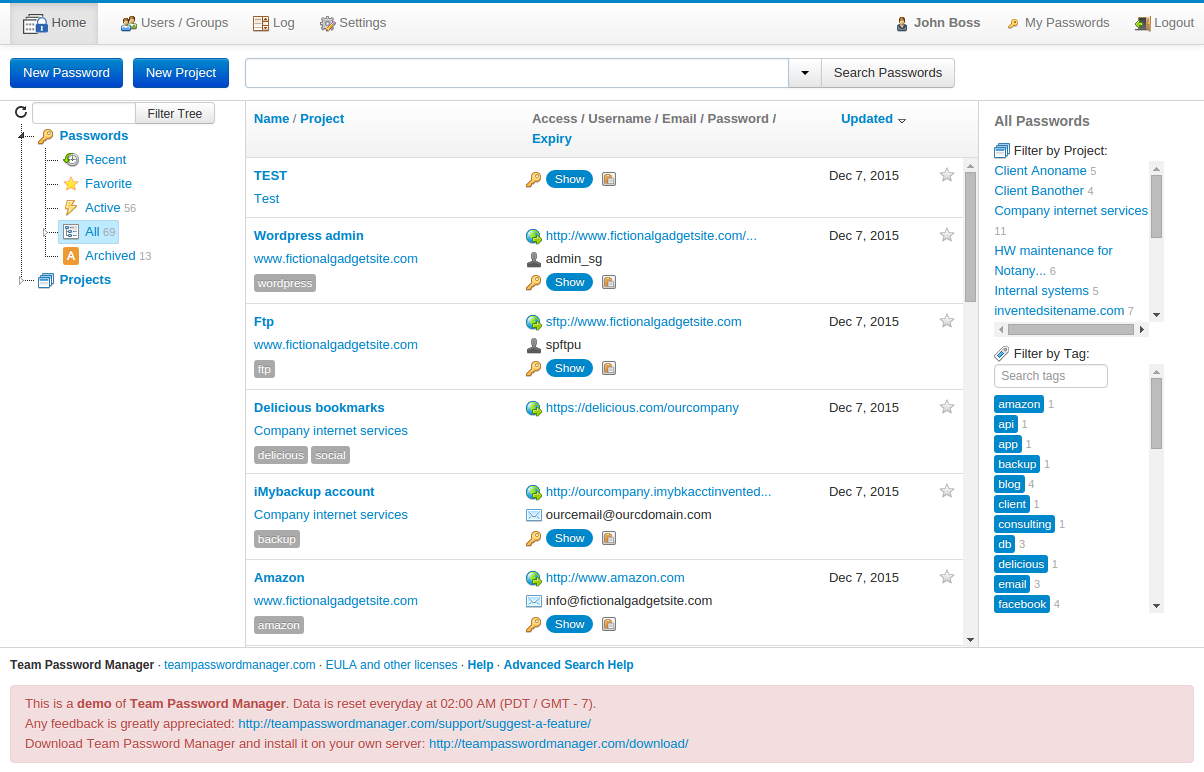
\includegraphics[width=0.95\textwidth]{figures/analysis/teampasswordmanager_main.png}
				\caption{Front page of TeamPasswordManager's web interface.}
				\label{fig:teampasswordmanager_main}
			\end{figure}

			\begin{figure}[htbp]
				\centering
				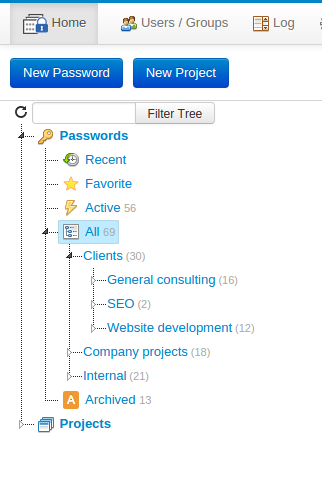
\includegraphics[width=0.35\textwidth]{figures/analysis/teampasswordmanager_tree.png}
				\caption{The tree-like organisational structure of TeamPasswordManager.}
				\label{fig:teampasswordmanager_tree}
			\end{figure}

			Encryption wise, TPM uses the same basic algorithm we've seen over and over again: AES-256. TPM also uses bcrypt as their chosen key derivation function, to make it as difficult for a potential attacker to brute force password hashes. Using Google's Authenticator, it supports two-factor authentication.

			While this software could essentially suffice, in order to meet the requirements, it would be lacking heavily in the user experience department. Additionally, it provides features and information, which would only be of use to super-users, and enterprise users, and might very well scare off regular users.

		\subsection*{Passwordstate}
			Passwordstate from ClickStudios\cite{passwordstate} is a solution some-what similar to both TeamPasswordManager and Vault \emph{(Zoho)}. There is not a seconds doubt, that this is a solution aimed at enterprise users, as they state themselves. This is also evident by the feature set, they have: Sporting not only active directory support, they also have built-in options for High Availability and \emph{several} options for two-factor authentication, amongst others. Passwordstate is self-hostable, but requires a windows platform and the IIS server \cite{passwordstate_requirements}.

			Inspecting the user experience, reveals that Passwordstate is a fresh breeze. This solutions actually manages to give the most important information, the most screen-space. On figure \ref{fig:passwordstate_main} on page \pageref{fig:passwordstate_main}, we see how password state allows for the same tree-like structure, that we've seen before. This creates excellent organisational options, for the users. On the frontpage the user is presented with his or hers favourite passwords list, and recently accessed passwords. Alas, here is where Passwordstate falls short. Instead of keeping a minimalistic UI, the user is presented with information, only interesting to enterprise users, or super-users. A host list, is with a high probability useless for the majority of regular users, as well as the little graph that shows password statistics, as seen on figure \ref{fig:passwordstate_graph} on page \pageref{fig:passwordstate_graph}. This particular graph, presented at this particular place, seems very much to be a graph for the sake of a graph. 

			Additionally, accessing passwords is not straight forward: Again, Passwordstate presents the user with a \emph{lot} of enterprise options, which is far from beneficial for a regular user. The available options can be seen on figure \ref{fig:passwordstate_getpassword} on page \pageref{fig:passwordstate_getpassword}. Taken all of these things into consideration, Passwordstate is an excellent password manager for enterprises, already running Windows as their server software. However, for regular home users, the software is simply \emph{far} too complex.

			Passwordstate has the options to completely customise the rules, that a password is generated by, much like KeePass. On figure \ref{fig:passwordstate_newpassword_passwordgen} on page \pageref{fig:passwordstate_newpassword_passwordgen} you see the \emph{extensive} options, enabling the user to customise the password to their needs.

			\begin{figure}[htbp]
				\centering
				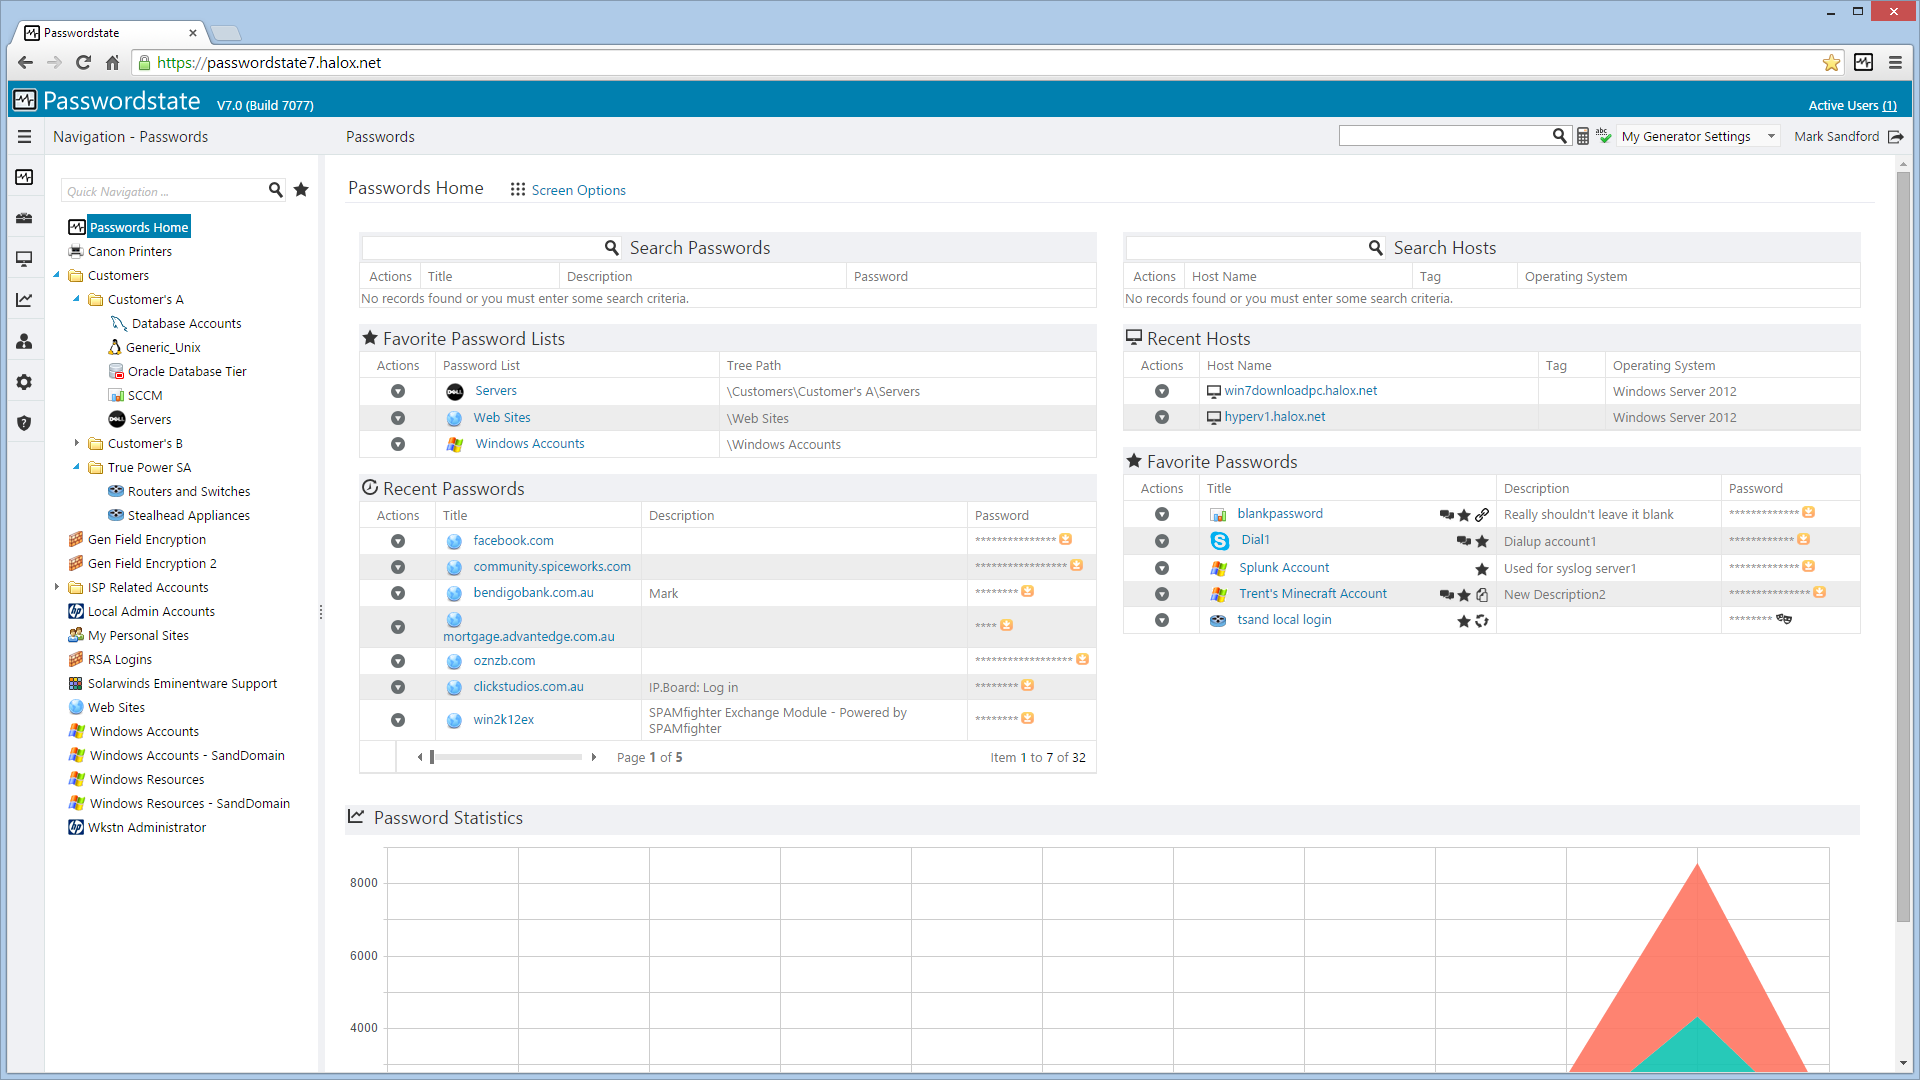
\includegraphics[width=0.95\textwidth]{figures/analysis/passwordstate_main.png}
				\caption{Frontpage of the PasswordState website. \figsrc{fig:passwordstate_main} }
				\label{fig:passwordstate_main}
			\end{figure}

			\begin{figure}[htbp]
				\centering
				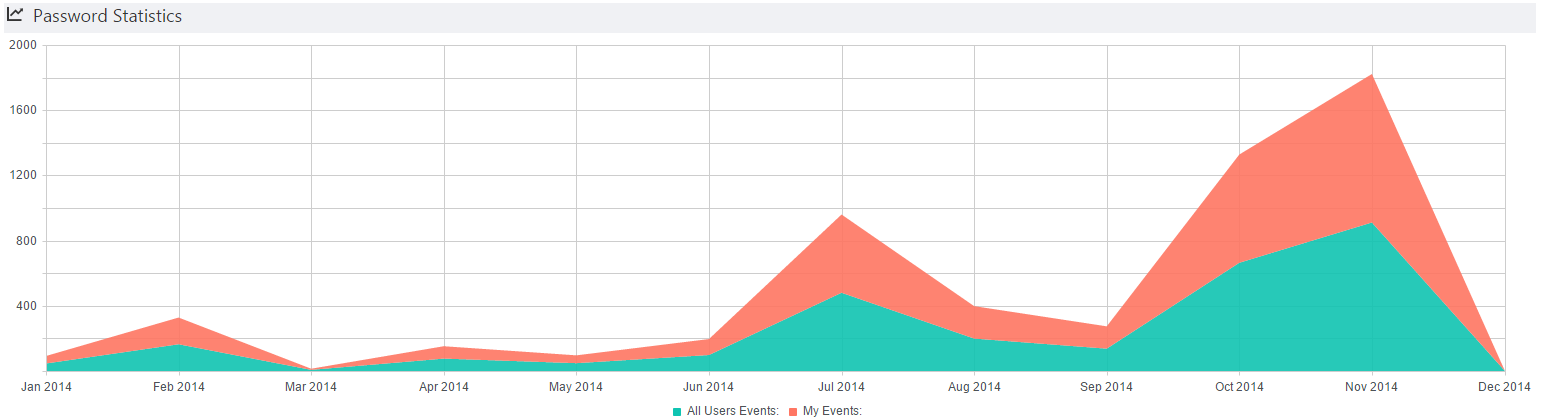
\includegraphics[width=0.95\textwidth]{figures/analysis/passwordstate_graph.png}
				\caption{Password statistics graph, in PasswordState. \figsrc{fig:passwordstate_getpassword}}
				\label{fig:passwordstate_graph}
			\end{figure}

			\begin{figure}[htbp]
				\centering
				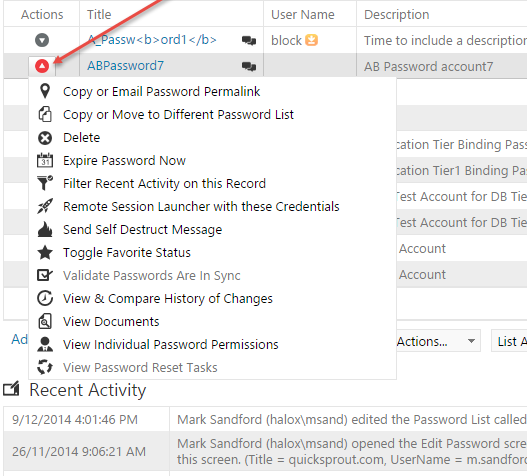
\includegraphics[width=0.7\textwidth]{figures/analysis/passwordstate_getpassword.png}
				\caption{Retrieving a password in PasswordState. \figsrc{fig:passwordstate_graph}}
				\label{fig:passwordstate_getpassword}
			\end{figure}

			\begin{figure}[htbp]
				\centering
				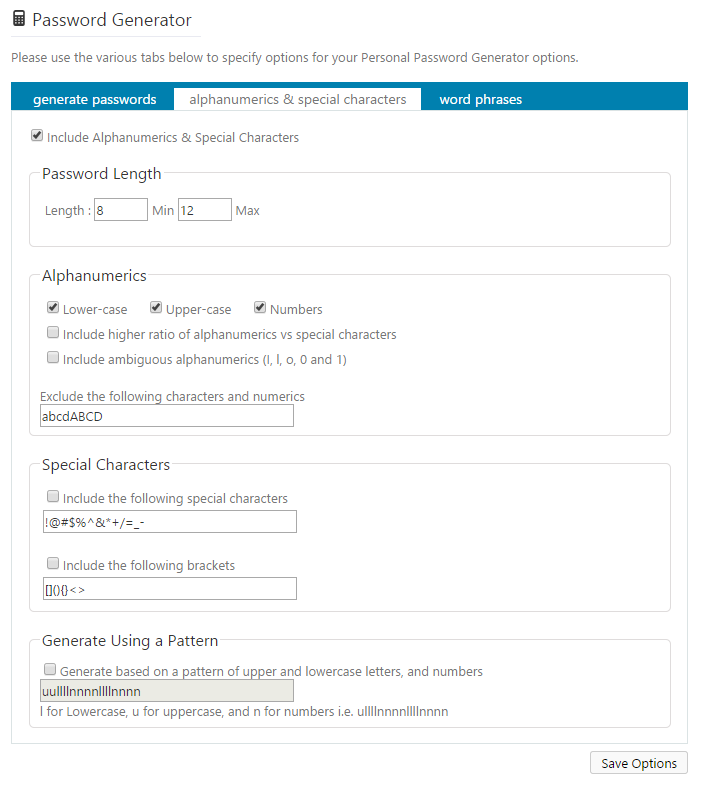
\includegraphics[width=0.95\textwidth]{figures/analysis/passwordstate_newpassword_passwordgen.png}
				\caption{Generating a new, secure, password in Passwordstate. \figsrc{fig:passwordstate_newpassword_passwordgen}}
				\label{fig:passwordstate_newpassword_passwordgen}
			\end{figure}

			Looking at the technical side, Passwordstate encrypts all passwords using AES-256\cite{passwordstate_security}, which seems to be the standard. Additionally, all sensitive information is salted. Passwordstate protects their sourcecode by the use of:
			\begin{quote}
				\emph{... precompiled ASP.NET pages and obfuscated .NET Assemblies. No longer can web or database administrators gain access to data they are not authorised to view. }\cite{passwordstate_security}
			\end{quote}

			Unfortunately, the limited number of platforms Passwordstate can run on, is a \emph{huge} drawback.

		\subsection*{SimpleSafe}
			SimpleSafe\cite{simplesafe} is another take on the self-hosted team password manager solution, which seems to be the predominant solution available. Unfortunately SimpleSafe's documentation is lacking heavily, but based on their available demo, it appears that all users have access to all passwords. This results in that a single user can not have a private password, for their use only.

			While it appears they have whole-heartedly embraced the idea of a minimalistic design, they've done so at the expense of user experience. The main view is a rather large but accessible list, with customizable attributes. On figure \ref{fig:simplesafe_main} on page \pageref{fig:simplesafe_main} the list is shown. The user can chose to organise passwords \emph{(or custom entries)} into groups. Groups are accessed through a menu, which is auto hidden. The expanded menu is shown on figure \ref{fig:simplesafe_menu} on page \pageref{fig:simplesafe_main}. Unfortunately, changing between groups takes a \emph{long} time. This causes a horrible experience for the user. Generally, the developers of SimpleSafe have been very generous with the animations, as pretty much all actions in the UI invokes some kind of animation. The delays because of this, adds to the overall sluggish feel of the system.

			\begin{figure}[htbp]
				\centering
				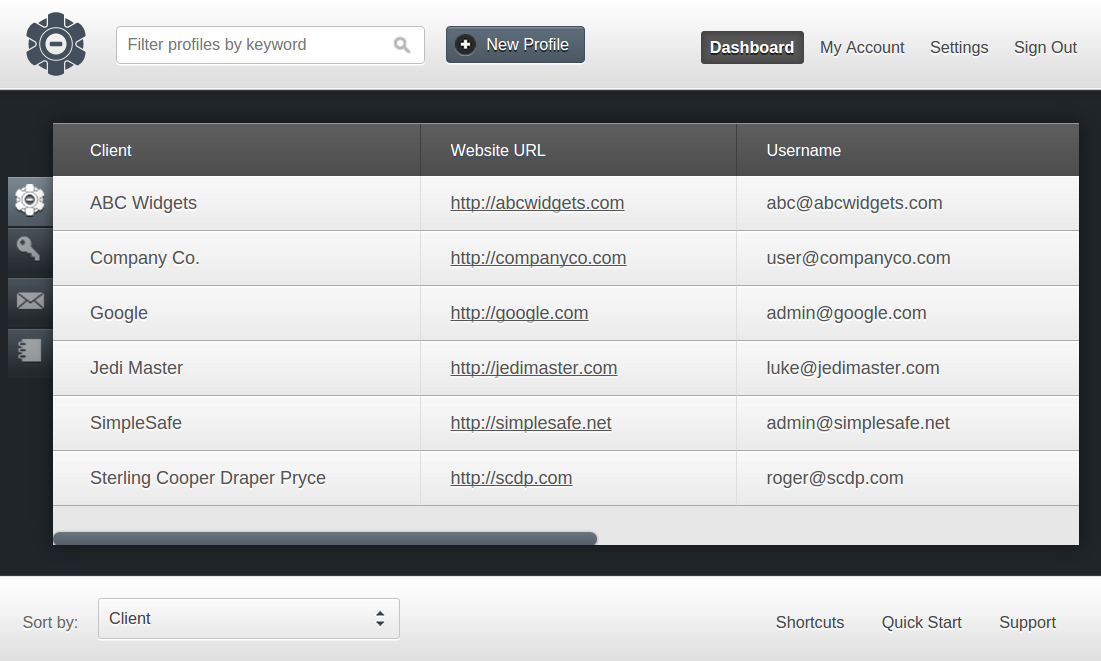
\includegraphics[width=0.95\textwidth]{figures/analysis/simplesafe_main.png}
				\caption{Homepage of SimpleSafe}
				\label{fig:simplesafe_main}
			\end{figure}

			\begin{figure}[htbp]
				\centering
				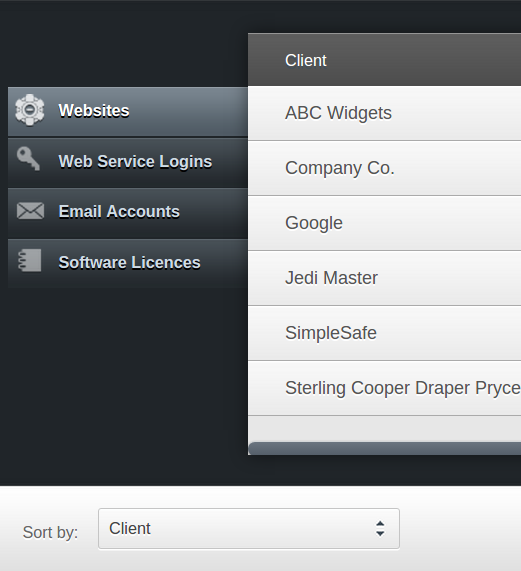
\includegraphics[width=0.70\textwidth]{figures/analysis/simplesafe_groups.png}
				\caption{Menu for changing groups in SimpleSafe.}
				\label{fig:simplesafe_menu}
			\end{figure}

			Security wise, it is \emph{very} difficult to inspect SimpleSafe, due to their own lack of description. The only available information regarding security or encryption is the following quote.
			\begin{quote}
				\emph{SimpleSafe utilises a 256 bit encryption method. Each password has a unique private salt along with a master salt stored separately to the database. Only encrypted passwords are stored within the database.}\cite{simplesafe_faq}
			\end{quote}

			All in all SimpleSafe is a \emph{fairly} sketchy solution. One thing that is pretty neat, is the ability for a user to customise the fields in the different groups. For instance, they allow you to store SSH keys, in a particular field type. This lets the user separate things that require keys / certs, from traditional username/password logins.

		\subsection*{PassWork}
			PassWork\cite{passwork} is yet another take, on the same type of solution as SimpleSafe, Rattic, TeamPasswordManager, and Passwordstate. PassWork is available as both a remote and a self-hosted solution, both of which comes with a price tag. 

			PassWork organises passwords in groups, which in return can contain sub-groups -- or folders as the icon resembles. Each group has a list of users, currently allowed to access passwords in said group. As figure \ref{fig:passwork_adduser} on page \pageref{fig:passwork_adduser} shows, users can be added to groups, with permissions ``Full Access'', ``Edit'', and ``Read''. While differentiating between ``Edit'' and ``Full Access'' might be difficult, the option of setting permissions \emph{that} easily, when adding a user, is surprisingly a very good feature. Per default a group called a ``My passwords'' group is created, in which the user can place private passwords. 

			\begin{figure}[htbp]
				\centering
				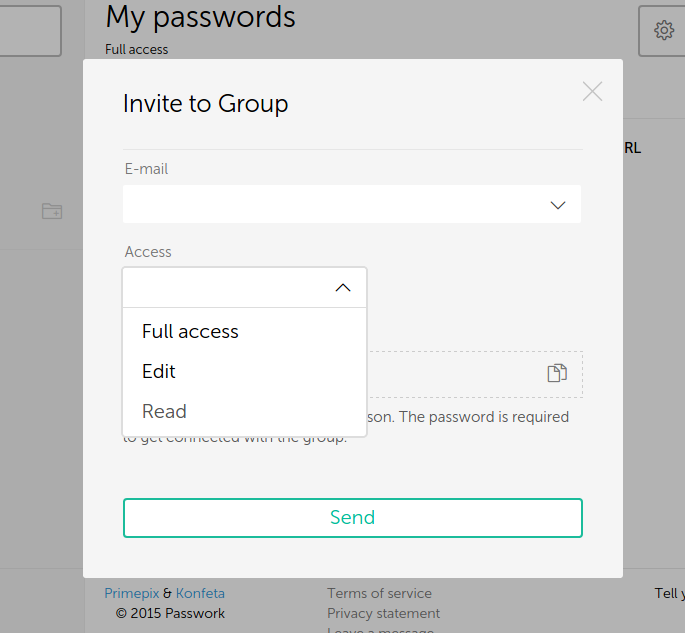
\includegraphics[width=0.95\textwidth]{figures/analysis/passwork_adduser_cropped.png}
				\caption{Permissions available, when adding users to a group.}
				\label{fig:passwork_adduser}
			\end{figure}

			PassWork is another example of developers not describing and documenting their soltion properly. Something as simple as figuring out which platform it supports, prior to purchasing is not possible. Additionally it is impossible to completely determine their encryption scheme, but they use ``256-bit passwords'' and RSA keypairs for sharing passwords. 

			Their less than completely transparency when it comes to choice of encryption algorithm not to mention the hefty price-tag, should one wish to self-host it. Additionally, they completely omit to inform which platform(s) the self-hosted version is able to be run on.

		\subsection*{SimpleVault}
			Taking a bit of a different route from other solutions, SimpleVault\cite{simplevault} chooses to encrypt each individual password, with a different ``passphrase''. Based on their user experience, it would seem that SimpleVault is a proof of concept, more than a release software. Something as simple as headers for the table containing the main information is missing, as seen on figure \ref{fig:simplevault_main} on page \pageref{fig:simplevault_main}.

			Adding a password, on figure \ref{fig:simplevault_addpassword}, shows the same lack of attention to the user experience, having two fields completely undescribed. One thing that SimpleVault \emph{does} get right in this context, is the option to generate passwords. Three buttons exists for generating passwords, with increasinly ``rare'' symbols. While options for passwords of specific length lacks, it seems to -- per default -- generate password of suitable length. 

			Retrieving a password, on figure \ref{fig:simplevault_getpassword}, requires the user to type in the passphrase. The choice of this per-password passphrase, will undoubtedly only result in the user using the same password over and over again. However, this choice \emph{does} allow for the system to be used by multiple users, each just using their own master passphrase for all of their passwords.

			\begin{figure}[htbp]
				\centering
				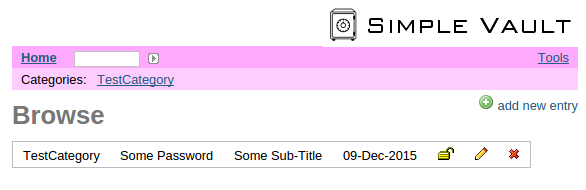
\includegraphics[width=0.95\textwidth]{figures/analysis/simplevault_main.png}
				\caption{Frontpage of SimpleVault.}
				\label{fig:simplevault_main}
			\end{figure}

			\begin{figure}[htbp]
				\centering
				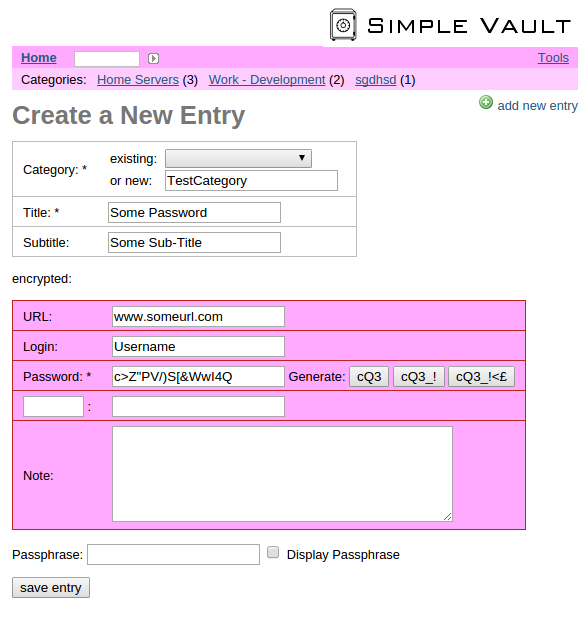
\includegraphics[width=0.95\textwidth]{figures/analysis/simplevault_newpassword.png}
				\caption{Adding a password to be stored in SimpleVault.}
				\label{fig:simplevault_addpassword}
			\end{figure}

			\begin{figure}[htbp]
				\centering
				\begin{subfigure}{\textwidth}
					\centering
					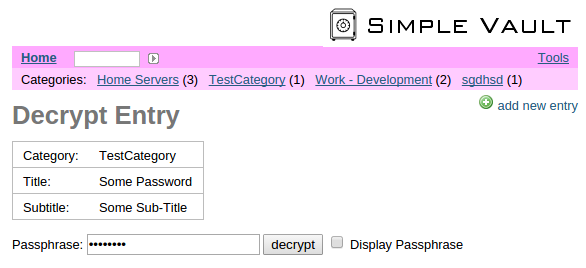
\includegraphics[width=0.95\textwidth]{figures/analysis/simplevault_getpassword.png}
					\caption{Typing passphrase, in order to decrypt stored password.}
					\label{fig:simplevault_getpassword_type}
				\end{subfigure}%
				
				\begin{subfigure}{\textwidth}
					\centering
					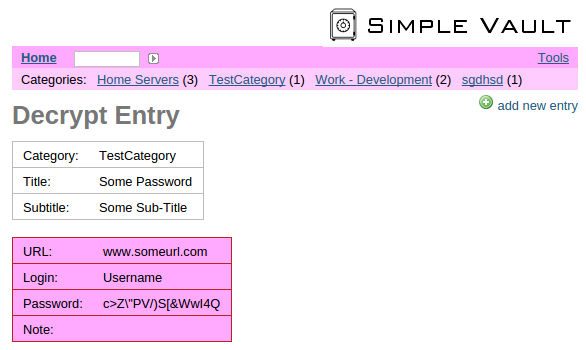
\includegraphics[width=0.95\textwidth]{figures/analysis/simplevault_getpassword_decrypted.png}
					\caption{Decrypted password shown in SimpleVault}
					\label{fig:simplevault_getpassword_decrypted}
				\end{subfigure}
				
				\caption{Process of retrieving a password in SimpleVault.}
				\label{fig:simplevault_getpassword}
			\end{figure}


			Security wise SimpleVault is quite horrible. With what can be taken from the quite poor description of the security of the system, the encrypted data is actally \emph{stored in clear text} on the remote machine, at some point or other. When adding a new entry, the password is sent in \emph{clear text} to the server, which then encrypts it. The developer argues that this is fine, as long as only HTTPS is used, for communicating with the server, but regardless of which protocol is used the password is \emph{still} stored in clear text. Additionally, SimpleVault does \emph{not} use a database system, but stores all contents in a \verb=.txt= file. 

			All in all, SimpleVault is probably a tool \emph{no one} should use. No matter their problem at hand.

		\subsection*{RoboForm}
			RoboForm\cite{roboform} is somewhat a hybrid between the likes of KeePass and LastPass. While at heart, RoboForm is a locally stored password manager, it only exists as a browser extension. Since it only exist as a browser plugin, features such as form auto fill etc. are of course in their repertoire. However, from a ux point of view, the plugin stands out quite a bit from the browser. While this is a relatively small complaint, the usage of design guidelines from both Apple and Google, has helped create platform standards for how apps are supposed look, so the user never feels lost. Additionally, they offer ``RoboForm Everywhere'' cloud synchronisation of the encrypted file. This does however, entail trusting them with safe-keeping the encrypted file.

			Using RoboForm on a single device, renders it as a tool very similar to KeePass, albeit with ``better'' browser integration. Using RoboForm Everywhere results in the same downsides and threats, as previously explained.

		\subsection*{Vaultier}
			At a first glance, Vaultier\cite{vaultier} seems to be everything one would want in the private cloud: Its self-hosted, the latency for actions in the user interface is close to none, and the design of the frontpage is clean. Even installing it comes easy, as it is shipped with a self-contained docker image. However, digging deeper, short comings starts to arise.

			Their choice of organisation is confusing at first. At first you have a workspace, in which vaults are placed. Inside of these vaults, cards are placed. Inside of these cards, passwords are placed. The real problem comes when trying to add items into the vaults. Inside a single vault, you can at most have six cards shown at a time, on a standard 1080p monitor, cf. \ref{fig:vaultier_cards} on page \pageref{fig:vaultier_cards}. The same issue applies when looking at passwords: At most two passwords can be displayed on screen, at a time, cf \ref{fig:vaultier_passwords} on page \pageref{fig:vaultier_passwords}.

			Since RightClick has chosen to have the git repository's history publicly shown, it can be determined the last time it was maintained. That was the 17th of April, 2015\cite{vaultier_history}. It would seem that the project has been abandoned and is dead. As such, it is not a stretch to assume that the project will not be kept up to date, in regards to deprecated dependencies or new-found bugs and security holes.



			\begin{figure}[htbp]
				\centering
				\includegraphics[width=0.95\textwidth]{figures/analysis/vaultier_passwords_lined.png}
				\caption{List of available passwords inside a card, in Vaultier. The dotted line represents the bottom of the browser window, maximized on a 1080p screen.}
				\label{fig:vaultier_passwords}
			\end{figure}
			\begin{figure}[htbp]
				\centering
				\includegraphics[width=0.95\textwidth]{figures/analysis/vaultier_cards_lined.png}
				\caption{List of available cards inside a vault, in Vaultier. The dotted line represents the bottom of the browser window, maximized on a 1080p screen.}
				\label{fig:vaultier_cards}
			\end{figure}

		\subsection{Final Comparisons}
			% Table color shortcuts
			\newcommand{\red}[1]{\cellcolor{red!75}#1}
			\newcommand{\green}[1]{\cellcolor{green!75}#1}
			\newcommand{\grey}[1]{\cellcolor{gray!75}#1}
			\newcommand{\yellow}[1]{\cellcolor{yellow!75}#1}


			While the previous sections covered an in-depth look at the various solutions, it might seem a little overwhelming. Here, the information will be condensed into tables, for a better picture of the differences between the various solutions.

			First and foremost, on table \ref{tbl:web_based} on page \pageref{tbl:web_based}, a clear cut distinction is seen: The solutions that are \emph{able} to be run in the private cloud, and those who isn't. Focussing only on those which actually \emph{can} exist in the private cloud, on table \ref{tbl:passwords} on page \pageref{tbl:passwords} their default approach to passwords are compared. While all of the systems support multiple users in \emph{some} way, they all pretty much share the same sigh on personal passwords: They should not exist. This is primarily a result of nearly all of these being marketed towards teams. For almost all of the solutions, the same approach to solving this shortcoming is the same: Create a new \emph{personal} group for each individual user, in which personal passwords can be stored. Unfortunately, this \emph{must} be considered a workaround, with the exception of PassWork, in which this group is created automatically. 

			Looking at the more technical aspect of the comparison, on table \ref{tbl:agnostic} on page \pageref{tbl:agnostic} a comparison of their agnosticism is made. Most of the solutions are able to be run on multiple platforms, due to being implemented in PHP. Hence, they only require an Apache \emph{(or nginx)} server to be run. Fortunately, both of these have versions for all major operating systems. Unfortunately, there is only one solution that actually has options for various database solutions. \emph{But} the developers note, that this is done at the user's risk, since they're not tested as rigorously.

			By comparing these three tables, it is unfortunately seen that there isn't \emph{one} completely fulfilling the requirements earlier specified.



			\begin{table}
				\begin{minipage}{1.0\textwidth}
					\begin{tabular}{| r | l | l |}
						\hline
						Name 						& Web Based 			& Self-Hostable 		\\
						\hline
						LastPass 					& \green{Yes}			& \red{No} 				\\
						\hline
						KeePass 					& \red{No} 				& \grey{N/A} 			\\
						\hline
						Rattic 						& \green{Yes} 			& \green{Yes}  			\\
						\hline
						Encryptr 					& \red{No} 				& \yellow{Yes} \footnote{Requires editing source files and running own Crypton backend.} 			\\
						\hline
						Passwordstate 				& \green{Yes} 			& \green{Yes}  			\\
						\hline
						Vault \emph{(Zoho)} 		& \green{Yes} 			& \red{No} 				\\
						\hline
						TeamPasswordManager 		& \green{Yes} 			& \green{Yes}  			\\
						\hline
						Simple Safe 				& \green{Yes} 			& \green{Yes}  			\\
						\hline
						Passwork 					& \green{Yes} 			& \green{Yes}  			\\
						\hline
						SimpleVault 				& \green{Yes} 			& \green{Yes}  			\\
						\hline
						RoboForm 					& \red{No} 				& \grey{N/A} 			\\
						\hline
						TeamPass 					& \green{Yes} 			& \green{Yes}  			\\
						\hline
						Vaultier 					& \green{Yes} 			& \green{Yes}  			\\
						\hline
					\end{tabular}
				\end{minipage}
				\caption{Comparison of access method and ownership model, of the available solutions.}
				\label{tbl:web_based}
			\end{table}


			%% Footnotes for Table tbl:agnostic
			\newarray\tblPasswordsFN
			\tblPasswordsFN(1)={Through password grouping.\label{fn:passwords:group}}
			\tblPasswordsFN(2)={Through a commonly used master passphrase, acting as a work-around.\label{fn:passwords:common_masterpassphrase}}
			\tblPasswordsFN(3)={By each user, using their own unique passphrase for encrypting their personal passwords.\label{fn:passwords:unique_masterpassphrase}}
			\begin{table}
				\begin{minipage}{1.0\linewidth}
					\begin{tabular}{ | p{0.30\textwidth} | p{0.25\textwidth} | p{0.15\textwidth} | p{0.15\textwidth} | }
						\hline
						\textbf{Name}  		& \textbf{Supports Multiple Users} 			& \textbf{Personal Passwords} 					& \textbf{Password Sharing} \\
						\hline
						Rattic 				& \green{Yes} 								& \yellow{Yes}\footnote{\tblPasswordsFN(1)}		& \green{Yes} 				\\
						\hline
						Passwordstate 		& \green{Yes} 								& \yellow{Yes}\footref{fn:passwords:group}		& \green{Yes}				\\
						\hline
						TeamPasswordManager & \green{Yes} 								& \yellow{Yes}\footref{fn:passwords:group}		& \green{Yes}				\\
						\hline
						Simple Safe 		& \green{Yes} 								& \yellow{Yes}\footref{fn:passwords:group}		& \green{Yes}				\\
						\hline
						Passwork 			& \green{Yes} 								& \green{Yes}									& \green{Yes}				\\
						\hline
						SimpleVault 		& \yellow{Yes}\footnote{\tblPasswordsFN(3)} & \green{Yes}\footref{fn:passwords:unique_masterpassphrase}		& \yellow{Yes}\footnote{\tblPasswordsFN(2)}\\
						\hline
						TeamPass 			& \green{Yes} 								& \yellow{Yes}\footref{fn:passwords:group}		& \green{Yes}				\\
						\hline 				
						Vaultier 			& \green{Yes} 								& \yellow{Yes}\footref{fn:passwords:group}		& \green{Yes}				\\
						\hline
	   				\end{tabular}
	   			\end{minipage}

				\caption{Comparison of password ownership in self-hostable solutions.}
				\label{tbl:passwords}
			\end{table}



			%% Footnotes for Table tbl:agnostic
			\newarray\tblAgnosticFN
			\tblAgnosticFN(1)={Databases other than MySQL receives less testing.}
			\tblAgnosticFN(2)={No information available to determine.\label{fn:agnostic:no_info}}
			\tblAgnosticFN(3)={Doesn't use a database. Stores passwords in a .txt file.}

			\begin{table}
				\begin{minipage}{1.0\linewidth}
					\begin{tabular}{|r | l | l|}
						\hline
						Name 				& Platform Agnostic 						& Database Agnostic 						\\
						\hline
						Rattic 				& \green{Yes} 								& \yellow{Yes}\footnote{\tblAgnosticFN(1) } \\
						\hline
						Passwordstate 		& \red{No} 									& \red{No} 									\\
						\hline
						TeamPasswordManager & \green{Yes} 								& \red{No} 									\\
						\hline
						Simple Safe 		& \green{Yes}  								& \red{No} 									\\
						\hline
						Passwork 			& \grey{N/A}\footnote{\tblAgnosticFN(2)} 	& \grey{N/A}\footref{fn:agnostic:no_info} 	\\
						\hline
						SimpleVault 		& \green{Yes} 								& \red{No}\footnote{\tblAgnosticFN(3)} 		\\
						\hline
						TeamPass 			& \green{Yes} 								& \red{No} 									\\
						\hline
						Vaultier 			& \green{Yes} 								& \red{No} 									\\
						\hline
					\end{tabular}
				\end{minipage}

				\caption{Comparison agnosticism of self-hostable solutions.}
				\label{tbl:agnostic}
			\end{table}
	
	\section{Academic Research and Tools}
		A number of interesting academic articles and papers was discovered, while researching available solutions from this source. The findings of this, has been condensed into the following list.

		\begin{itemize}
			\item Tapas: Design, Implementation, and Usability Evaluation of a Password Manager \cite{tapas}
			\item Using CardSpace as a Password Manager \& Implementing PassCard - a CardSpace-based Password Manager \cite{cardspace,cardspace_impl}
			\item Stronger Password Authentication Using Browser Extensions
			\item Kamouflage: Loss-Resistant Password
			\item Sesame: A Secure and Convenient Mobile Solution for Passwords
			\item All Your Browser-saved Passwords Could Belong to Us: A Security Analysis and a Cloud-based New Design
			\item Cloud Based Manager Using Privacy-Preserved Biometrics
		\end{itemize}
		

		\subsection*{Tapas: Design, Implementation, and Usability Evaluation of a Password Manager}
			In \cite{tapas}, a new and novel idea is introduced. Rather than using two-factor authentication, a \emph{dual-possession} authentication is used. The basic concept is, that the user has two devices: A smartphone \emph{(wallet)} and a desktop \emph{(manager)}. While it \emph{specifically} states that the manager is a desktop, it is assumed that it might as well be a laptop. The idea is that the manager stores keys for decrypting login information to various sites, while the wallet stores encrypted blobs. The argument is, that even if either device is stolen, offline attacks cannot happen.

			The authentication for storing and retrieving passwords is then based on the fact that the user is in possession of \emph{both} devices, at the time of login. As they describe their solution, it is only possible to access and use passwords on the manager, while the wallet actually stores them. The proposed protocols are:
			\begin{itemize}
				\item Pairing Manager and Wallet
				\item Storing a Password
				\item Retrieving a Password
			\end{itemize}

			Tapas relies on so-called pairing, for easy authentication between wallet and manager, in the remaining protocols. The pairing has to be done in a secret out-of-band channel. During this pairing a private and public key for each device is created, and the public key for the manager is sent to the wallet, and vice versa. This ensures that a secure channel, over a possible hostile connection, can be made in the future.

			While the protocol for storing a password is hardly interesting, the protocol for retrieving a password does present an interesting approach. Retrieval of a password has to be initiated on the \emph{wallet}, or rather smartphone. After authenticating using the previously obtained public keys, they create a secure channel, with perfect forward secrecy, and the wallet sends the encrypted blob to the manager, which then decrypts it and auto-types it in the users browser.

			The team behind Tapas is fairly open regarding what \emph{they} consider the limitations of Tapas. As they see it, there are tree major. First and foremost, the solution relies on an active internet connecting for retrieving passwords. This limitation is unfortunate, but unavoidable with their choice of authentication. It is, however, easily avoided by use of USB tethering or WiFi hotspots, which are standard features in modern smartphones. Secondly, their other limitation is that the smartphone must be charged. Again, a very unavoidable limitation, due to how technology works. The last, and perhaps the only real concern, other than small inconveniences is the fact that Tapas does \emph{not} support multiple devices. It only works with \emph{one} wallet and  \emph{one} manager. Even the wallet cannot access these passwords which is unfortunate, since a lot of the same accounts for a desktop, is also used on a smartphone. All in all, renders it as an unsuited approach to the problem at hand.

		\subsection*{Using CardSpace as a Password Manager \& Implementing PassCard - a CardSpace-based Password Manager}
			In \cite{cardspace,cardspace_impl} the authors design and implement PassCard: A password manager based on CardSpace. CardSpace was Microsoft's client software for their ``Identity Metasystem''. The program was retired as of February 15th 2011, but Microsoft stated that they are working on a replacement \cite{cardspace_cancelled}. This is a service that was discontinued in 2011, and has not been shipped with windows since Windows 8.0. This alone, indicates that this solution is not suitable for any modern devices.

			The basic concept of PassCard, is that the user creates ``Personal Cards''. These cards are able to store various sensitive information, securely. Their solution is a browser extension, which then reads these cards and auto-fills the information. No where in their report, do they describe anything related to adding passwords through PassCard, which leads to believe that his has to be done manually, directly in CardSpace.

			Since CardSpace is a windows only program, this limits the user segment significantly. Additionally, the paper does not mention whether or not they support any kind of multi-device operation, but even if it did it would more than likely be limited to Windows platforms. Hence, the solution is \emph{unusable} for mobile devices, and users of either Mac OS X or Linux. All in all, this solution seems poor in comparison to what we've seen.

		\subsection*{Stronger Password Authentication Using Browser Extensions}
			In \cite{pwdhash} the implementation of PwdHash is discussed. PwdHash's approach, is using a browser plugin as password manager. Their primary issue, seems to be the issue of sending a cleartext password to a remote server for sign up. Their proposal is centered around password derivation, rather than password generation. When typing the password to a site, PwdHash intercepts the password and creates a derived password, using an un-named pseudo random function. The new password is derived from the users original password and the domain name of the site. This derived function is then input into the password field on the website, and the user has retrieved a secure password seamlessly. Salting with the domain name, ensures that even if the user uses the same password for all websites, a unique password is submitted to each site.

			In the paper, the authors make a point of describing each of their steps for avoiding various attacks. Their solution relies on a ``traffic light'', as they call it. When this is green, the user is inputting a password. When it is red, the user is inputting other -- insecure -- information. 

			Additionally, they suggest that the user either inputs a password-prefix, or uses a ``password-key''. Their example of a prefix is \verb=@@=, which the user would have to type every time he or she logged into a site. As an alternative, they suggest using a dedicated keyboard, which they call a ``password-key'', with a button called \verb=password=. In their prototypes they use the \verb=F2= key as a password key.

			To support devices that does not support plugin development, they have a website set up to derive a password, based on a user password and the URL of the website. Additionally they suggest developing a bookmarklet, down the road. As previously discussed, bookmarklets are essentially a security hazard disguised as a usability feature, and should be avoided for all costs.


			After reviewing the paper thoroughly, it is concluded that PwdHash is much more of a secure password derivation tool, rather than an actual password manager. The horrible fact is, that the user still has to input a password for each login. Since users are -- at heart -- lazy, it can be assumed with a fair degree of accuracy, that the majority will re-use the same password over and over. Hence, the only security is that the password is hashed with a \emph{predictable} and very public hash \emph{(the domain name)}. If an attacker was to discover the base password for one site, he or she would then potentially get access to all the users passwords \emph{(assuming the user is lazy)}.

			If, somehow, the user was \emph{not} lazy and had unique passwords for each site, the original problem would still persist. There would be so many unique passwords to remember, that they would be extremely easy to crack using wordlists or simple bruteforce.

			Finally, despite all of their analysis regarding attacks on remote sites, they fail to see that \emph{all} of the same attacks applies to their website for deriving passwords, rendering it a security hazard.

			All in all, PwdHash is not a solution suited for the problem at hand, and actually does nothing for the usability of secure passwords.

		\subsection*{Kamouflage: Loss-Resistant Password}
			In \cite{kamouflage} a whole new paradigm for creating encrypted password databases is suggested: Kamouflage. Kamouflage relies on what they call decoy password sets. One of their primary arguments for implementing Kamouflage is the fact that you can't trust the cloud. Their concern is, that an employee at the cloud service could download the DB and run offline attacks against it. However, they neglect to reason against running this cloud service yourself.

			Imagine a user having a set of passwords, $S$. Then, Kamouflage generates $N$ additional sets, $S_1, \dots S_{N-1}$ to work as decoy password sets. They suggest a default value of $N=1000$. These passwords are generated, using an algorithm based on the work in \cite{cracking}. The aim is generate passwords which are statistically indistinguishable from the \emph{actual} passwords. 

			All of these sets, are then stored side-by-side, in a single file. The idea is then, that the users master password can be run through a cryptographic function and return and index into the file. This index, is then where the \emph{real} password set is stored. A wrong master password would result in another index, which again would result in a decoy password.

			They argue, that with the help of online services, these decoy password sets could be able to be used to detect targeted attacks. However, this both requires that the major websites actually chooses to adopt this technology themselves, and that they need to maintain at least \emph{some} of these passwords on their servers, increasing the needed storage by a decent factor.

			Their scheme for applying encryption to this structure is somewhat convoluted. For each set, they create a password relating to the contents. The algorithm for generating this password, is the same as earlier mentioned. Then, using this password, an encryption key is generated. This key is then used to encrypt the set. After successful encryption of a decoy set, the key is deleted. For the \emph{real} set, the users master password is used to generate an encryption key.

			As the paper states, the layout of the encrypted file, is supposed to make it more difficult for an attacker to access the \emph{correct} password, using offline attacks. Based on this, it appears as if the idea behind Kamouflage is that the encrypted file is stored locally. While their idea of decoy sets might be novel and could potentially be a boost in security, their solution does \emph{nothing} towards solving the problem at hand.

		\subsection*{Sesame: A Secure and Convenient Mobile Solution for Passwords}
			In \cite{sesame} a rather novel idea regarding password managers is described. While the core of Sesame differs in no way from the different solutions described, the process of unlocking the database is where it differs.

			Sesame can be unlocked using voice recognition. Using a remote server, a piece of recorded voice can be used to unlock the password manager. While on a desktop this might be considered unnecessary, it does save the user some hassle of typing in a password on mobile devices.face

			While the idea is novel, and some user might find it exciting and usable, it is fairly limited in regards to platforms. As the authors write themselves, it is intended for smartphones, tablets, smartwatches etc. Hence, the usage for the problem at hand is rather limited.

		\subsection*{All Your Browser-saved Passwords Could Belong to Us: A Security Analysis and a Cloud-based New Design}
			In \cite{browser_saved} they suggest a solution to fix the issues the found, as mentioned in section \ref{subsec:in-browser}. They argue that the data is more secure on a remote machine, run by a company. They prefer to rely on a ``Secure \& Reliable Storage'' service, located in the cloud. They have developed an encryption scheme aimed at protecting the passwords of the users, even though they are stored on a remote machine. 

			However, no matter how secure their scheme is, their suggestion goes against some of the very fundamental requirements mentioned in section \ref{sec:requirements}. As such, their solution is dismissed as not suitable for this specific purpose. 

		\subsection*{Passpet: Convenient Password Management and Phishing Protection}
			In \cite{passpet} a system for managing passwords is suggested: Passpet. It revolves around the idea of petnames. The first time the user uses Passpet, he or she is given a ``persona''. This persona, is essentially a pet, consisting of a random animal logo \emph{(selected from a set of logos)} and a random name. An example of this, is Betty the Fish, as seen on figure \ref{fig:passepet_persona} on page \pageref{fig:passepet_persona}. The randomness is introduced in an attempt to avoid phishing attacks, as the attacker can never know exactly which logo and what name, has been assigned to the user.

			They describe a weird combination of both deriving a password, based on site information and storing data remotely. They derive a password based on a master address \emph{(address of a remote Passpet server)}, a master secret, two constants $k_1$ and $k_2$, and a site label.

			Using passpet only requires the user to press a button, once the correct site label has been entered. This is seen on figure \ref{fig:passpet_main} on page \pageref{fig:passpet_main}.


			\begin{figure}[htbp]
				\centering
				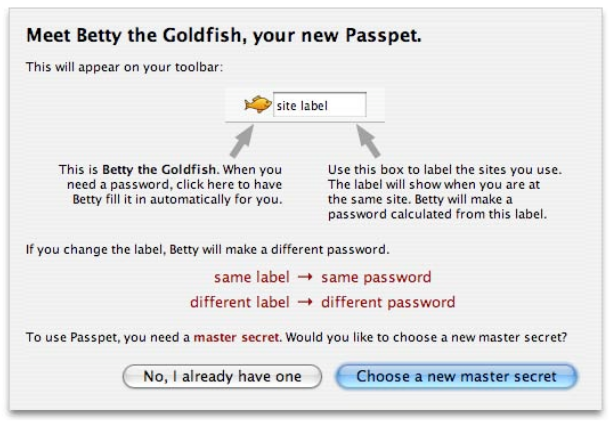
\includegraphics[width=0.95\textwidth]{figures/analysis/passpet_persona.png}
				\caption{Creation of a Passpet persona. \textbf{Source:} \cite[p.4]{passpet}.}
				\label{fig:passepet_persona}
			\end{figure}

			\begin{figure}[htbp]
				\centering
				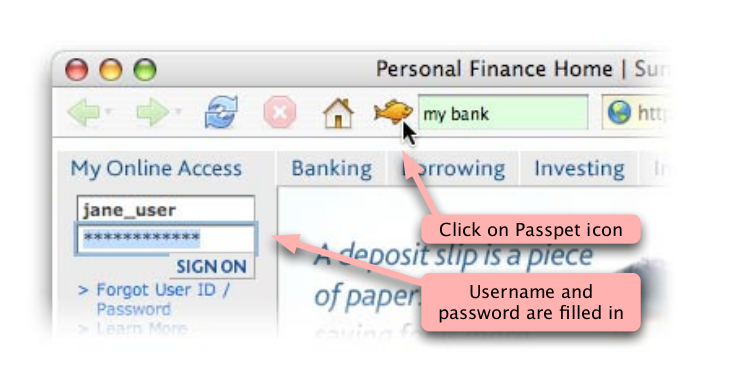
\includegraphics[width=0.95\textwidth]{figures/analysis/passpet.png}
				\caption{Using Passpet. \textbf{Source:} \cite[p.1]{passpet}}
				\label{fig:passpet_main}
			\end{figure}

			Unfortunately, there is an ambiguity in the paper. Several places, a ``Passpet server'' is mentioned, however it is never specifically told who owns this server. 

			To access passwords on other devices, the user will have to input the master address and master secret, and the remote machine will store the constants along with the label list, in order to recreate the passwords. Their description of how a user is authenticated for a second device is poorly described.

			This solution suffers from the same basic issue as described in section \ref{subsec:in-browser}: It only works for website logins, and only in the browser the plugin supports. This, combined with the ambiguity of their report leads to the conclusion that their solution is unfit to solve the problem at hand.


		\subsection*{Cloud Based Manager Using Privacy-Preserved Biometrics}
			Most solutions examined so far, has had the same approach to storing these password databases: Protect them behind a master password. In \cite{busch2014}, however, they argue for another approach: Use biometrics for authenticating access. Building on the prior work of Jain, Nandakumar, and Nagar, they employ Biometric Template Protection, to ensure that the original biometric characteristic can not be reverse engineered. This is then used, to authenticate to the cloud, containing the passwords.


			While this idea \emph{novel}, the usability is limited by our current technology. It is simply a fact, that not all of our devices are equipped with sensors able to detect biometric characteristics. Additionally, there have been voiced some concerns about using biometrics for authentication. All in all, the usage of their solution is not suitable, for the problem at hand.

		\subsection*{A Password Manager that Doesn’t Remember Passwords}
			In \cite{stobert2014} another take a password manager is described. In it, they design and implement a prototype of the software Versipass. Much like the previous section, Veripass has a novel take on authenticating the user, in order to access the password database.

			Existing as a bookmarklet, Veripass presents the user with an image cue, to verify the user. In short, an image cue is a image based password. A image is divided up into squares. A password, is then a selection of these squares. An example of this, is seen on figure \ref{fig:versipass_imagecue} on page \pageref{fig:versipass_imagecue}. The squares are chosen at random, by the system. The use of randomly assigned squares, is done to avoid what they call hotspots in the images, which essentially is areas of a picture which is more likely to be chosen by users, than other areas. 

			\begin{figure}[htbp]
				\centering
				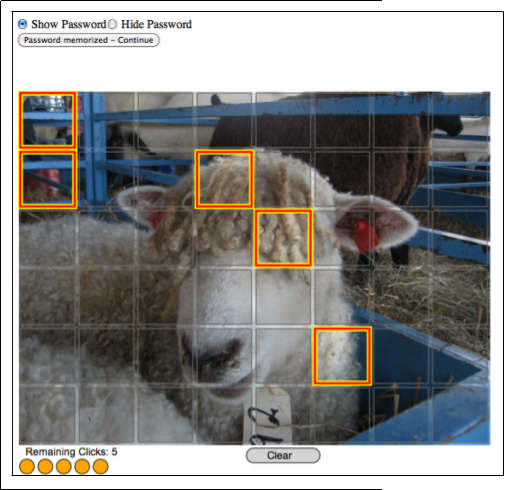
\includegraphics[width=0.95\textwidth]{figures/analysis/versipass_imagecue.png}
				\caption{Versipass' image cue password.}
				\label{fig:versipass_imagecue}
			\end{figure}


		\subsection*{Other Note Worthy Sources}

			In \cite{doodles} they describe using doodles.
\chapter{Designing the System}
	\label{chap:design}
	In the following chapter, the overall design of the system is discussed. First and foremost, the basic architecture is decided, based on the requirements described in section \ref{sec:requirements} on page \pageref{sec:requirements}. Then more detailed subjects are covered, such as how authentication will work, how the solution keeps the users' data safe, and generally how it will work under the hood - so to speak.

	\section{Architecture}
		\label{sec:arch}
		As per the requirements specified in section \ref{sec:requirements} on page \pageref{sec:requirements} the solution will have to be distributed. As such, there are two primary basic paradigms which can be used: Peer-to-Peer and Client-Server. In the following sections the pros and cons of the two will be discussed, and a conclusion of which is more beneficial for the project will be made.

		\begin{figure}[p]
			\centering
			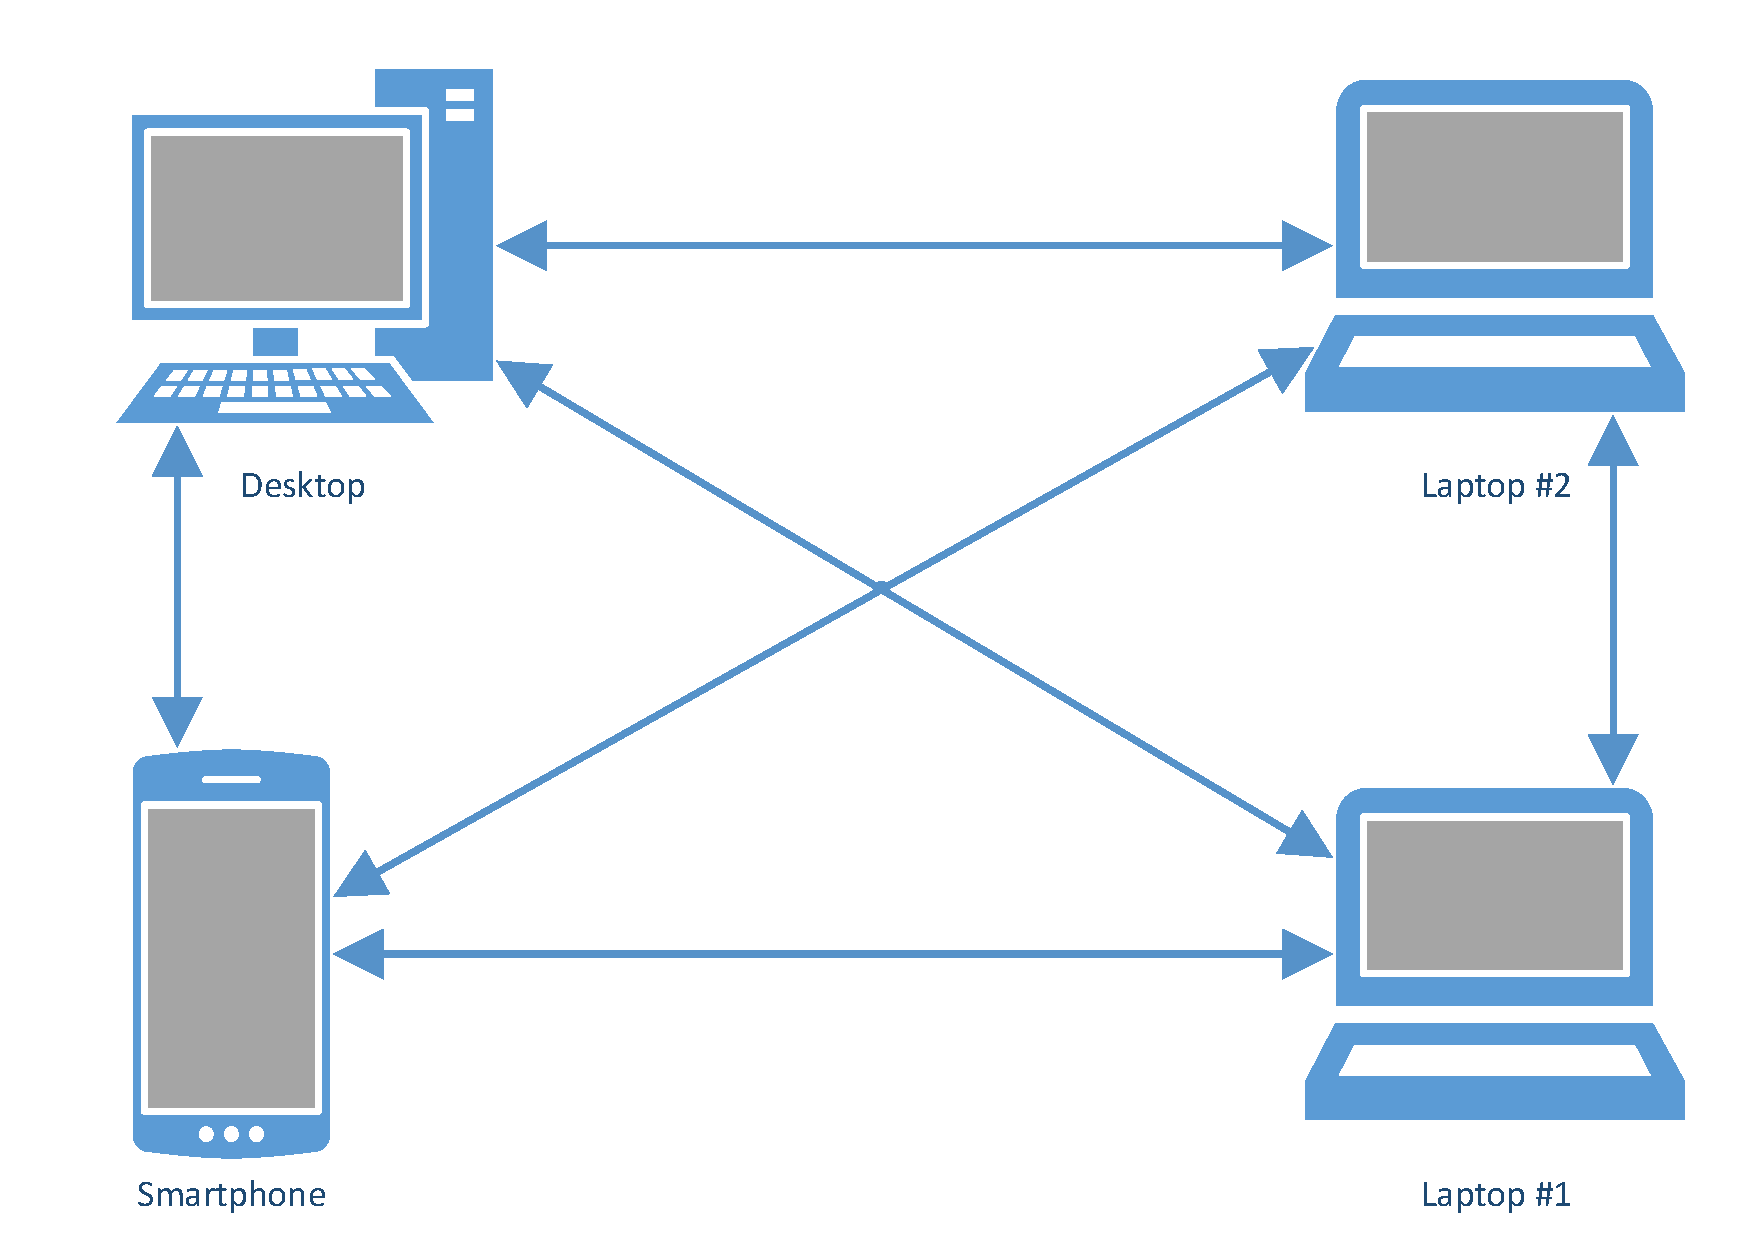
\includegraphics[width=0.8\textwidth]{figures/design/PeerToPeer.pdf}
			\caption{Peer-to-Peer structure visualised.}
			\label{fig:peertopeer}
		\end{figure}

		\begin{figure}[p]
			\centering
			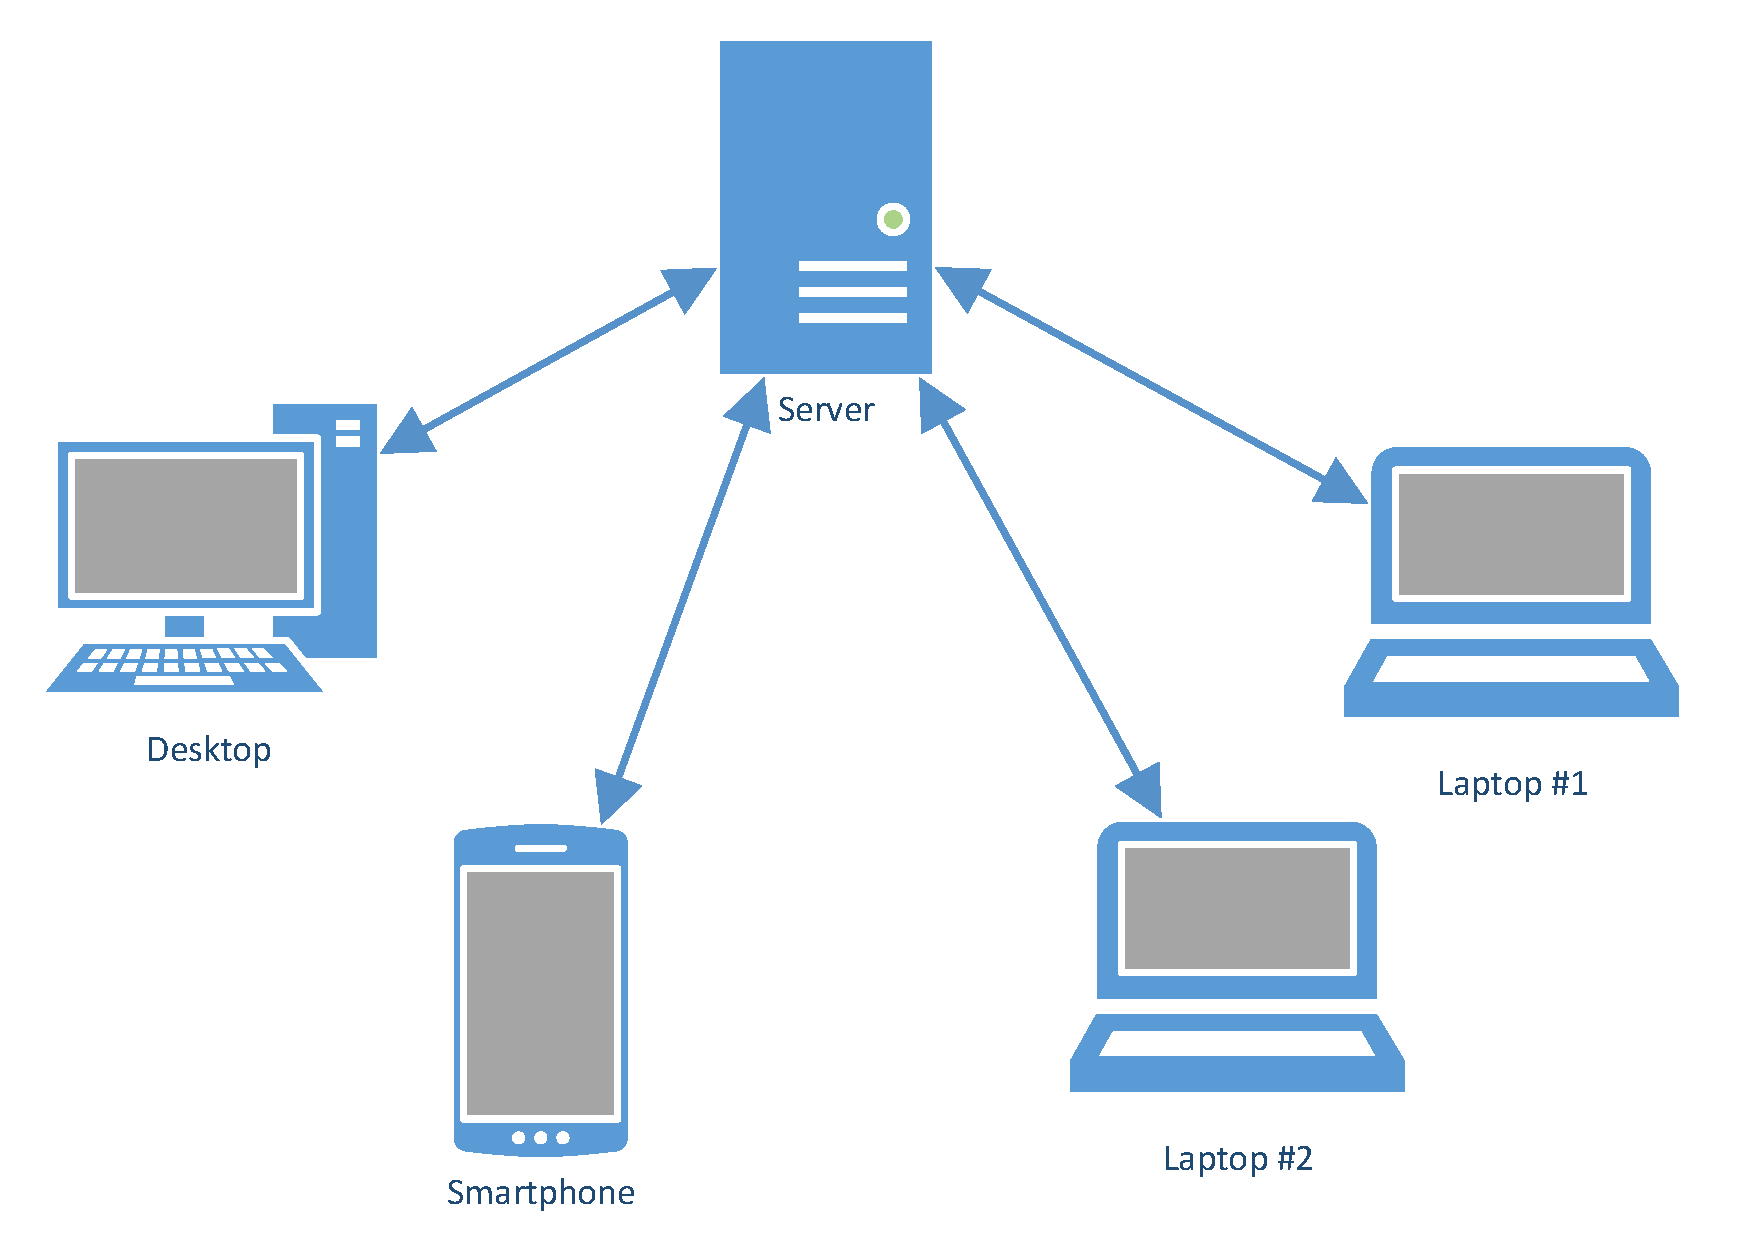
\includegraphics[width=0.8\textwidth]{figures/design/ClientServer.pdf}
			\caption{Client-Server structure visualised.}
			\label{fig:clientserver}
		\end{figure}


		\subsection{Peer-to-Peer}
			Over the past few years, peer-to-peer technology has become ever so more appealing to the masses. Applications such as BittorrentSync applies peer-to-peer technology in an effort to synchronise data between devices. Such an approach could easily be adapted to the problem at hand. A number of a user's devices are online, and synchronises a local password database file between themselves, as visualised on figure \ref{fig:peertopeer} on page \pageref{fig:peertopeer}. This file is then accessed through a native application, on the target device. 

			This approach \emph{definitely} has the lowest overhead of the two: After all it is only devices that needs to have access to the passwords, that need to be setup, maintained, and running for it to be used. However, it does have some drawbacks. Most noticeable, that a native application is required for it to work. This means that for \emph{all} platforms an application needs to be developed. This, in returns, results in a much larger codebase, higher risk of bugs, and a risk of lower consistency across devices. Furthermore, the requirements of logging, as per section \ref{sec:requirements} on page \pageref{sec:requirements}, becomes a lot more difficult, if not to say impossible.

			Additionally, there is a pitfall using this approach. The synchronization requires at least \emph{one} peer with the newest version, to be online for it to work. Let us imagine a user, Paul. Paul has three devices he wish to synchronize passwords to: A desktop, a laptop, and a smartphone -- a very common scenario! Before leaving for a holiday, Paul updates a password on his desktop, while his laptop is closed. Since the smartphone is online at the time, the password is stored there and Paul is perfectly able to access it on his way to the airport. Since it's a long trip, Paul's smartphone runs out of battery along the way. ``No problem!'', Paul thinks and pulls out his laptop -- but oh no! Since the laptop has been offline ever since he left home, it has not received the updated password. And since it is the only online peer -- the desktop at home is turned off and the smartphone has run out of battery -- he can't fetch the newest version. 

			The scenario presented before, can be somewhat mitigated by creating an ``always on peer''. It is a peer in the network, which is always connected and thus always has the newest version available for other peers. However, doing this very much negates one of the strongest arguments \emph{for} this approach: The lower overhead.

		\subsection{Client-Server}
			The client-server paradigm has been the basic model used, since the dawn of the modern internet. When browsing facebook, accessing gmail, or posting a tweet, this is the paradigm employed. It is also the most widespread model used, by the solutions examined in chapter \ref{chap:analysis}.

			Using this approach, there would have to be a dedicated server, acting as the ``master storage'' of passwords. Each client then connects to this server and fetches the passwords. This type of connection is visualised on figure \ref{fig:clientserver} on page \pageref{fig:clientserver}. This does, however, come with its own drawbacks. Since all passwords are stored on a single server, it introduces the risk of a single point of failure. Should the server be compromised or is otherwise unavailable, passwords can not be retrieved \emph{(unless a local cache is used, but this is delving into implementation details)}. It also comes with overhead in form of cost and maintenance. A server will have to be maintained and run 24/7. However, as mentioned in section \ref{sec:privatecloud_cost} on page \pageref{sec:privatecloud_cost}, this can be achieved using low-power devices such as a Raspberry Pi, reducing the financial cost significantly.

			Finally, using the client-server paradigm counters the scenario presented in the previous section. When Paul updates the password from home, the updated password is stored on the server. When he uses his laptop, after his phone has died, it will fetch the updated password from the server.


		\subsection{Conclusion}
			After having weighed the pros and cons of the two approaches, it is decided that a classic client-server architecture will be used. It is deemed that it will create a more seamless experience for the user, and over all will be a more robust solution.

			Another argument why the client-server paradigm is preferable is that if the peer-to-peer paradigm is used, a native application is \emph{required}. This is not the case for the client-server paradigm. A web UI could serve as a front-end, creating a completely identical user experience across devices. But a native application could also be the solution, for the client-server application. Hence, this paradigm allows more freedom of implementation, than peer-to-peer does.

			From here on out, the solution will be split into two parts: The front-end \emph{(client)} and back-end \emph{(server)} -- two very common denominators.

	\section{Communication}
		\label{sec:comms}
		Having determined that the solution will be using the client-server paradigm, the next task is to determine how front-end and the back-end will communicate. There are a number of different available technologies and protocols readily available for use in such a scenario.

		One important fact, that needs to be stated that the back-end is practically equivalent to a web service. As such, 

		\begin{itemize}
			\item Remote Procedure Calls
			\item Remote Method Invocation
			\item Representational State Transfer
			\item SOAP	
			\item Sockets
		\end{itemize}

		\subsection{Remote Procedure Call}
			Remote Procedure Calls, or RPC for short, was introduced by Birrell and Nelson \cite{birell1984} in 1984. The basic concept is to hide the implementation details of invoking a method remotely, for the user.

			The core concept of RPC is that invoking remote methods, are no different than invoking a local method. When the program invokes this method, the underlying software then makes the remote call, hiding these details from the programmer. This is the supposed strength of RPC: It is exactly like invoking a local method.

			An example of an RPC method, could be a method to get a user's data:
			\begin{verbatim}
				getUser(<ID>)
			\end{verbatim}

			For the sake of simplicity various implementations of RPC such as XML-RPC, Corba, and so forth, are considered under the same umbrella.
		
		\subsection{Remote Method Invocation}
			Developed by Sun Microsystems and integrated into the Java API\cite{Downing:1998:JRR:522413}, the Remote Method Invocation \emph{(RMI)} is by many seen as RPC in the object oriented world. While there exists \emph{some} libraries for other languages, Java is the only language to actually natively support RMI. As such, the example will be in Java syntax.

			The basic idea is very much similar to RPC. In RMI an object is transferred to the client, from the server. This can then be invoked from the client, as if it was a local method. On listing \ref{listing:snippet:rmi:server} on page \pageref{listing:snippet:rmi:server} an example server, providing the ``UserService'' is shown. The corrosponding client, is found on listing \ref{listing:snippet:rmi:client} on page \pageref{listing:snippet:rmi:client}. Both examples are missing certian implementation necessary things, like includes and the required interface. The complete files are found in appendix \ref{appendix:rmi}.

			As it is seen, once the stub -- as it is called -- is retrived on the client, there is hardly anything more to it, than when invoking a local method.

			\lstinputlisting[
				frame=single,
				label={listing:snippet:rmi:server},
				caption={UserService Server},
				language=Java,
				breaklines=true,
				gobble=4,
				firstline=8,
				lastline=20]{snippets/rmi/UserServiceImpl.java}

			\lstinputlisting[
				frame=single,
				label={listing:snippet:rmi:client},
				caption={Client using the UserService},
				language=Java,
				breaklines=true,
				gobble=4,
				firstline=3,
				lastline=13]{snippets/rmi/Client.java}

			However, there is a slight drawback: Implementation languages. While RPC implementations such as JSON-RPC makes RPC able to be easily used across multiple languages, this is simply not the case with RMI. Java is -- more or less -- the only language with proper support for this. As such, this solution would be \emph{very} restrictive in regards to actual implementation.

		\subsection{Representational State Transfer}
			\label{sec:design:rest}
			Representational State Transfer, or REST for short, was introduced by Fielding and Taylor \cite{Fielding:2000:PDM:337180.337228} in 2000. REST is an architecture style for designing networked application. It is a stateless, client-server communication \emph{style}, which in most cases uses the Hypertext Transfer Protocol \emph{(HTTP)} protocol and the accompanying HTTP ``verbs''. Traditionally REST uses JSON as body encoding, however it is also possible to use XML.

			The core notion of REST is that resources are bundled in collections, on which the HTTP verbs are used. The API then exposes these collections as Uniform Resource Identifiers \emph{(URIs)} in what is commonly known as endpoints. Using the various HTTP verbs on these endpoints results in actions being invoked on said collections.

			These verbs are for example -- but not limited to-- \verb=GET=, \verb=POST=, \verb=PUT=, \verb=PATCH=, and \verb=DELETE=. These five verbs roughly translates to the basic CRUD operations, as listed on table \ref{tbl:verbs} on page \pageref{tbl:verbs}. So, for instance if one where to \verb=GET= the endpoint of \verb=/api/users= one would get the list of all users on the system. However, most of the time the distinction between \verb=PUT= and \verb=PATCH= is ignored, and \verb=PUT= is allowed to perform partial updates. Table \ref{tbl:rest_example} on page \pageref{tbl:rest_example} shows an example of an API on the \verb=users= resource, showing the result of the respective verbs and their payload. In the example the host of the endpoints have been removed, the prefix could for example be \verb=https://someapi.com/api=, so that an endpoint would be \verb=https://someapi.com/api/users=.

			\begin{table}
				\begin{tabular}{r|l}
					\verb=GET= 		& Read 				\\
					\verb=POST= 	& Create 			\\
					\verb=PUT= 		& Complete update 	\\
					\verb=PATCH= 	& Partial update 	\\
					\verb=DELETE= 	& Delete 			\\
				\end{tabular}

				\caption{How HTTP verbs maps to CRUD operations.}
				\label{tbl:verbs}

			\end{table}

			\begin{table}
				\begin{tabular}{p{0.15\textwidth} | p{0.30\textwidth} | p{0.15\textwidth} | p{0.25\textwidth}}
					Method & Request Body & Endpoint & Ouput \\
					\hline
					\verb=GET= & Empty & /api/users & List of all users \\
					\hline
					\verb=GET= & Empty & /api/users/1 & Details of user with ID of 1 \\
					\hline
					\verb=POST= & \{username:"Daniel", phone:"+45 88888888"\} & /api/users & Creates a new User with the name Daniel and the phone number +45 88888888 \\
					\hline
					\verb=PUT= & \{username:"John"\} & /api/users/1 & Updates the username of the user with ID of 1\\
					\hline
					\verb=DELETE= & Empty & /api/users/1 & Deletes the user with ID of 1\\
				\end{tabular}

				\caption{Example of HTTP verbs used on a REST API for the collection of users.}
				\label{tbl:rest_example}

			\end{table}

		\subsection{Simple Object Access Protocol}
			Simple Object Access Protocol \emph{(SOAP)} was developed by Goshein, Atkinson, Winer, and Box for Microsoft in 1997 \cite{soap_origin}. SOAP is considered an extension of XML-RPC and -- like its predecessor -- uses XML encoding. As implied by its successor SOAP is \emph{strictly speaking} considered an RPC, however due to its uniqueness from ``traditional'' RPCs it is considered separately.

			SOAP can be used with any number of protocols, due to its neutrality, however it is usually used with HTTP or SMPT. Web services relying on SOAP, usually publish a public definition of the available methods, using the Web Service Definition Language \emph{(WSDL)}. This can then be consumed by other clients, making integration with third parties much easier.

			Since SOAP used XML encoding, it is \emph{quite} verbose, and the pure data overhead is significant. Using the same example as from REST, getting the information for a user with ID 1 requires a rather large request body. the XML uses multiple namespaces, the \verb=xmlns= tags are required to define each of them, as \verb=SOAP= and \verb=m= respectively.

			\begin{verbatim}
				<SOAP:Envelope xmlns:SOAP="http://schemas.xmlsoap.org/soap/envelope/">
				    <SOAP:Body>
				        <m:getUser xmlns:m="https://someapi.com/api">
				            <userId>41</userId>
				        </m:getUser>
				    </SOAP:Body>
				</SOAP:Envelope>
			\end{verbatim}

		\subsection{Sockets}
			Underlying all of the previously described technologies are sockets. Sockets are the basic method computers communicate with eachother. Hence, of course it can be used for this purpose. However, there is a \emph{reason} the previous technologies exist: They take care of some of the heavy lifting. Defining a standard for communication, redundancy, standard errors, etc. are but some of the advantages of using either of the previously described technologies. As such, using sockets directly is dismissed without further arguments. 

		\subsection{Making A Choice}
			Making the final choice of how the solution will communicate is important. It sets limitation on future work, and could possibly influence design choices not yet even thought of. 

			First and foremost let us examine RPC. While it \emph{was} the go-to method for achieving the sort of communication which is needed in this project, the issue of implementation remains. Each platform will need its own unique implementation of whichever RPC standard that is chosen. And there is no guarantee that all of these will adhere to the specifications. Additionally, since its usage has become less widespread, it will also hinder further development and integration from third parties, down the line. As such, RPC is dismissed as a possible solution.

			Secondly, there is the RMI. While RMI generally makes remote invocation \emph{very} easy, there is the issue of language restrictions. Since a stub of code is sent from the server to the client, it more or less forces both ends to work using the same language. Additionally, the only proper implementation of RMI is Java's, which even further restricts implementation. As such, RMI is dismissed as a possible solution.

			This leaves SOAP and REST. SOAP is a very ``heavy'' tool, often used in commercial applications, due to its stricter nature. Because of the XML syntax, their payload is \emph{significantly} larger than that of REST using JSON. This results in SOAP being magnitudes slower than REST, cf. \cite{soap_vs_rest}. Additionally there is the matter of support and general adaptation. In the open-source community REST seems to have won the hearts of the crowd. More libraries and tools exists, for aiding in quick development of a RESTful API. This will also make for the optimal base, should other users choose to integrate the solution with their own projects.

			Hence, it is decided that a RESTful approach will be used. 

		\subsection{Comparison With The Requirements}
			\label{requirement:fulfilled:distrib_password}
			\label{requirement:fulfilled:user_storage}

			In the previous two sections, section \ref{sec:comms} and \ref{sec:arch} respectively, a basic architecture and communication model has been chosen. Based on this, it seems only logical to compare our solution at this step, with the requirements previously stated. As such, it is quite clear that since the passwords are stored on a server, which is accessible by all of the user's devices, it is concluded that the solution now fulfil the functional requirement \#\ref{requirement:distrib_password}:

			\vspace{-3ex}\begin{enumerate}
				\setlength\itemsep{0.1em}
				\item Distributed password database
			\end{enumerate}

			Additionally, since the solution will be run on a server \emph{owned} by a user, it can be concluded that the solution fulfil the non-functional requirement \#\ref{requirement:user_storage}:
			\vspace{-3ex}\begin{enumerate}
				\setlength\itemsep{0.1em}
				\item Only use user-controlled storage
			\end{enumerate}

	\section{Securing the Communication}
		Having established the method of communication, it needs to be established that \emph{all} traffic between the client and the server \emph{shall} be encrypted using HTTPS. However, ``use SSL/TLS'' is not the magic solution that it was once thought it was. Over the past few years, more and more attacks have surfaced primarily exploiting attack vectors in what is generally thought to be ``legacy'' options.

		As such, it is almost \emph{required} to heavily limit the available options for SSL/TLS on a service, for it to be considered ``safe''. Table \ref{table:ssl/tls} on page \pageref{table:ssl/tls} contains some of the more recent attacks and what their target is. Previously the recommendation have been to simply use TLS1.0 or higher\cite{ms_tls1.0+}, however this is just no longer viable. 

		As such, a restriction on the choice of implementation platform is made. The chosen library \emph{must} support limiting itself to \emph{only} use TLS 1.2, and likewise it must be able to apply restriction on the cipher suites it supports.

		\begin{table}
			\begin{tabular}{r | l | l}
				\textbf{Attack Name}	& \textbf{Vulnerability In}			& \textbf{Source} 						\\
				POODLE  				& SSL 3.0							& \cite{moller2014poodle}				\\
				``POODLE 2.0'' 			& \emph{Possibly} TLS 1.0 \& 1.1 	& \cite{poodlev2,poodlev2_2}			\\
				DROWN 					& SSL v2  							& \cite{aviramdrown}					\\
				Heartbleed 				& OpenSSL Implementation			& \cite{durumeric2014matter}			\\
				Bar Mitzvah 			& RC4 ciphers and weak keys 		& \cite{mantin2015barmitzvah}			\\
				FREAK 					& ``RSA\_EXPORT'' cipher suites 	& \cite[p.3]{novotnyimplementation}		\\
				WinShock 				& Schell Implementation 			& \cite[p.2]{novotnyimplementation} 	\\
				BEAST 					& TLS 1.0 							& \cite{beast} 								\\
			\end{tabular}
			\caption{Some of the recent SSL/TLS attacks and exploits.}
			\label{table:ssl/tls}
		\end{table}


		\subsection{Comparison With the Requirements}
			\label{requirement:fulfilled:comms}
			\label{requirement:fulfilled:tls1.2}
			While the previous section doesn't add anything new design wise -- strictly speaking -- it applies an implementation \emph{restriction}. As such it is deemed that the solution now fulfil non-functional requirements \#\ref{requirement:comms} and \#\ref{requirement:tls1.2}:
			\vspace{-3ex}\begin{enumerate}
				\setlength\itemsep{0.1em}
				\setcounter{enumi}{5-1}
				\item Use encryption for communication should be viable for at least 5 years
				\item Secure communications, using only TLS 1.2 or newer 
			\end{enumerate}

	\section{Accessing the Back-End}
		Since it has already been determined that the basic architecture of the solution is client-server, it is necessary to determine exactly \emph{which} kind of client there will be needed. 

		There are three obvious types of clients which are not mutually exclusive. First and foremost there is the native client. A native client is \emph{any} client which is developed specifically for a certain platform. An example of a native client could be an Android application or a Windows program. Using tools which are unique to each platform, the client can be integrated tightly with the system. Using for instance the Windows' tray icons or Android's widgets has the advantage of giving the user a more seamless integration with the platform. 

		However, that advantage is -- ironically enough -- also the disadvantage. Since each client is separate from the others, it creates a very departmentalized work flow. While some of the core functionality might be able to be shared across the various clients, it is an undeniable fact that a large portion of the code base will be separated. This introduces higher chances of discrepancy between the various clients. This will in return result in a worse user experience, for any users using clients on multiple platforms. Additionally it is also just more code to review for security flaws.

		The other type of client, and the one growing in popularity in the later years, is the web client. This client is accessed through a browser and is in form of a website. While this does put some restrictions in place, in regards to platform specific technologies, it also ensures that the experience is \emph{identical} across devices. It ensures, that if the user feels at home using the application from a browser on a desktop, he or she will feel at home on a smartphone as well. This also ensures that there is only \emph{one} code base for the client. Finally, this also reduces the chances for implementation errors.

		Finally there is browser plug-ins. While this \emph{definitely} is the most popular type of client for password managers, it also goes in stark contrast with the requirements earlier specified. The issue with \emph{only} using a browser plug-in, is that it in most circumstances this confines the user to storing website passwords, which is \emph{not} desirable.

		All of these three clients are by far mutually exclusive. However, due to constraints of this project it is beneficial to limit the scope to a single interface, with the possibility of further development down the road. For initial prototyping a web UI is the most obvious, since it is the quickest way to achieve cross-platform usage. 

	\section{Storage Encryption}
		In this section various encryption schemes will be compared and discussed. By the end of it, a single solution will be picked. Before getting in too deep with this section, it is needed to re-cap two \emph{very} important requirements:
		\begin{itemize}
			\item Passwords and private information should never be stored or handled un-encrypted anywhere, other than the local device
			\item Password sharing
		\end{itemize}

		The first requirement states that the passwords need to be encrypted when handled in the back-end. Multiple encryption and data schemes could be used for this.

		\subsection{A Single Encrypted Blob}
			One solution, is to simply store \emph{one} large encrypted blob in the back-end. When the user then requests access to a password, this blob is transferred to the front-end, decrypted, and the password can be retrieved. 

			When a new password is generated -- or an old one updated -- the same happens. The front-end fetches the blob, decrypts it, updates or creates an entry, re-encrypts the blob, and then pushes the entire thing to the back-end. The back-end then overrides its own version with the newly received one. This sequence of events is depicted on figure \ref{fig:seq_blob} on page \pageref{fig:seq_blob}.

			\begin{figure}[h!]
				\centering
				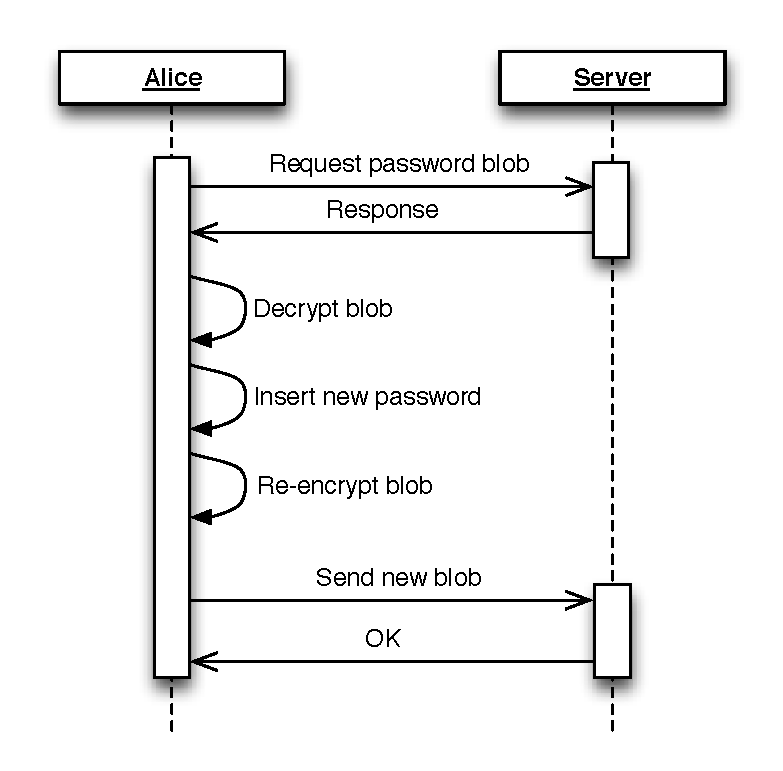
\includegraphics[width=\textwidth]{figures/design/uml/sequence/blob.eps}
				\caption{Squence diagram for creating new password using blob encryption.}
				\label{fig:seq_blob}
			\end{figure}

			The advantage of this, is that the blob practically can be encrypted with whichever scheme the user chooses: The back-end merely sends and receives blobs. However, it also has a \emph{major} drawback. This approach, unfortunately, results in large amounts of overhead: Every time a single entry is accessed, the entire blob needs to be decrypted. Same goes for updating: The entire blob will need to be both decrypted and encrypted again. While this might not be a huge issue with small datasets, it scales horribly for larger sets.

		\subsection{Per Entry Encryption}
			An alternative approach is that encryption could be employed on a per-entry basis. Using this scheme, some of the attributes per entry could then be encrypted. An example of such an entry could be a set consisting of a username, password, and URL. In this specific \emph{example} the password could be the only thing encrypted. 

			Using the same example before, of a password being added or updated, it is clear that encryption-wise, this solution is a lot more lightweight. \emph{Only} the updated / new fields are changed, leaving the remainder of the data unchanged. This sequence of events, is depicted on the sequence diagram on figure \ref{fig:seq_perentry} on page \pageref{fig:seq_perentry}. The drawback to this, is that additional information has the potential of being exposed in the database \emph{(unless the entire entry is encrypted)}.


			\begin{figure}[h!]
				\centering
				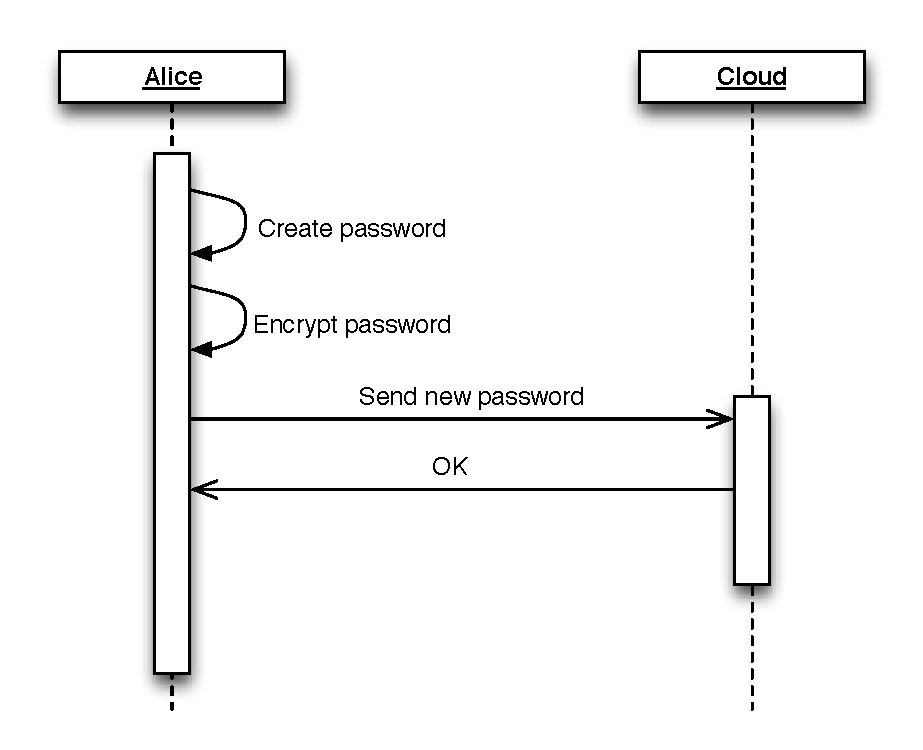
\includegraphics[width=\textwidth]{figures/design/uml/sequence/individual.eps}
				\caption{Squence diagram for creating new password using individual password encryption.}
				\label{fig:seq_perentry}
			\end{figure}

		\subsection{Sharing Is Caring}
			\label{sec:share}
			However, deciding the encryption scheme based on the previous sections is not possible. There is one important aspect, not yet considered: As stated in section \ref{sec:requirements} on page \pageref{sec:requirements} being able to share a password is a requirement. As such, it is important that a user, Alice, is able to share a password with another user, Bob -- and \emph{only} Bob.

			For this feature, an encryption scheme is needed which satisfies the following: Alice can share a single password with Bob, without Bob being able to access the remaining passwords. It should happen purely from Alice's part: No interaction with Bob should be necessary before a password is shared.


			\subsubsection{Proxy Re-Encryption}
				While the exact topic of \emph{password} sharing has not been sufficiently extensively covered in academic literature, topics as secured data sharing has. Since a shared password string is \emph{essentially} data, these techniques and approaches can also apply to this specific case. 

				A fairly new cryptographic concept used for data sharing is proxy re-encryption. A fair amount of academic literature exists on this topic, while \emph{actual} implementations are far more scarce. In ``POSTER: A Certificateless Proxy Re-Encryption Scheme for Cloud-based Data Sharing'' \cite{Wu:2011:PCP:2046707.2093514}, Wi, Xu, and Zhang describe their take on this encryption scheme for data sharing, which they call CL-PRE.

				While a complete analysis of their implementation is far beyond the scope of the current section, a brief overview of how it \emph{fundamentally} works, is seen on fig \ref{fig:sequence:cl-pre} on page \pageref{fig:sequence:cl-pre}.

				In this scenario three parties are involved: Alice, Bob, and a cloud. Both Alice and Bob has their own private/public-key set. Alice wishes to share a password with Bob. The data is encrypted with a symmetric data encryption key \emph{(DEK)}. The encrypted data is then sent to the cloud, alongside an access control list \emph{(ACL)}, a version of the DEK encrypted with Alice's public-key, and a re-encryption key. The re-encryption key is derived from Alice's private-key and Bob's public-key. When Bob requests access to the password, the cloud checks the ACL to see if he has access rights. If he has, the cloud uses a re-encryption algorithm, to transform the DEK into something which can be decrypted by Bob's private-key. Bob then downloads this data, and decrypts it locally using his key.

				%It is quite straight forward how proxy re-encryption could be used for this problem. Each password is encrypted using the DEK. The encrypted DEK is then stored alongside the password. As such, each password has their own unique DEK. When Alice wishes to share a password with Bob, she simply uploads the re-encryption key, derived from her private-key and Bob's public-key, for said password. Bob is then able to access the password. 

				Examining the scalability for this solution, it is shown that it \emph{could} be better. For each password a DEK needs to be stored -- no matter if the password is shared or not. While this is linear scaling, it still creates a fair amount of overhead.

				While this scheme inherently is \emph{everything} that is needed for this particular problem, one slight issue arises. First and foremost it is a recently new technology. This means that implementations are scarce at this point. While this shouldn't matter at this point in time -- since it is the \emph{design} of the solution being discussed -- it \emph{will} have ramifications down the road which needs to be considered. A general rule of thumb is to never ``roll your own'', when it comes to encryption. Existing libraries will have significant more exposure and will possibly have been through one or more security audits. This will most likely mean, that any implementation issues there might have been, should have been discovered and fixed.

				\begin{figure}[h!]
					\centering
					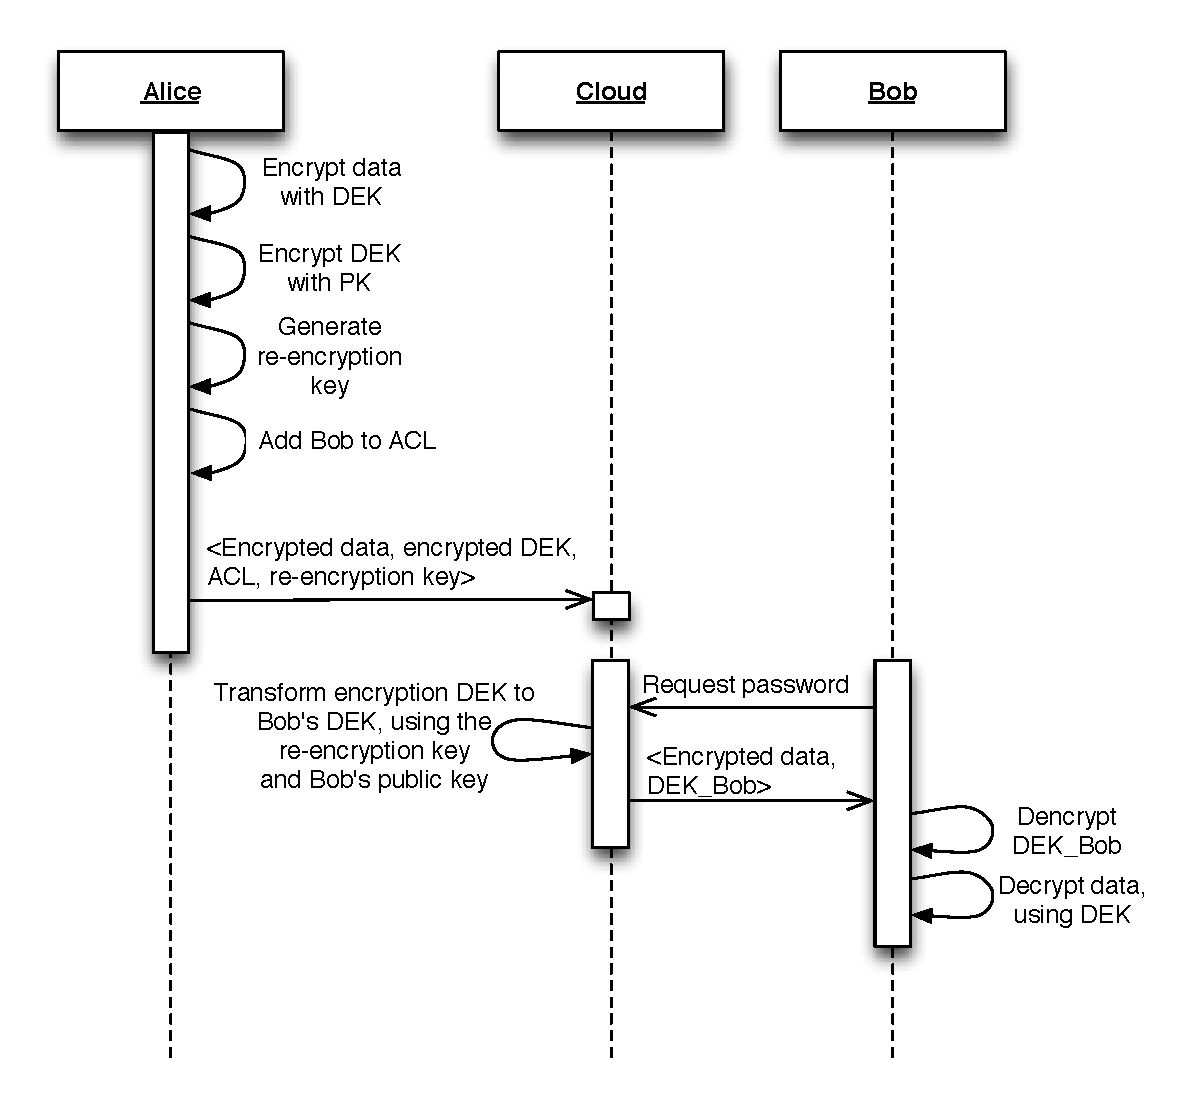
\includegraphics[width=\textwidth]{figures/design/uml/sequence/cl-pre.eps}
					\caption{Sequence diagram for sharing a password, using Wi, Xu, and Zhang's CL-PRE encryption scheme\cite{Wu:2011:PCP:2046707.2093514}.}
					\label{fig:sequence:cl-pre}
				\end{figure}

			\subsubsection{Pretty Good Privacy}
				While the previous section described a start-of-the-art, this approach is more classic. Pretty Good Privacy, or more commonly known simply as PGP, is a scheme dating back to the beginning of the 1990s. 

				PGP uses a combination of symmetric and asymmetric encryption. Whenever a chunk of data needs to be encrypted for sharing, a new symmetric key is generated. The symmetric key is used to encrypt the data. Afterwards, the symmetric key is encrypted using the recipients public-key. Then the encrypted data and the encrypted key is transmitted to the recipient, which can then decrypt the symmetric key, using his own private-key. 

				The reasoning behind this, is that symmetric encryption is \emph{several} magnitudes faster than asymmetric encryption. As such, it is \emph{far} more efficient to encrypt larger documents, using the symmetric key and \emph{then} encrypting said key, than directly encryption the document with an asymmetric key.

				%\textsc{..}
				Using this approach for the problem at hand is quite similar to the previous one. Each password has a unique symmetric encryption key, $SK$, which is never stored directly on the back-end. All users having access to said password, then has a copy of $SK$ encrypted with their own public-key stored. Sharing a password is then as simple as getting the recipients public-key, encrypting the $SK$ with said key, and uploading it to the server. The previous approach is depicted on figure \ref{fig:sequence:pgp} on page \pageref{fig:sequence:pgp}.

				One of the main arguments for using PGP is the fact that symmetric encryption is by far faster than asymmetric. However, in this case the plaintext is relatively small: A password most likely no longer than 72 characters. As such, the performance gained using PGP is pretty much gone. It would hardly take longer to encrypt such a password with asymmetric encryption, than it would for PGP to encrypt a symmetric key.

				Additionally, this solution has the same draw-back as proxy re-encryption. It requires that \emph{all} passwords have an symmetric key stored beside them. The same argument as before can be used again: While it in \emph{no} way can be considered ``bad'' scaling, it could be better.

				\begin{figure}[h!]
					\centering
					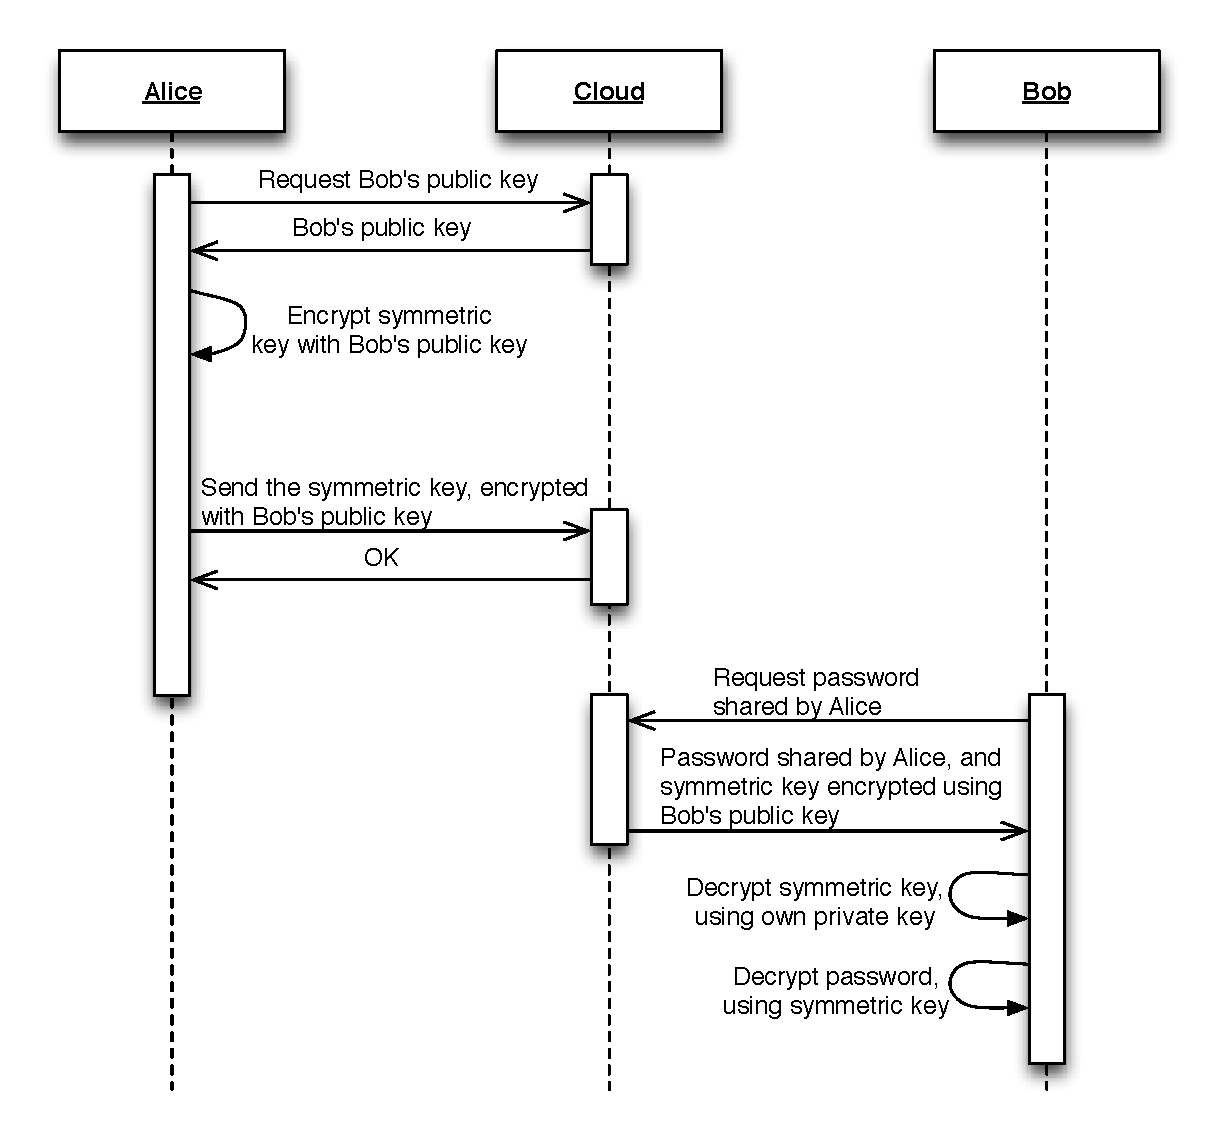
\includegraphics[width=\textwidth]{figures/design/uml/sequence/sharing-pgp.eps}
					\caption{Squence diagram for sharing a password using the PGP scheme.}
					\label{fig:sequence:pgp}
				\end{figure}

			\subsubsection{Asymmetric Encryption}
				\label{sec:assymetric}
				A third option is to directly use asymmetric encryption. Each user has -- like previously -- a private and a public-key pair. Each password is then encrypted using the public-key and stored on the server. To access the password it simply has to be decrypted using the private-key. Sharing the password is simple as well. Simply fetch the public-key of the recipient, encrypt the password using said key, and upload the newly encrypted password. This is shown on figure \ref{fig:sequence:asymmetric} on page \pageref{fig:sequence:asymmetric}.

				One of strongest arguments for the PGP scheme, is that generally asymmetric encryption is significantly faster. However, since the plaintext would be rather small -- most likely below 100 bytes -- this problem is effectively null and void, leaving this scheme a \emph{viable} candidate.

				Using this approach is easily the most simple so far. Alice wishes to share a password with Bob. She fetches his public-key, encrypts the password with said key, and uploads the encrypted password to the back-end. Bob then merely needs to fetch the password and decrypt it, in a process virtually no different from when accessing his own passwords.

				As the astute reader might have figured out, this \emph{strictly} speaking isn't ``sharing'' a password. It is more of a ``sharing by cloning'' procedure. When the original password needs to be updated, it needs to be encrypted once per user it is shared to. This is \emph{definitely} a draw-back, compared to the previous solutions. From a storage perspective, however, this trumps the previous solutions. Storage wise, this is far more efficient than the previous solutions. When a password is shared, it is cloned and stored encrypted with the recipient's public-key, causing only an increased storage \emph{if} a password is shared.

				\begin{figure}[h!]
					\centering
					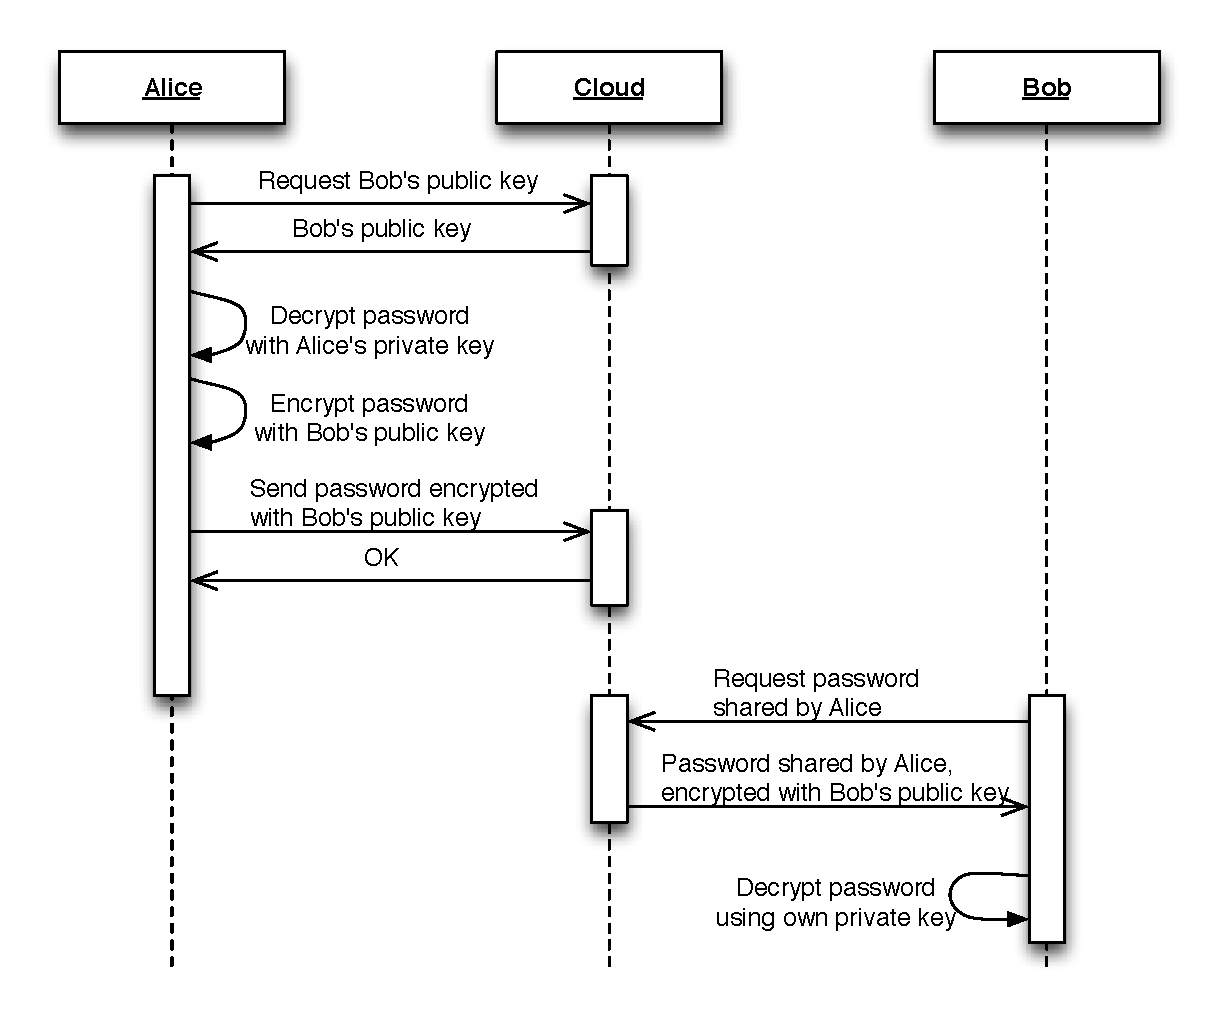
\includegraphics[width=\textwidth]{figures/design/uml/sequence/sharing-asymmetric.eps}
					\caption{Squence diagram for sharing a password, when asymmetric encryption is used.}
					\label{fig:sequence:asymmetric}
				\end{figure}


				%Each user has both a private-key and a public-key stored on the server. When Alice wish to share a password with Bob, she requests the server for Bob's public-key. Once she gets this, she then re-encrypts the password with \emph{Bob's} public-key, and sends this to the server. This way, the password is never handles un-encrypted anywhere other than Alice's front-end. Finally, Bob can easily decrypt the password, using his own private-key. This sequence of events, is shown on figure \ref{fig:seq:assymetric} on page \pageref{fig:seq:assymetric}.

			\subsubsection{Making A Choice}
				\label{sec:encryption_choice}
				Having described three different approaches to solving the problem, it is time to decide exactly which should be used. All of them have their drawbacks -- all of them have their advantages. Since the asymmetric encryption approach has no acronym, it will be referred to as ``Asymmetric'' in the following tables.

				First and foremost, let us examine the availability of tools, cf. table \ref{table:comp:availability}. Admittedly, this should probably carry less weight in the design of the system, however, as mentioned earlier this \emph{will} effect the implementation heavily, should existing libraries not exist. While CL-PRE is just an example of a proxy re-encryption it is a general truth to these algorithms, that at this point in time they are more theoretical than practical -- unfortunately. In stark contrast to this, both PGP and asymmetric encryption algorithms have a plethora of implementations, for just about any combination of hardware and language available. As such, they're the clear favourites in this regard.

				\begin{table}
					\center
					\begin{tabular}{r|l}
						Solution 		& Available Implementations 	\\
						\hline
						CL-PRE 			& \red{Very Rare} 				\\
						PGP 			& \green{Several} 				\\
						Asymmetric 		& \green{Several} 				\\
					\end{tabular}
					\caption{Comparison of availability of implementations of the three encryption schemes.}
					\label{table:comp:availability}
				\end{table}

				Next, it is only fitting to compare the data requirements for these three approaches, cf. \ref{table:comp:data}. As was explained earlier, CL-PRE requires not only an encryption key stored alongside the password, but also a re-encryption key per user said password is shared to. Then there is PGP which only requires an extra encryption key \emph{per} user requiring access. Finally, there is the asymmetric approach which requires no extra data to be stored, due to it only using the users' private and public-keys. As such, the asymmetric approach is \emph{clearly} the favourite in this regard. 

				\begin{table}
					\center
					\begin{tabular}{r|l|l}
						Solution 		& Per Password Value  			& Per Share Value 	\\
						\hline
						CL-PRE 			& \red{Yes} 					& \red{Yes}			\\
						PGP 			& \green{No} 					& \red{Yes} 		\\
						Asymmetric 		& \green{No} 					& \green{No} 		\\
					\end{tabular}
					\caption{Comparison of data usage of the three encryption schemes.}
					\label{table:comp:data}
				\end{table}

				Finally, there is the matter of data processing, which is also an important aspect to take into account, cf. \ref{table:comp:data-process}. Creating a password with CL-PRE involves the following steps: First a symmetric DEK needs to be created, then the password is encrypted with said DEK, and finally the DEK is encrypted using the user's public-key. This totals to $3$ ``cryptographic steps''. PGP is essentially the same. First a new symmetric key is created, then the password is encrypted using that key, and finally the key is encrypted using the user's public-key. Hence, PGP also uses $3$ cryptographic steps. Using asymmetric encryption, however, only a single step is needed: Encrypt the password with the user's public-key.

				For creating a password, the asymmetric approach is clearly the favourite. Not only in the steps involved, but also just from its simplicity. However, this is not \emph{quite} the same when sharing a password. CL-PRE actually only needs a single step for updating a shared a password: Creating the re-encryption key. PGP on the other hand needs two operations: Decrypting the symmetric key, and re-encrypting it with the recipients public-key. Finally, there is the asymmetric approach. This approach needs $n$ operations, per update, where $n$ is the number of people the password is shared to. This \emph{huge} performance loss is due to the fact that it uses sharing by cloning. This is best illustrated with an example: If a password is shared with three people, it means that it exists four times in the back-end: Once encrypted with the owners public-key, and once with each of the people it is shared to. When the password is updated, it needs to be re-encrypted using \emph{each} of these peoples public-keys as well.

				In this case, it is \emph{quite} clear that the asymmetric approach is inferior, when $n$ is large. However, since this overall solution is based around individual password sharing, and not sharing between a group, it is fair to assume that $n$ will be low. As such, the performance loss significantly less than originally assumed.

				All of these three tables are combined into a single large table, on figure \ref{table:comp:complete_schemes} on page \pageref{table:comp:complete_schemes}. Looking at this table, it is quite clear that as long as the assumption of relative few shares per passwords hold, the asymmetric approach is the preferable one to use.

				\begin{table}
					\center
					\begin{tabular}{r|l|l}
						Solution 		& Creating A Password  	& Updating a Password 	\\
						\hline
						CL-PRE 			& \green{$3$} 					& \green{$1$}					\\
						PGP 			& \green{$3$} 					& \green{$2$} 					\\
						Asymmetric 		& \green{$1$}					& \red{$n$} 					\\
					\end{tabular}
					\caption{Comparison of cryptographic steps required for the three encryption schemes. $n$ represents the number of users a given password is shared to.}
					\label{table:comp:data-process}
				\end{table}

				\begin{table}
					\center
					\begin{tabular}{r|l|l|l|l|l}
						Solution 		& \rot{Available Implementations} & \rot{Storage Per Password Value}  	& \rot{Storage Per Share Value}	& \rot{Steps for Creating A Password} 	& \rot{Steps for Updating a Password} 	\\
						\hline
						CL-PRE 			& \red{Very Rare} 	& \red{Yes}		& \red{Yes} 	& \green{$3$} & \green{$1$} \\
						PGP 			& \green{Several} 	& \green{No}	& \red{Yes} 	& \green{$3$} & \green{$2$} \\
						Asymmetric 		& \green{Several} 	& \green{No}	& \green{No} 	& \green{$1$} & \yellow{$n$} \\
					\end{tabular}
					\caption{Complete comparison of the three schemes. $n$ represents the number of users a given password is shared to.}
					\label{table:comp:complete_schemes}
				\end{table}

		\subsection{Asymmetric Encryption Algorithm}
			\label{sec:encryption_choice:rsa_size}
			Having decided on using the asymmetric approach, an algorithm for this needs to be decided. The two contenders for this algorithm is the RSA and ElGamal algorithm. Unfortunately, there does not seem to exist any \emph{sound} papers regarding their comparative strength and efficiency, and as such the choice must be based on something else.

			As such, it is chosen to go with RSA for the reason that its use is simply more widespread. Additionally, a keysize of $4096$ is chosen, as per the recommendations of European Union Agency for Network and Information Security \emph{(ENISA)}\cite[p.37]{enisa}.

			When using RSA, however, it is necessary to be aware of a vulnerability in using ``plain'' RSA. This vulnerability is described in \cite{boneh2000textbook} where an attack reducing the effective security to the half, is described. They also conclude that this can be avoided by using OAEP padding with RSA.

		\subsection{Key Management}
			\label{sec:keys}
			As the astute reader might have realized by now, there is a slight short-coming in what has previously been described. How the private and public-key is stored and transported is omitted \emph{(by choice)}. In an ideal world, all users would automatically have access to the rest of the users' public-keys, and their own private-key would be securely distributed to all devices. However, the world is far from ideal.

			Since the public-key is \emph{not} sensitive information. As such the easiest way to distribute these keys, is simply to store them on the server. This also makes it very easy for the client application to access these keys.

			However, that leaves the private-key. The most secure approach would probably be to let the user manage distributing this key themselves. However, this would end up being a very troublesome process and will lower the over-all user experience. Hence, an encryption scheme for storing the private-key on the server needs to be devised.

			\subsubsection{Choosing an Encryption Algorithm}
				While there exists a plethora of symmetric encryption algorithms, some are more used than others. These are the 3DES, Blowfish, and AES algorithms. As with any of these choices, there exists various pros and cons for each of the algorithms. 

				Several independent papers describe blowfish as the faster algorithm, quoting that since no known vulnerabilities exists for it, it is the best option for symmetric encryption\cite{thakur2011aes,singh2011comparison,verma2011peformance,ramesh2013performance}. While this might very well be true, one can not only compare these algorithms on efficiency, as security is as equally important -- if not more. 

				On the other hand the National Institute of Standards and Technology \emph{(NIST)} -- strictly speaking -- recommends the use of the 3DES and AES algorithms\cite{barker2012sp}, in their report for use of the 3DES algorithm they write:
				\begin{quote}
					\emph{Note: Through the year 2030, Triple DES (TDEA) and the FIPS 197 Advanced Encryption Standard (AES) will coexist as approved algorithms – thus, allowing for a gradual transition to AES. (The AES is another symmetric-based encryption standard approved by NIST.)}\\
					\cite{barker2012sp}
				\end{quote}
				On top of this, ENISA classifies Blowfish as a legacy algorithm, whereas AES is considered future proof\cite[p.20]{enisa}.

				As a consequence it is decided, that the AES algorithm will be used for protecting the private-key, stored on the server. While AES supports a number of different key sizes, AES-256 is chosen for the added security. Additionally, a random IV will need to be generated, due to how AES works.

			\subsubsection{Creating an Encryption Key}
				\label{sec:kdf}
				As with any encryption, AES-256 requires an encryption key. If the key is chosen to be stored on the server, this merely shifts the security risk -- it wont eliminate it. As such, the encryption needs to be based on something which is never stored on the server. The easiest, and by far most logical, way to achieve this, is to use a password. 

				But using a user's password as a asymmetric encryption key will \emph{not} result in enough entropy. Doing this will be \emph{very} insecure. alternatively an encryption key can be \emph{derived} from a password. This is a fairly common task, and is best performed using a so-called Key Derivation Function, or KDF for short. These KDF's are designed to be slow. Where regular hashing algorithms such as SHA-1 are designed to be fast and efficient, KDFs are designed to be exactly the opposite. This is done to slow down a possible brute-force attack against the hash. After all, the regular user will never be the wiser if hashing a single password takes $0.01$ seconds or $1$ seconds. But performing this calculating hundreds of thousands of times will add up, making the computational load for a bruteforce attack \emph{significantly} harder. 

				There exists a \emph{plethora} of various KDFs -- way too many to cover all of them in this section. However, the most widespread KDF is the PBKDF2 algorithm\cite{rfc2898}, which is developed by RSA Laboratories. However, in June 2015 the Password Hashing Competition was concluded\cite{phc}. The competition was held in an attempt to develop a new crypto standard for password hashing algorithms \emph{(practically the same as a KDF)}. Their recommendation is to use the Argon2 algorithm\cite{biryukov2015argon}. Based on this, The Open Web Application Security Project \emph{(OWASP)} made the following recommendation, in regards to password hashing:
				\begin{quote}
					\emph{Select:
						Argon2[*7] when it becomes available. Argon2 is the winner of the password hashing competition and should be considered as your first choice when solid implementations are available.
					}\\\cite{owasp_kdf}
				\end{quote}

				Since Argon2 is such a new algorithm, ``solid'' implementations might very well be difficult to find. But this project will adhere to OWASP's guidelines, as far as possible. As such, it is preferable if the project derives the symmetric encryption key using the Argon2 algorithm. As a final note, avoid multiple users having the same encryption key, a salt will need to be added as well. 

		\subsection{Comparison With Requirements}
			\label{requirement:fulfilled:sharing}
			\label{requirement:fulfilled:passwords_local}
			\label{requirement:fulfilled:encryption}
			Having decided that the solution will revolve around asymmetric encryption, using RSA keys of length 4096 which in return is secured by AES-256 encryption, it can be concluded that the solution fulfils the non-functional requirement \#\ref{requirement:encryption}:

			\vspace{-3ex}\begin{enumerate}
				\setlength\itemsep{0.1em}
				\setcounter{enumi}{4-1}
				\item Use encryption for storage should be viable for at least 5 years
			\end{enumerate}

			Furthermore, due to how the asymetric encryption is handled, not only can the users share passwords, but it can also be enforced, that a password is never even \emph{able} to be decrypted in the back-end. As such, it is concluded that the solution now fulfils the functional requirements \#\ref{requirement:sharing} and \#\ref{requirement:passwords_local}:
			\vspace{-3ex}\begin{enumerate}
				\setlength\itemsep{0.1em}
				\setcounter{enumi}{5-1}
				\item Password sharing
				\setcounter{enumi}{9-1}
				\item Passwords and private information should never be stored or handled unencrypted anywhere, other than the local device
			\end{enumerate}


			%As such, the checklist is updated which is reflected on figure \ref{tab:checklist_encryption} on page \pageref{tab:checklist_encryption}.

				%Having made choices regarding data encryption and protection, in the previous sections, it is now suitable to update the checklist found on figure \ref{tab:checklist_arch-comms} on page \pageref{tab:checklist_arch-comms}. Using the asymmetric approach and protecting the users' keys with a password derived symmetric key, it is clear that the following requirements are now fulfilled

	\section{Authentication}
		\label{sec:design:authentication}
		As with any program handling users' data, there need to be some sort of authentication method in place. Describing the authentication used for this project, will be split up into two categories: First it will be determined exactly how the API will be secured. Once this has been determined, it will be decided how to actually \emph{perform} this authentication.

		\subsection{Securing the API}
			There exists a number of different approaches for securing an API. These range from the built-in protocols in HTTP \emph{(HTTP Basic)} to more advanced enabling users to authenticate using their credentials from Google, for example \emph{(OAuth)}. One important aspect that needs to be stated first, is that this is a \emph{password manager}. Its sole purpose is to enable users to store \emph{strong} passwords to services such as Google. Hence, it would make little to no sense allowing a user to authenticating using their Google account. As such, a very fundamental decision is made here: The authentication scheme \emph{must} work with data stored on the back-end itself.

			\subsubsection{HTTP Basic}
				HTTP Basic is, as the name implies, the most basic form of authentication. It uses standard fields in the HTTP header, containing username and password for authentication purposes. Since it is intended to be a \emph{very} basic authentication method, the password is sent Base64 encoded. Since this is easily decoded, it is considered an extremely insecure protocol if used without HTTPS. Additionally, Basic is vulnerable to replay attacks, if used without HTTPS.

				If, however, combined with HTTPS the insecurity is some-what mitigated, as the password is no longer transmitted in cleartext \emph{(base64)}. However, despite some of the insecurities are mitigated, it still serves the issue that the client will have to store the username and password for usage, as it is needed to be sent with \emph{every} request.

			\subsubsection{HTTP Digest}
				HTTP Digest is another fairly fundamental approach to authenticating with a server, somewhat akin to Basic. Where Basic only Base64 encodes the password, Digest uses a combination of MD5 hashing and and a nonce to avoid replay attacks. 

			\subsubsection{Cookies}
				In the later history of websites, cookies have frequently been used for authentication purposes. Where Basic and Digest requires the credentials to be sent with each request, this approach only requires the so called cookie.

				When the user authenticates to the server, the server issues a cookie. This cookie contains a specific session id, which is also stored on the server. Whenever a request is made to the server, this cookie is then passed along with it. When the server receives said cookie, it checks its internal database and fetches any data relevant to said session. Traditionally cookies are used in combination with stateful websites, which is why it is often not used in RESTful APIs.

			\subsubsection{Tokens}
				Speaking in very general terms, tokens are somewhat similar to cookies: They're a little piece of code, stored in the browser. However, where as cookies are tied to a session on the server, tokens are not. Tokens merely represent a subject, or in this case a user. Upon receiving a request with a token attached, the server then checks the tokens validity and verifies that the subject has access to a given resource. These tokens are also often referred to as ``bearer tokens''.

				Where the previous possibilities pretty much only has a single option for each, tokens are a more diverse option. Generally there exist three primary versions of these tokens:
				\begin{itemize}
					\item Security Assertion Markup Language \emph{(SAML)}
					\item Simple Web Token \emph{(SWT)}
					\item JSON Web Token \emph{(JWT)}
				\end{itemize}
				Since the SAML specification requires the use of SOAP, this is disregarded in this context. The difference between SWT and JWT is that SWT can only be signed symmetrically using the HMAC algorithm, where as JWT \emph{also} supports asymmetric signing using an private/public keypair\cite{auth0_jwt}.

			\subsubsection{Making A Choice}
				While this aspect of the design might seem trivial to some, it is actually a very fundamental and important aspect: It defines how the front-end authenticates with the back-end. While any of the previous approaches are strictly speaking \emph{valid}, some are more obvious than others. The HTTP Digest, for instance, is almost unnecessary compared to the option of just running Basic over HTTPS, and \emph{of course} HTTPS is required.

				That leaves us with Basic, cookies and tokens. Since it has previously been established that it is beneficial for the back-end to be designed in such a way, that third party clients can connect to it, cookies are not optimal. Cookies are primarily intended for the browser and as such, would most likely end up being a hindrance if one should choose to develop a native client.

				As such it is down to Basic or tokens. Basic only has the option of sending the username and password in Base64, as covered earlier. Tokens, on the other hand have the option of sending an entire JSON payload. This opens the possibility for fine tuning the payload down the road and customizing it better to suit the implementation requirements. 

				Trusting the payload of the token requires a certain level of trust. Using symmetrical signing of the JWT for this purpose is \emph{not} suitable. However, using a keypair for signing the JWT \emph{ensures} that the token originated from the server, and not from the client. As such, a certain level of trust can be implied in the token.

				As such, it is chosen that the API will be secured using JWT tokens which will be signed by a private/public keypair.

		\subsection{Obtaining the Token}
			In the previous section it was decided that the API will be protected using JWTs. However, the process of obtaining said tokens were not discussed. There exists a number of different ways to obtain this.

			Anyone working within the industry will without a doubt have at least heard of OAuth and OAuth2. These two authentication protocols are used for users to authenticate to a service, without actually revealing their credentials to said service. Instead they reveal them to Google, for instance, which in return issues a token that is used for authenticating to the service. Earlier arguments were made for why these protocols are \emph{not} suited for this problem, however, certain derived protocols of these exists. Commonly they're known as 2-legged-OAuth and 2-legged-OAuth2. The reason to this is that there is only two actors involved: The user and the service. The OAuth provider, as they're called, are taken out of the equation. While this is definitely a valid option, it is deemed that it is simply too much overhead, for which is essentially a \emph{very} authentication purpose.

			A general consensus amongst professionals using these technologies \emph{(RESTful APIs and JWT tokens)} seem to be, that a simple endpoint expecting a HTTP body with a username and password field, is the way to go, as long as HTTPS is used\cite{jwt.io,auth0_jwt,tkalec}. As such, the same approach will be used for this project.

			Upon receiving the username and password from the user, the back-end compares the password against its database. If it is found to be a match, a new JWT is issued. The process of comparing and validating a user's password is elaborated in section \ref{sec:password}.

			\todo{CHAP and such is not needed, when SSL is enforced 100\%}

		\subsection{Password Storage \& Verification}
			\label{sec:password}
			In the previous section, the process of the server verifying the user's input password was treated as a sort of black box. In this section this process will be examined.

			Today, it is common knowledge that storing passwords in plain text is a \emph{huge} security risk. Salting and hashing passwords, is proper way to implement storage of passwords. However, when choosing a salting algorithm, it is important not to choose algorithms intended for checksums. Algorithms such as SHA-1 and SHA-256 are \emph{designed} to be fast. When trying to mitigate a bruteforce attack on a leaked database, this is \emph{not} desirable.

			As such, it is by far better to use a key stretching algorithm \emph{(or key derivation function)} which is intended to be slow. Since this \emph{exact} topic has already been covered by section \ref{sec:kdf} on page \pageref{sec:kdf}, the same conclusion is made:

			\begin{quote}
				\emph{Select:
					Argon2[*7] when it becomes available. Argon2 is the winner of the password hashing competition and should be considered as your first choice when solid implementations are available.
				}\\\cite{owasp_kdf}
			\end{quote}

		\subsection{Multi-Factor Authentication}
			\label{sec:mfa}
			In the past years there has become more and more focus on security. As a result of this, more and more people are using multi-factor authentication to ensure that access to their personal data is as ``safe'' as possible. 

			In the previous sections only single factor authentication was considered, however, as per the requirements, cf. section \ref{sec:requirements}, the solution will have to support two-factor authentication. All authentication forms fall under one of three categories:
			\begin{enumerate}
				\item Something you know
				\item Something you have
				\item Something you are
			\end{enumerate}
			Using a username and password combination, is falls under the category of ``something you know''. As such, an additional factor needs to be added. 

			In many of the existing systems, this ``extra'' factor of authentication usually falls under the category of ``something you have''. Physical one time passwords, text messages to your phone with a pin, or NemID \emph{(limited to Denmark)} all re-presents a physical entity which the user posses. This means that an attacker not only has to have guessed the user's password, but also have stolen the physical entity. This, in theory, makes it a lot safer.

			However, there are also pitfalls to using possession as an authentication requirement. First and foremost, it is required that the user has the entity available at all times. Without it, he or she can simply not authenticate any more. So in a case of theft, or simple loss, the user is effectively locked out of his or her account. While this definitely is a weakness to the approach, it is deemed that the gain of security highly outweighs the pitfalls.

			\subsubsection{Choosing the Second Factor}
				Using ``something you have'' as a second factor is by far the easiest additional security factor to add to an online system. This involves sending the user a one-time-password \emph{(OTP)}. Some companies do this by providing physical tokens and some by developing their own internal system and accompanying app \emph{(Blizzard Entertainment, for instance)}. While this definitely is an option, it is also by far the most expensive. Dedicated hardware needs to be manufactured, or a separate application needs to be developed. Other companies choose to use text messages as a way of delivering one-time-passwords. The disadvantage to this approach is that a SMS gateway is required.

				A far more universal -- and partially plug'n'play -- approach exists, in the two most common OTP algorithms: HMAC-Based One-Time Password Algorithm\cite{rfc4226}, commonly known as HOTP, and Time-Based One-Time Password Algorithm\cite{rfc6238}, commonly known as TOTP. 

				\textbf{HOTP}\\
				HOTP requires to values to work. First and foremost there is a secret, which is shared behind the HOTP client and the back-end. Secondly, both -- separately -- manages a counter of how many times a OTP has been used. Using these two variables and the HMAC hashing algorithm, the OTP is then calculated. 

				\textbf{TOTP}\\
				TOTP, by many thought to be the successor to HOTP, is roughly the same as HOTP, except it uses a value derived from a timestamp, instead of a counter. The value is derived based on two variables, $X$ and $T0$, where $T0$ is a Unix timestamp from when counting starts, and $X$ is the interval the key is valid for. Usually $T0$ is set to $0$, which is the Unix epoch and $X$ is set to $30$ seconds. The value is then calculated as $T = (now - T0)/X$, cf. \cite[Sec. 4.2]{rfc6238}.

				Both have their respective advantages and disadvantages. The advantage of HOTP is that it is independent from the system clock of the two devices, which is known to drift from time to time. The disadvantage, however, is that the counter needs to be synchronized between the client and the back-end. If the user generates OTPs without using them, they cease to be synchronized. To fix this, they back-end must initiate what the RFC defines as the ``resynch protocol'', which will result in the counter being updated in the back-end. Another drawback is that HOTP requires a counter to be stored in the back-end.

				The advantage of TOTP is that OTPs are generated contentiously. Where the HOTP key lives for a lot longer \emph{(indefinitely)} the TOTP only has a certain window of validity. Common configurations of TOTP lets keys validate for plus/minus two minutes, to account for time drift between the client and the back-end. This, however, is also the weakness of TOTP: Time drift. If the client and the back-end does not operate with the same current time, the OTP will simply not validate.

				Taking the pros and cons into consideration, it is chosen that the TOTP algorithm will be supported in this solution. It is believed that the only inherent draw-back in the algorithm, is mitigated for the most part, by modern systems being fairly good at making sure their internal time is correct.

		\subsection{Comparison With The Requirements}
			\label{requirement:fulfilled:auth}
			\label{requirement:fulfilled:change}
			\label{requirement:fulfilled:two-factor}
			In the previous sections, the various options for securing the API was covered, and it was chosen to use JWT tokens. Additionally, the process of obtaining the token was discussed. Since HTTPS is enforced, a simple API endpoint with the username and password as payload will work quite nicely. It was also decided, that the passwords will be hashed using the Argon2 algorithm, if a decent implementation is available. Otherwise, another key derivation function will be used, in accordance with OWASP's recommendations. As such, it is concluded that the solution fulfil the functional requirements \#\ref{requirement:auth} and \#\ref{requirement:change}:

			\vspace{-3ex}\begin{enumerate}
				\setlength\itemsep{0.1em}
				\setcounter{enumi}{14-1}
				\item Allow user authentication based on a single master password, per user
				\item Allow the user to change his or her master password
			\end{enumerate}

			Additionally, it was decided that the solution will support \emph{optional} TOTP two-factor authentication. As such, it is concluded that the solution also fulfils the functional requirement \#\ref{requirement:two-factor}:
			\vspace{-3ex}\begin{enumerate}
				\setlength\itemsep{0.1em}
				\setcounter{enumi}{16-1}
				\item Support two-factor authentication
			\end{enumerate}

	\section{Attaining Pseudo-Zero-Knowledge}
		As per the requirements it is known that the passwords must never be stored or handled unencrypted on the server. Previously, as an extension of this, it has been argued that letting the back-end as much as having the \emph{ability} of decrypting the stored passwords is ill advised. Hence, there should be no way of inferring the user's password for storing their private-key \emph{(see \ref{sec:encryption_choice} on page \pageref{sec:encryption_choice})} from \emph{anything} stored in the back-end.

		As the reader might have realized by now, \emph{two} passwords are -- unfortunately -- needed. One password for authentication purposes, and one for decrypting the private-key. From now on, these two passwords are known as the authentication password and the decryption password.
 
		The authentication password is the one which is stored on the server, in its salted and hashed form \emph{(see \ref{sec:password} on page \pageref{sec:password})}. This is sent -- in clear text -- to the server for verification purposes. The decryption password is used -- with a salt -- to derive the symmetric encryption key used for the client to decrypt the private-key \emph{(see \ref{sec:keys} on page \pageref{sec:keys})}. At no point in time will the front- or back-end attempt to compare these two passwords, however, it is \emph{strongly} recommended that they be different. As long as they are different it effectively ensures that the back-end can \emph{not} infer the correct decryption key, and as such can never actually inspect the passwords stored on it. This property is dubbed Pseudo-Zero-Knowledge.

		\subsection{Comparison With the Requirements}
			While this feature does not fulfil a requirement directly, it goes to strengthen the way that the requirement regarding un-encrypted data is handled.

	\section{User Hierarchy \& Creation}
		\label{sec:user:diff}
		As with any system, certain functionality should not be exposed to the regular users. As such, user differentiation is needed. There are two different schools of thought when it comes to this: The simple approach and the sophisticated approach.

		The simple approach involved simply storing a boolean value, indicating whether or not the user is an admin or not. While this solution is \emph{very} simple and is most likely the easiest to implement, it has its drawback: There are only two user levels. If one, later down the road, then wanted to add a third user level, this would require large amounts of refactorisation in the code.

		The more sophisticated approach is creating a user hierarchy. This hierarchy would then only consist of two users in the beginning: User and Admin. Based on this hierarchy the solution could enable and disable various aspects based on a user's level. The benefit of this approach, is that later on, several new levels could be added in between the User and the Admin, with varying privileges. How this is stored in the database is up to the implementation, but something as simple as an integer could be sufficient for storing this.

		Since the functionality that needs to be kept away from the regular user, is nothing more than some administrative functionalities here and there, it can be argued that there never will be a need for more user levels. As such, it is chosen to go with the simple approach. 

		Exactly how this user differentiation will be used, will be discussed in the following sections.

		\subsection{Creating Users}	
			Normally, in a solution like the one being designed here, creating the user would be a simple HTTP POST containing the user information. However, since this system will be run by individuals, the owner needs control over exactly \emph{which} users are being created. Hence, open registration is not desirable.

			As such, creating a user will need an ``invite'' of sorts. These invites can then be consumed, in order to create a new user. The most straight forward approach is to let the invite ID simply be the database's auto-incremented ID. However, this might not be a good idea. As most database systems utilize auto-incremented IDs, it would be possibly for an attacker to guess the next ID. As such, the token used needs to be non-sequentially generated.

			The easiest way to do this, is to simply generate a new Universally Unique Identifier \emph{(UUID)} for each invite generated. The UUID is then the token used for accepting an invite. Doing it this way, prevents anyone from guessing the ID of the invite issued next. Putting a lifespan on the invite likewise mitigates a guessing attack, in case of unused invites. For practicalities sake the lifespan will be set to 24 hours.

		\subsection{Creating the First User}
			As was decided in the previous section a user can only be created by an invite issued by an admin. However, when the system is first initalized, the user database would be empty, and there exists no admin who can issue an invite.

			As such, during the initialization process, an admin user will \emph{have} to be created. Using the industry standard, the username and password of this first account will be:
			\begin{verbatim}
				Username:      admin
				Password:      admin
			\end{verbatim}
			Upon first login, the user will then have to be prompted to change not only the password, but also the username, for security purposes.

		\subsection{Breaking the REST Principles On Purpose}
			\label{sec:design:breaking-rest}
			While one of the pillars of REST APIs is that it should be stateless, sometimes this is just not feasible. One example of this, is when enabling two-factor-authentication for users. The back-end \emph{should} verify that the user has gotten the correct secret \emph{(see \ref{sec:mfa} on page \pageref{sec:mfa})}, before actually storing the secret in the database and enabling two-factor authentication. 

			If this verification is not done, the solution will be susceptible to the following scenario, resulting in a user being locked out:
			\begin{enumerate}
				\item User requests to enable 2-Factor-Authentication \emph{(2FA)}
				\item Back-end generates 2FA secret, sends it to user, and stores it
				\item User does not receive correct secret, or forgets to save it, or some other scenario where the secret is not stored correctly
				\item User logs out
				\item User attempts to log in, using the wrong secret
			\end{enumerate}

			As such, a verification step \emph{(which is commonly seen)} is required. This can be easily achieved by having the solution store a cached map, between user ID and the 2FA secret. When a new secret is generated, it is deposited in this cache, instead of the database. A specific API endpoint then exists, for verifying this secret. The verification process is exactly the same process which would be used for logging in. Once the cached secret is verified against the received token, the secret is stored in the database and 2FA is enabled for the user.

			While it is recognized that this violates essential principles of REST, it is deemed \emph{necessary} to do so.


		\subsection{Comparing with the Requirements}
			\label{requirement:fulfilled:multi_user}
			\label{requirement:fulfilled:admin_user}
			\label{requirement:fulfilled:add}
			In the previous sections it has been established how the system will differentiate between admins and users, and now invites will work. As such, it is concluded that the solution fulfil the functional requirements \#\ref{requirement:multi_user}, \#\ref{requirement:admin_user}, and \#\ref{requirement:add}:

			\vspace{-3ex}\begin{enumerate}
				\setlength\itemsep{0.1em}
				\setcounter{enumi}{2-1}
				\item Multi-user support
				\item Support differentiating between admin users and regular users
				\setcounter{enumi}{6-1}
				\item Only admin can add a user -- or invite a user -- to the solution
			\end{enumerate}

	\section{Auditing of Access}
		\label{sec:audit}
		Since it is peoples passwords being handled, some sort of audit log is preferable. Simply put, an audit log contains entries of when certain actions took place. For instance, it could be whenever a user authenticates the service, an audit log entry -- or simply entry -- is generated. Later on, the user can review these entries. This way, the user can easily see if an authentication has taken place, somewhere that he or she was not.

		When creating an audit log, it is very tempting to simply create an entry for \emph{everything}. However, while this will contain the data the user would need, it will be \emph{too} much data. Not only for the user to review, but also for the back-end to store. As such, first and foremost, it is necessary to determine exactly which events are necessary to log.

		Obviously, there is the matter of authentication. Both successful and failed authentication attempts will have to be logged. With this information, a user can quickly determine if access has been made from a device which he or she has not used. Furthermore, access to passwords should be logged. This access can call into any of four categories of actions: Create, read, update, and delete. These actions also apply to shared passwords. While the create actions could be used to denote a newly shared password, for the sake of usability a Share action is used instead. The remaining actions, read, update, and delete, also applies to shared passwords. As such, it is concluded that there will be \emph{seven} actions:
		\begin{enumerate}
			\item Success
			\item Failure
			\item Share
			\item Create
			\item Read
			\item Update
			\item Delete
		\end{enumerate}

		\begin{table}
			\begin{tabular}{r | c | c | c }
							& \textbf{Authentication} 		& \textbf{Passwords} 		& \textbf{Shared Passwords} 	\\
				\hline
				Success 	& \cmark 						& \xmark 					& \xmark 						\\
				Failure 	& \cmark 						& \xmark 					& \xmark 						\\
				Share 		& \xmark 						& \xmark 					& \cmark 						\\
				Create 		& \xmark 						& \cmark 					& \xmark 						\\
				Read 		& \xmark 						& \cmark 					& \cmark 						\\
				Update 		& \xmark 						& \cmark 					& \cmark 						\\
				Delete 		& \xmark 						& \cmark 					& \cmark 						\\
			\end{tabular}
			\caption{Which targets the various actions describe}
			\label{table:actions}
		\end{table}

		Each of these actions apply to either authentication \emph{(1 \& 2)} or passwords \emph{(3-7)} and shared passwords \emph{(2 \& 4-7)}. This relation is also shown on figure \ref{table:actions} on page \pageref{table:actions}.
		
		However, this information is hardly enough, to properly audit the entries. As such, information such as the timestamp for the event and the hostname of the machine, will greatly aid in the process of auditing. 

		\subsection{Comparison With Requirements}
			\label{requirement:fulfilled:audit}
			Having decided on what data should be logged for audit, it is concluded that the solution now fulfil the functional requirement \#\ref{requirement:audit}:
			\vspace{-3ex}\begin{enumerate}
				\setlength\itemsep{0.1em}
				\setcounter{enumi}{13-1}
				\item Extensive auditing
			\end{enumerate}

	\section{Modelling the System}
		\label{sec:modelling}
		In the previous sections, all of the various requirements have been thoroughly discussed. In this section, all of these requirements will be condensed into the actual models used, in the system. 

		\subsection{The User Model}
			The User model is the most basic structure in the project. It represents -- obviously -- each individual user. As such, three very basic attributes need to be present: Username, password, and salt. The username will appear in cleartext, and the password and salt are the results of the hashing algorithm and is most likely in hexadecimal format. While some hashing functions store the generated salt in the resulting password hash, some do not. As such it has been deemed beneficial to have an dedicated variable for this. Next, in section \ref{sec:user:diff} on page \pageref{sec:user:diff} it was determined that user and admin differentiation would be done using a simple boolean and for this purpose a field called isAdmin is added.

			In sections \ref{sec:encryption_choice} and \ref{sec:kdf} on pages \pageref{sec:encryption_choice} and \pageref{sec:kdf}, respectively, it was determined that asymmetric encryption will be used. As such, a private-key and a public-key will need to be stored, additionally it was determined that a salt and IV needs to be stored. 

			Finally, as per section \ref{sec:mfa} on page \pageref{sec:mfa}, there a 2FA secret will need to be stored. Furthermore, a boolean toggle value determining whether or not 2FA is enabled for said user, is stored as well.

			As such, the final User model contains the fields listed on table \ref{fig:model:user} on page \pageref{fig:model:user}.

			\begin{table}[p]
				\centering
				\begin{tabular}{r|l}
					\textbf{Attribute} 		& \textbf{Type} 		\\
					ID 						& Unknown 	\\
					username 				& String 	\\
					password 				& String 	\\
					salt 					& String 	\\
					isAdmin 				& Boolean 	\\
					privateKey  			& String 	\\
					publicKey 				& String 	\\
					IV 						& String 	\\
					privateKeySalt 			& String 	\\
				\end{tabular}
				\caption{Fields of the User model}
				\label{fig:model:user}
			\end{table}

		\subsection{The Category Model}
			\label{sec:model:category}
			Before delving into the core model, the Password model \emph{(see the following section)} it is required to cover an auxiliary model: The Category. Since it has already been determined that it is required for the solution to structure passwords in multiple levels, a data structure for this is required.

			First and foremost, it is important to realise that the classical ``folder'' structure, is nothing more than what is commonly known as a tree. Trees consists of internal nodes and leafs. Nodes have children. These children can be other nodes, or a leaf. A leaf is a final child -- it is last element in the branch. An example of such a tree is seen on figure \ref{fig:example:tree} on page \pageref{fig:example:tree}.

			This structure can be translated very easily to the structure needed for password organization. The root and the internal nodes represent the various categories, and the leafs represent the passwords. As such, it will look like figure \ref{fig:example:passwordtree} on page \pageref{fig:example:passwordtree}.

			Multiple data structures exist to solve this exact problem. The simplest of them all, is the adjacency list. In this approach, each element simply stores a reference to either its parent or its children \emph{(top-down or bottom-up)}, depending on the implementation. This allows for the structure to be stored ``flat'', i.e. in a table, or an array, and when required the actual tree can be built from the data. Examples of these notations are found on tables \ref{table:example:tree:buttomup} and \ref{table:example:tree:topdown} on pages \pageref{table:example:tree:buttomup} and \pageref{table:example:tree:topdown}, respectively. The examples are based on the tree structure from figure \ref{fig:example:passwordtree} on page \pageref{fig:example:passwordtree}.

			While this approach might inherently be slower than other algorithms, cf. \cite{heirarchial_database}, it is believed that due to the relatively small datasets -- which is \emph{assumed} to be used -- it will have little effect. As such, the simplicity of the storage scheme a makes it perfect for this use.

			\begin{table}[p]
				\centering
				\begin{tabular}{c|c|c}
					\textbf{ID} 	& 	\textbf{Name} 	& \textbf{Parent} 	\\
					\hline
					\hline
					1 				& Root 				& Null 				\\
					2 				& Category1 		& 1 				\\
					3 				& Category2 		& 1 				\\
					4 				& Category1.1 		& 2 				\\
					5 				& Category1.2 		& 2 				\\
				\end{tabular}
				\caption{Flat tree structure, using bottom-up adjacency}
				\label{table:example:tree:buttomup}
			\end{table}
			\begin{table}[p]
				\centering
				\begin{tabular}{c|c|c}
					\textbf{ID} 	& 	\textbf{Name} 	& \textbf{Children} \\
					\hline
					\hline
					1 				& Root 				& [1,2] 			\\
					2 				& Category1 		& [4,5] 			\\
					3 				& Category2 		& [] 				\\
					4 				& Category1.1 		& [] 				\\
					5 				& Category1.2 		& [] 				\\
				\end{tabular}
				\caption{Flat tree structure, using bottom-up adjacency}
				\label{table:example:tree:topdown}
			\end{table}

			\begin{figure}[h!]
				\centering
				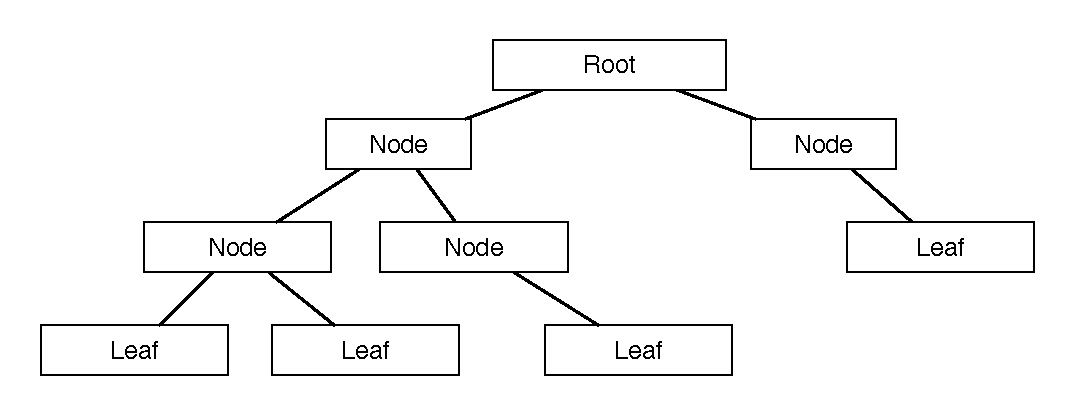
\includegraphics[width=\textwidth]{figures/design/general/generic-tree.eps}
				\caption{Example of a tree.}
				\label{fig:example:tree}
			\end{figure}
		
			\begin{figure}[p]
				\centering
				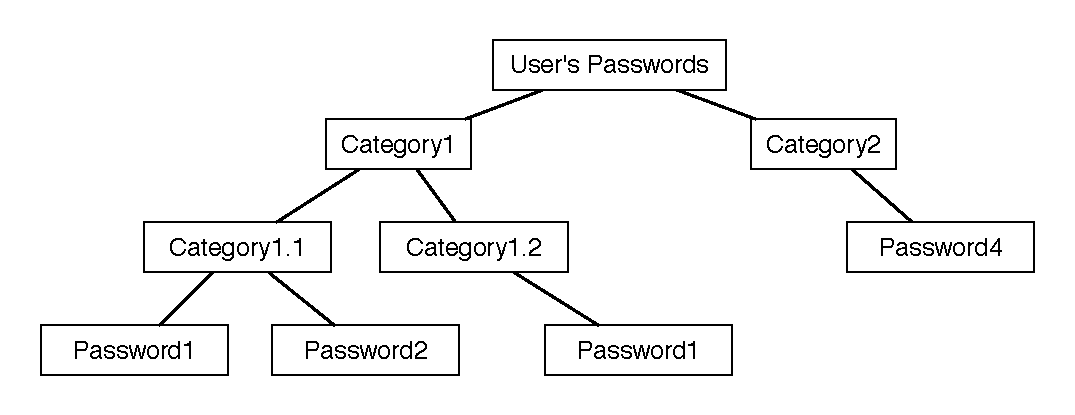
\includegraphics[width=\textwidth]{figures/design/general/password-tree.eps}
				\caption{Example password structure in a tree.}
				\label{fig:example:passwordtree}
			\end{figure}

			As such, it is determined that the Category model will contain the fields listed on table \ref{fig:model:category} on page \pageref{fig:model:category}. On figure \ref{fig:relationship:category-user} on page \pageref{fig:relationship:category-user}, the relationship between the Category model and the User model is depicted, as well as the recursive definition of structure with itself.


			\begin{table}[p]
				\centering
				\begin{tabular}{c|c}
					\textbf{Attribute} 		& \textbf{Type} 		\\
					ID 						& Unknown 	\\
					title 					& String 	\\
					owner 					& User ID 	\\
					Parent / Children List 	& Parent ID / List of Children IDs 	\\
				\end{tabular}
				\caption{Fields of the Category model}
				\label{fig:model:category}
			\end{table}
			\begin{figure}[p]
				\centering
				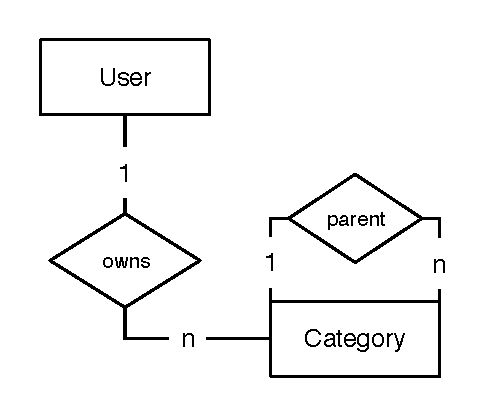
\includegraphics[scale=0.75]{figures/design/uml/erd/user-category.eps}
				\caption{The Category models relationship with the User model.}
				\label{fig:relationship:category-user}
			\end{figure}

			%\subsubsection{Algorithm: Generating the Structure}

			%\subsubsection{Algorithm: Deleting a Category}

		\subsection{The Password Model}
			\label{sec:model:password}
			Having described the Category model fully, the Password model can now correctly be explained. First and foremost it will consist of the fields that generally make up a password entry: A title, a username, a password, an URL, and a note. However, the passwords needs a way to connect with a user. For this purpose, a reference to the User models ID is needed. This reference is known as owner, i.e. the user who owns the password. Finally, to achieve the structure, as described in the previous section, a password is a child of a category. Hence, the Password model will need a reference to a parent Category's ID. These references are also depicted on figure \ref{fig:relationship:password} on page \pageref{fig:relationship:password}.

			As such, the final Password model contains the fields listed on table \ref{fig:model:password} on page \pageref{fig:model:password}.

			\begin{table}[p]
				\centering
				\begin{tabular}{c|c}
					\textbf{Attribute} 		& \textbf{Type} 	\\
					ID 						& Unknown 			\\
					title 					& String 			\\
					username 				& String 			\\
					password 				& String 			\\
					url						& Boolean 			\\
					note  					& String 			\\
					owner 					& User ID 			\\
					parent 					& Category ID 		\\
				\end{tabular}
				\caption{Fields of the Password model}
				\label{fig:model:password}
			\end{table}
			
			\begin{figure}[p]
				\centering
				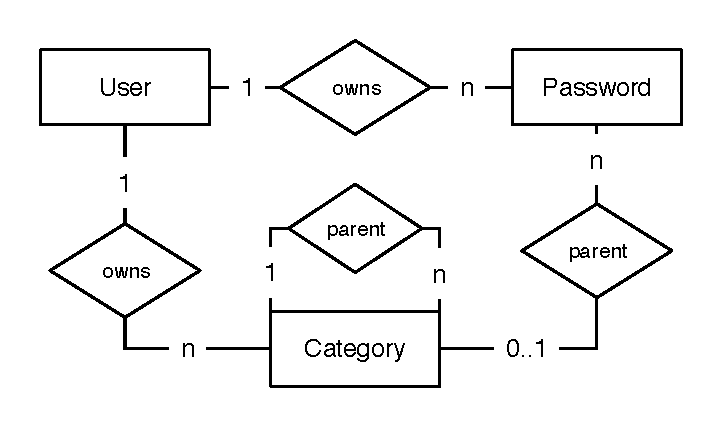
\includegraphics[scale=0.75]{figures/design/uml/erd/user-password-category.eps}
				\caption{A Password's connections to the User and Category models.}
				\label{fig:relationship:password}
			\end{figure}

			\subsubsection{One Hundred Thousand Entries}
				\label{sec:model:password:size}
				As the requirements state, the solution will have to store at least 100.000 entries. Based on the attributes defined on table \ref{fig:model:password}, the feasibility of this is investigated. 

				It is assumed that an ID is stored as an integer, and is four bytes in size. Additionally, the traditional length of text fields are used \emph{(255 characters)} which is stored as 256 bytes. Finally, there is the matter of the password. From sections \ref{sec:encryption_choice} and \ref{sec:encryption_choice:rsa_size} on pages \pageref{sec:encryption_choice} and \pageref{sec:encryption_choice:rsa_size}, respectively, it is known that this is encrypted using a 4096 bit RSA key. As it is known, the output of the RSA algorithm is always the same length as the key. Hence, the output is 4096 bits -- or 512 bytes -- long. Finally, since the output is binary, it needs to be base64 encoded, for proper transmission and storage. Due to the inner workings of the base64 encoding, the size of the encoded text is $4\lceil*{n/3}$ of the original text, where $n$ is the number of bytes of the input. As such, the base64 encoded version of the encrypted password, has a size of $684$ bytes. Using the values found on table \ref{tab:model:password:size}, it is concluded that the total size for each entry is $1465$ bytes.

				Using the requirements minimum number of entries \emph{($100.000$)}, this results in a total size of $146.5$ megabytes, for the passwords alone. While this might sound as much, in today's world where flash storage reaches $64$ gigabyte at an affordable price, and mechanical storage is measured in terabytes, this is hardly causes an issue.

				\begin{table}
					\centering
					\begin{tabular}{l | r | r}
						\textbf{Name}  			& \textbf{Type} 		& \textbf{Size \emph{(in bytes)}} 		\\
						\hline
						ID 						& Integer 			& 4						\\
						title 					& String 			& 256					\\
						username 				& String 			& 256					\\
						password 				& String 			& 684					\\
						url						& Boolean 			& 1						\\
						note  					& String 			& 256					\\
						owner 					& User ID 			& 4						\\
						parent 					& Category ID 		& 4						\\
						\hline\hline
						\textbf{Total} 			& - 				& 1465
					\end{tabular}
					\caption{Variable size of the attributes for the Password model.}
					\label{tab:model:password:size}
				\end{table}


		\subsection{The Shared Password Model}
			Having decided that the password sharing mechanism will be sharing by cloning, 

			Sharing a password can be achieved easily, by simply storing a reference to a user's password, under the ownership of another user. As such, each shared password entry will contain a reference to the original password. Using this reference, fields such as the username etc., can easily be obtained. However, since the \emph{actual} password is encrypted using each users individual key, this needs to be stored as well. To let the user receiving the shared password organize it as he or she sees fit, a reference to a Category ID is needed. Finally, references to the original owner and password, will make certain operations a lot easier. These relations are all shown on figure \ref{fig:relationship:sharedpassword} on page \pageref{fig:relationship:sharedpassword}, albeit the internal relations between User, Password, and Category has been omitted for clarity.

			As such, it is determined that the Shared Password model will contain the fields listed on table \ref{fig:model:sharedpassword} on page \pageref{fig:model:sharedpassword}. 

			\begin{table}[p]
				\centering
				\begin{tabular}{c|c}
					\textbf{Attribute} 		& \textbf{Type} 		\\
					ID 						& Unknown 		\\
					owner 					& User ID \\
					originOwner 			& User ID \\
					parent 					& Category ID \\
					password 				& String \emph{(Base64 Encoded)} \\
					originPassword 			& Password ID 		\\
				\end{tabular}
				\caption{Fields of the Password model}
				\label{fig:model:sharedpassword}
			\end{table}

			An example such an entry could be the following. Two users exists, as seen on table \ref{fig:example:sharedpassword:users} on page \pageref{fig:example:sharedpassword:users}, Alice and Bob \emph{(irrelevant user data has on purpose been left out)}. Alice owns a password with the title ``SamplePassword'', the details of which are shown on table \ref{fig:example:sharedpassword:samplepassword} on page \pageref{fig:example:sharedpassword:samplepassword}. Alice now wishes to share this password with Bob. As such, an entry is created, containing the information found on figure \ref{fig:example:sharedpassword:sampleshare} on page \pageref{fig:example:sharedpassword:sampleshare}.
			\begin{table}[p]
				\centering
				\begin{tabular}{r|l}
					\textbf{ID} 		& \textbf{Username} \\
					42 					& Alice 			\\
					1337  				& Bob 				\\
				\end{tabular}
				\caption{Sample user data}
				\label{fig:example:sharedpassword:users}
			\end{table}

			\begin{table}[p]
				\centering
				\begin{tabular}{c|c}
					\textbf{Attribute} 		& \textbf{Type} 											\\
					ID 						& 127 														\\
					title 					& SamplePassword 											\\
					username 				& SampleUser 												\\
					password 				& QmFzZTY0IEVuY29kZWQgUGFzc3dvcmQ= 							\\
					url						& www.some.com 												\\
					note  					& This is a sample password 								\\
					owner 					& User ID 													\\
					parent 					& Category ID 												\\
				\end{tabular}
				\caption{Sample password owned by Alice}
				\label{fig:example:sharedpassword:samplepassword}
			\end{table}

			\begin{table}[p]
				\centering
				\begin{tabular}{c|c}
					\textbf{Attribute} 		& \textbf{Type} 											\\
					ID 						& 666 														\\
					owner 					& 1337 														\\
					originOwner 			& 42 														\\
					parent 					& null 														\\
					originPassword			& 127 														\\
					password				& QmFzZTY0IEVOQ09ERUQgUGFzc3dvcmQ= 							\\
				\end{tabular}
				\caption{Sample of a shared password, shared from Alice to Bob.}
				\label{fig:example:sharedpassword:sampleshare}
			\end{table}

			\begin{figure}[p]
				\centering
				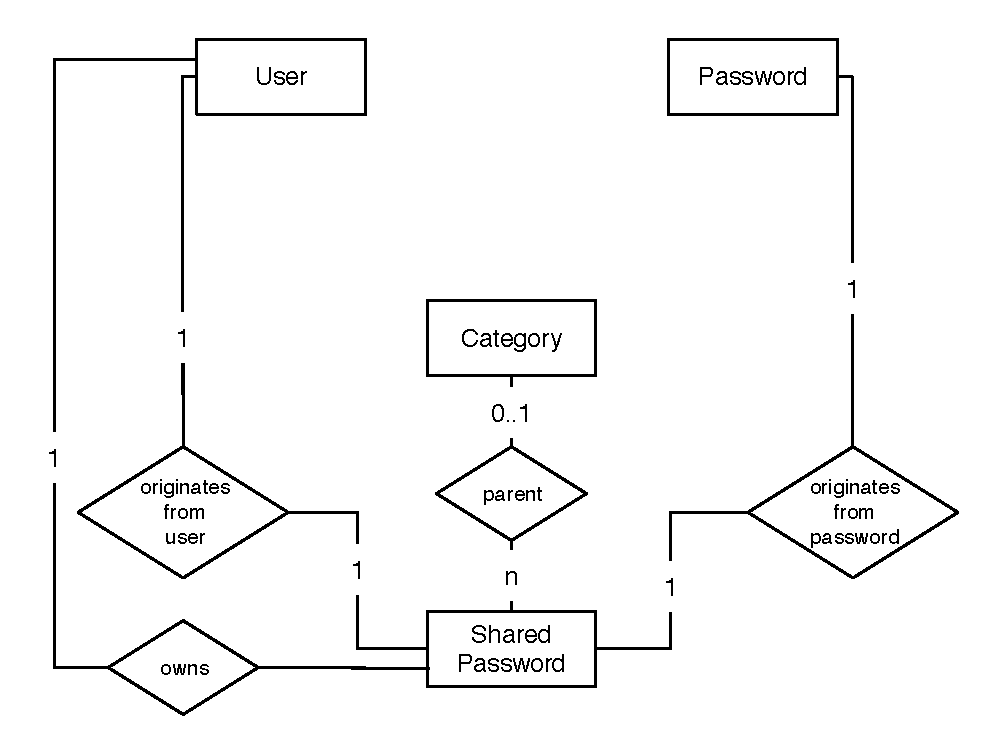
\includegraphics[scale=0.75]{figures/design/uml/erd/user-category-password-sharedpassword.eps}
				\caption{Shared Password's connections to the User, Password, and Category models.}
				\label{fig:relationship:sharedpassword}
			\end{figure}

		\subsection{The Invite Model}
			While the previous models have been very intertwined, the Invite model stands apart by quite a lot simpler. As has already been determined, the Invite model will need a UUID. Since this will, in the end, be part of an invite URL, this field is simply called the link. Furthermore, an expiration date will need to be stored, as it has been determined that the invite will only be valid, for 24 hours. As such, this \emph{very} simple model determined to contain the fields listed on table \ref{fig:model:invite} on page \pageref{fig:model:invite}. 
			
			\begin{table}[p]
				\centering
				\begin{tabular}{c|c}
					\textbf{Attribute} 		& \textbf{Type} 		\\
					ID 						& Unknown 		\\
					link  					& UUID \\
					expires 				& Unix timestamp \\
				\end{tabular}
				\caption{Fields of the Password model}
				\label{fig:model:invite}
			\end{table}

		\subsection{The Audit Model}
			Finally, there is the audit model. As described in section \ref{sec:audit} on page \pageref{sec:audit}, each entry should contain one of six actions. While this could easily be achieved using an enum, not all database technologies support this data structure. As such, an integer mapping is used. In practice, this means that each action is translated to an integer, before being stored. When retrieved, the same integer is used to generate the actual name of the action. This mapping is shown on figure \ref{table:audit:actionmapping} on page \pageref{table:audit:actionmapping}.

			What is a challenge when modelling these audit entries, is the reference to one of three things: Authentication attempts, passwords and shared passwords. Because it is a reference to multiple fields \emph{(the entry's target)}, a traditional database foreign key reference is simply not possible. As such, the reference will need to be stored in an integer \emph{(unfortunately loosing any restrictions from the relations, in the process)}. However, it is still needed to differentiate between an ID for a Password and for a Shared Password. As such, the targets type will need to be stored as well. Finally, as was decided previously, a hostname and a timestamp will need to be stored as well.

			\begin{table}[h!]
				\centering
				\begin{tabular}{r | l}
					\textbf{Action} 	& \textbf{Integer} 	\\
					\hline
					Create 				& 0 				\\
					Read 				& 1 				\\
					Update 				& 2 				\\
					Delete 				& 3 				\\
					Share 				& 4 				\\
					Success 			& 5 				\\
					Failure 			& 6 				\\					
				\end{tabular}
				\caption{Integer mapping of audit actions.}
				\label{table:audit:actionmapping}
			\end{table}

			\begin{table}[p]
				\centering
				\begin{tabular}{r|l}
					\textbf{Attribute} 		& \textbf{Type} 		\\
					ID 						& Unknown 	\\
					userId 					& User ID 	\\
					targetType 				& String 	\\
					targetId				& Integer 	\\
					action					& Integer 	\\
					time  					& Datetime 	\\
					host  					& String 	\\
				\end{tabular}
				\caption{Fields of the Audit model}
				\label{fig:model:audit}
			\end{table}

			As such, it is determined that the Audit model will contain the fields listed on table \ref{fig:model:audit} on page \pageref{fig:model:audit}. On figure \ref{fig:relationship:audit-user} on page \pageref{fig:relationship:audit-user}, the relationship between the Audit model and the Password and Shared Password models are depicted, with adjusted syntax to meet the slightly unique approach required for this model to work.
			
			\begin{figure}[p]
				\centering
				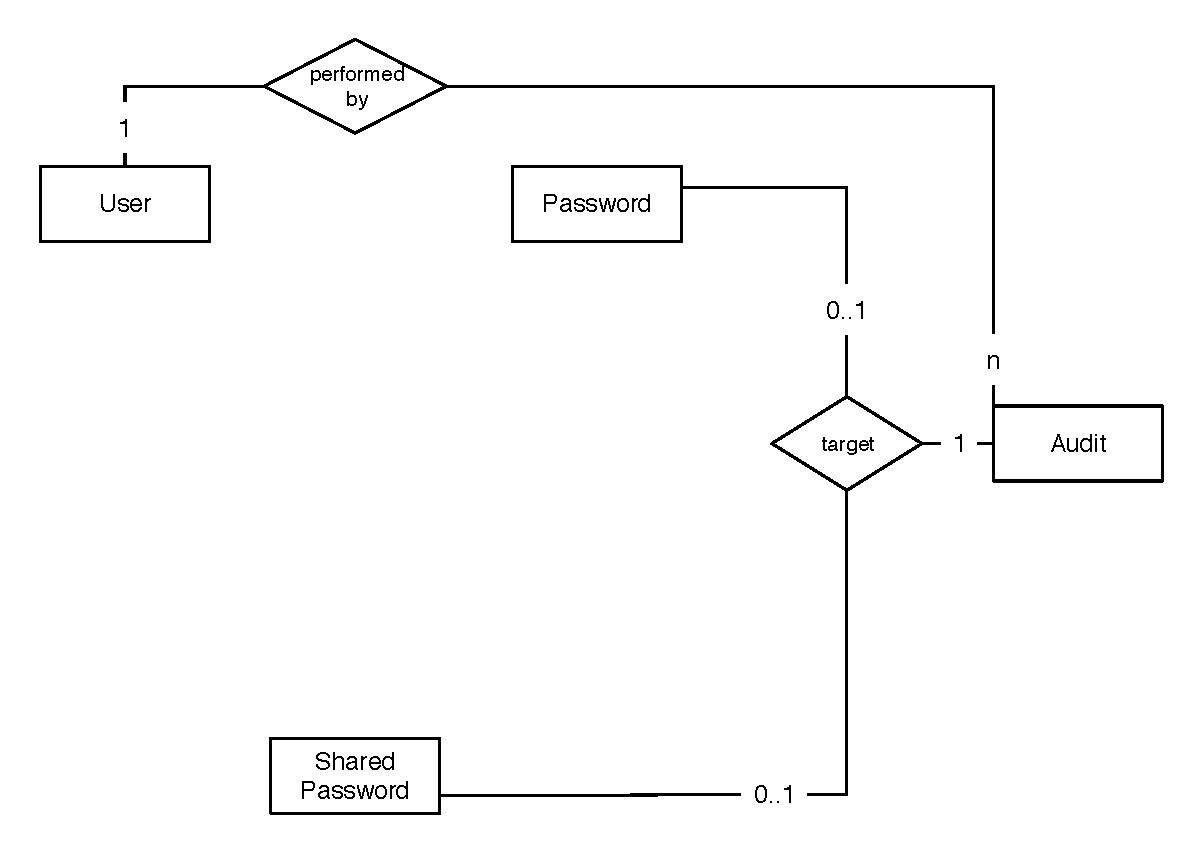
\includegraphics[width=\textwidth]{figures/design/uml/erd/audit-user-password-sharedpassword.eps}
				\caption{The Audit model's relationship with the User, Password, and Shared Password models.}
				\label{fig:relationship:audit-user}
			\end{figure}

		\subsection{Combining the Models}
			In the previous sections, the various models have been described and their relationships have been covered using Entity Relationship diagrams. Finally, all of these diagrams are combined into a single one, representing the entire system. This is found on figure \ref{fig:erd:full} on page \pageref{fig:erd:full}.

			\begin{figure}[p]
				\centering
				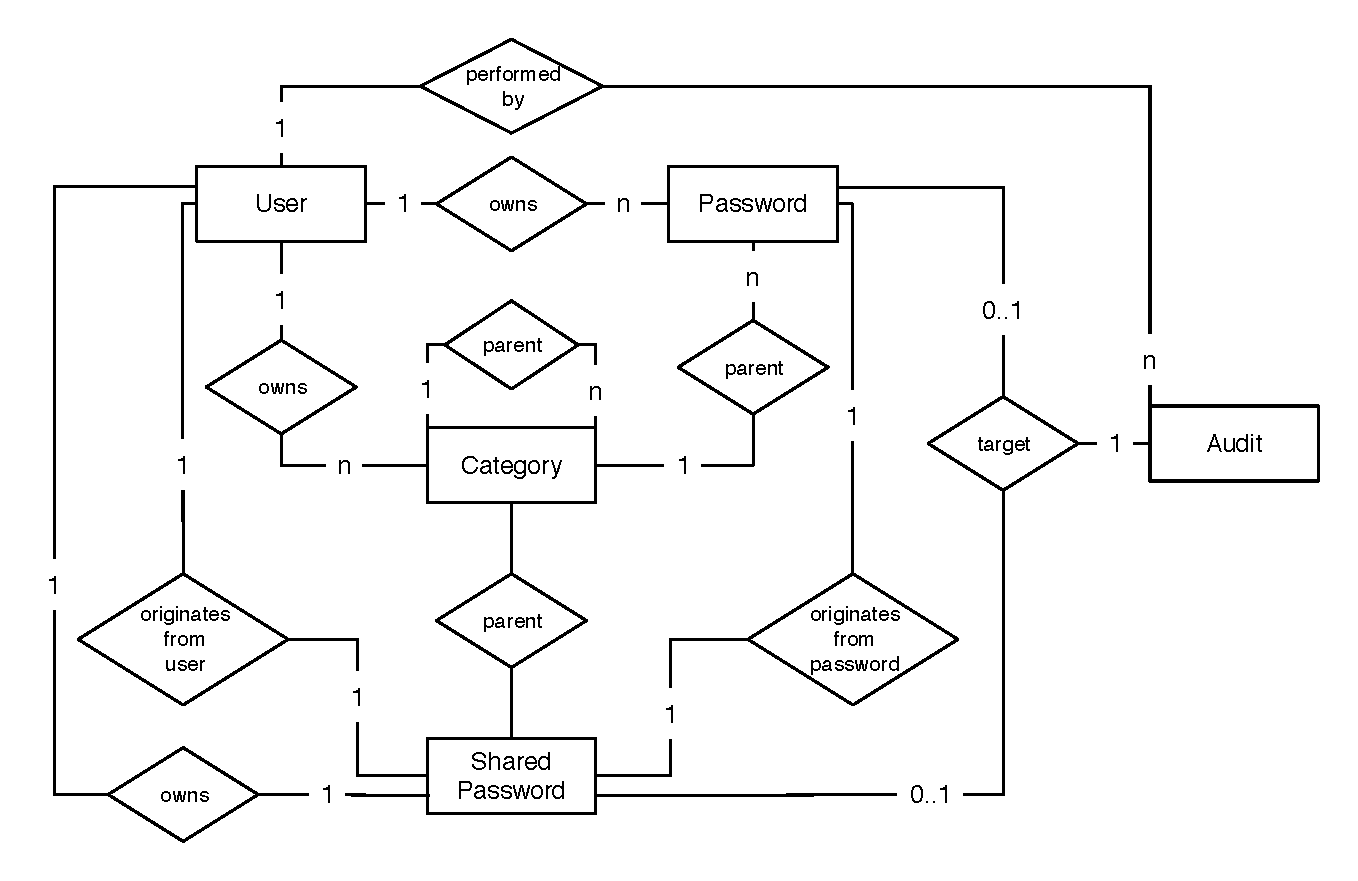
\includegraphics[width=\textwidth]{figures/design/uml/erd/complete.eps}
				\caption{Entity Relationship Diagram for the System, using Chen's notation.}
				\label{fig:erd:full}
			\end{figure}

		\subsection{Comparison With Requirements}
			\label{requirement:fulfilled:organization}
			\label{requirement:fulfilled:new}
			\label{requirement:fulfilled:retrieve}
			\label{requirement:fulfilled:delete}
			\label{requirement:fulfilled:entries}


			Section \ref{sec:model:category} on page \pageref{sec:model:category} introduced the concept of the Category model. This model allows for near infinite structuring of the password storage. As such, it is concluded that the solution fulfil functional requirement \#\ref{requirement:organization}:
			\vspace{-3ex}\begin{enumerate}
				\setlength\itemsep{0.1em}
				\setcounter{enumi}{4-1}
				\item Password organisation, multiple levels
			\end{enumerate}

			Additionally, section \ref{sec:model:password} on page \pageref{sec:model:password} described the model of each password entry. As such, it is concluded that the solution fulfil functional requirements \#\ref{requirement:new}, \#\ref{requirement:retrieve}, and \#\ref{requirement:delete}:
			\vspace{-3ex}\begin{enumerate}
				\setlength\itemsep{0.1em}
				\setcounter{enumi}{10-1}
				\item Support adding of new passwords
				\item Support retrieving stored passwords
				\item Support deleting stored passwords
			\end{enumerate}

			Finally, section \ref{sec:model:password:size} on page \pageref{sec:model:password:size} estimated the size of the database in regards to password entries, based on the approximated size of the password model. The conclusion was, that per $100.000$ entries in the database, it would take $145.6$ megabyte worth of storage, which in the modern world is no issue. As such, it is also concluded that the solution fulfil non-functional requirement \#\ref{requirement:entries}:
			\vspace{-3ex}\begin{enumerate}
				\setlength\itemsep{0.1em}
				\setcounter{enumi}{3-1}
				\item Support for \emph{at least} 100.000 password entries
			\end{enumerate}

	\section{Authorization}
		\label{sec:design:authorization}
		\todo{Describe authorization}

	\section{Storing the Data}
		\label{sec:database:type}
		Up until now the phrase ``database'' has been used as a generic description of persistent storage. In this section, this will be elaborated a bit. Generally speaking, there primarily exist two categories of databases: Relational Database Management Systems \emph{(RDBMSs)} and Non-SQL \emph{(NoSQL)}

		RDBMS/SQL is the oldest of the bunch. This category covers the first database schemes ever used, dating back to the 70's. This type of database has a very strict structure, compared to the others, requiring a structure of tables, which in turn contains columns. RDBMS are by far, the most used type of database, if for no other reason, that they've simply existed for a lot longer. Typically RDBMSs uses the Structured Query Language \emph{(SQL)}. An example of a RDBMS table can be seen on table \ref{fig:example:rldb} on page \pageref{fig:example:rldb}, consisting of columns ID, Username, and E-Mail, each entry has one value for each column. RDBMS often adhere to the ACID qualities: Atomic, Consistent, Isolated, and Durable. These ensures that either a query succeeds or it fails. Additionally, most implementations support transactions. Transactions work by effectively grouping several queries. The smart thing about this, is that either the transaction fails, or it succeeds. I.e. either all of the sub-queries succeeds, or if \emph{one} of them fails, all of the changes are rolled back.

		\begin{table}[h!]
			\centering
			\begin{tabular}{|c|c|c|}
				\hline
				\textbf{ID} 		& 	\textbf{Username} 		& \textbf{E-Mail} 		\\
				\hline
				1 					& Daniel 					& some@mail.com 		\\
				\hline
				2 					& John 						& someother@mail.com 	\\
				\hline
				3 					& Kylo Ren 					& kren@firstorder.com 	\\
				\hline
			\end{tabular}
			\caption{RDBMS table example}
			\label{fig:example:rldb}
		\end{table}

		While generally NoSQL is being used to describe a set of implementations, much like RDBMS is. However, this is not exactly true. There exists no standard for NoSQL databases, and each implementation varies greatly, which unfortunately results in the various implementations API's being vastly different from each other.

		NoSQL databases uses JSON format to represent information in the database. Where as SQL entries are restricted to the columns in the table, NoSQL does not have this constraint. The example from before, is stored as follows, using the JSON syntax. An example of this is found on listing \ref{lst:example:nosql} on page \pageref{lst:example:nosql}. One of the advantages of NoSQL is that since it does not have a strict schema, additional values can easily be added, for instance, it would be perfectly fine if a fourth user was added to the example, containing a field called phone. Where RDBMS adhere to ACID, NoSQL adhere to BASE: Basic Availability, Soft-state, and Eventual consistency.

		\begin{lstlisting}[style=json2,gobble=8, caption={NoSQL table example},label={lst:example:nosql}]
        [
            {
                "ID": 1,
                Username: Daniel,
                E-Mail: some@mail.com
            },
            {
                ID: 2,
                Username: John,
                E-Mail: someother@mail.com
            },
            {
                ID: 3,
                Username: Kylo Ren,
                E-Mail: kren@firstorder.com
            }
        ]
		\end{lstlisting}

		First and foremost, it is important to realise that \emph{all} of the technologies are capable of storing what is required. Having said that, one of the most credited advantages of NoSQL is their ability to scale horizontally. It can be spread out over multiple hosts, if need be. However, this project \emph{should} never reach that size. It is not intended to reach that size. As such, that advantage can be disregarded.

		At this point in time, tables such as \cite{db_rankings} could be used to argue that one type of database generally is faster. However, this really wouldn't matter much, in the context of this project. This is \emph{meant} to be self-hosted. It is \emph{meant} to be used by individuals. As such, it is \emph{highly} unlikely, that this project would ever find itself in a situation, where millions of records are being queried constantly. It would simply not make much sense, to use these arguments.

		But what then. In section \ref{sec:modelling} on page \pageref{sec:modelling}, the contents of the various models were discussed. The way it was designed, hints heavily at a underlying relational scheme. The audit entries, for instance, is a \emph{perfect} example of where a relational database would excel. Furthermore, there is the issue of invites. The process of using an invite would most likely involve something like the following steps:
		\begin{enumerate}
			\item Check that the invite exists
			\item Check that the invite is not expired
			\item Use the invite to create new user
			\item Delete invite
		\end{enumerate}
		However, as should be \emph{obvious} to everyone, this will be painfully vulnerable to race-conditions. This \emph{exact} scenario, is completely mitigated by the use of RDBMSs transactions: These would make the four steps atomic, in the eyes of the database. While some NoSQL databases adhering to the ACID principles, and supporting transactions, are starting to appear\cite{no_sql_transactions}, it is by far all of them that supports this.

		As such, it is decided that a more ``traditional'' RDBMS will be used for this solution.

		\subsection{Storage Schema}
			\todo{Create EER}

	\section{Ensuring Agnosticism}
		When creating a solution like this, it is important to make it as versatile as possible. As such, limiting it to run on a single platform only restricts deployment. As such, having an application that can run cross-platform is beneficial.

		\subsection{Platform Agnosticism}
			\label{sec:restrict:platform}
			As such, having a back-end being able to be run on the three major operating systems, would definitely be the best approach. These three operating systems are as follows:
			\begin{itemize}
				\item Windows
				\item OS X
				\item Linux
			\end{itemize}

			There exists numerous tools to develop such an API. Tools like Python and Ruby are just some some examples of languages, which makes cross-platform development a breeze.

			As such, a \emph{restriction} on the implementation is imposed: A language intended to work across multiple platforms is needed and should be used.

		\subsection{Database Agnosticism}
			\label{sec:restrict:database}
			While section \ref{sec:database:type} on page \pageref{sec:database:type} described why a RDBMS is better suited for this solution, it made no effort in selecting \emph{one} implementation \emph{(i.e. MySQL, MSSql etc.)}. This was very deliberately, partly because it is a question of implementation, and partly because restricting to \emph{one} implementation of database can be avoided.

			Using what is called a Database Abstraction Layer \emph{(DAL)} an application can work with the same type of databases, while not limiting itself to a \emph{single} solution. A DAL can ensure that the application can work with \emph{both} a separate MySQL database or a self-contained SQLite database, depending on configuration. This ensures that the user can customize the setup to work exactly how he or she wishes. 

			For instance, for a user running the solution on a single Raspberry Pi \emph{(see section \ref{sec:privatecloud_cost} on page \pageref{sec:privatecloud_cost})} a SQLite database would be be beneficial, due to the lower resource requirement. On the other hand, the user having an entire dedicated server at home -- already running a MySQL instance -- would probably prefer to combine it with his or her existing system.

			As such, using a DAL effectively ensures agnosticism when it comes to databases. Hence, another restriction on the implementation is imposed: The solution should use a DAL, ensuring compatibility with several database technologies.	

		\subsection{Comparison With the Requirements}
			\label{requirement:fulfilled:database}
			\label{requirement:fulfilled:platform}

			Having decided to introduce the restrictions described in sections \ref{sec:restrict:platform} and \ref{sec:restrict:database}, it is concluded that the solution now fulfil the functional requirements \#\ref{requirement:platform} and \#\ref{requirement:database}:
			\vspace{-3ex}\begin{enumerate}
				\setlength\itemsep{0.1em}
				\setcounter{enumi}{7-1}
				\item Platform agnostic
				\item Database agnostic
			\end{enumerate}

	\section{Licensing the Solution}
		\label{requirement:fulfilled:open-source}
		Finally, there is the issue of a software license. Since this project from day one, has been intended to be open-source, it only makes sense that the license reflects this. While many different licenses for this exact purpose exists, the most commonly used is the MIT license. This license essentially states that anyone can do whatever they want with the code, as long as they include the original copyright and license.

		The license used for this project, is found in appendix \ref{appendix:license}. As such, it is concluded that the solution fulfil the non-functional requirement \#\ref{requirement:open-source}:
		\vspace{-3ex}\begin{enumerate}
			\setlength\itemsep{0.1em}
			\setcounter{enumi}{2-1}
			\item Open Source License \emph{(MIT for instance)}
		\end{enumerate}


	\section{Final Comparison with the Requirements}
		In this chapter, a design for a solution has been proposed. It has been designed in a way, which makes it superior to not only the commercially available solutions, as found in section \ref{sec:solutions:commercial} on \pageref{sec:solutions:commercial}, but also the proposed academic solutions, found in section \ref{sec:solutions:academic} on page \pageref{sec:solutions:academic}. On figure \ref{table:requirements:final} on page \pageref{table:requirements:final}, a check list is found. This table references the requirements as specified in section \ref{sec:requirements} on page \pageref{sec:requirements}.

		As it is seen, all but two requirements are met. Functional requirement \#\ref{requirement:restart}:
		\vspace{-3ex}\begin{enumerate}
			\setlength\itemsep{0.1em}
			\setcounter{enumi}{17-1}
			\item Automatic start after a hardware reboot
		\end{enumerate}
		And non-functional requirement \#\ref{requirement:delay}:
		\vspace{-3ex}\begin{enumerate}
			\setlength\itemsep{0.1em}
			\setcounter{enumi}{7-1}
			\item A user should never wait more than maximum $500ms$ after any action in the user interface, before the changes take effect 
		\end{enumerate}

		First and foremost, non-functional requirement \#\ref{requirement:delay} is \emph{purely} a question of implementation. This is a requirement that is impossible to design ones way out of. As such, it merely transforms into a implementation \emph{restriction}, much in the likes of platform and database agnosticism \emph{(see sections \ref{sec:restrict:platform} and \ref{sec:restrict:database} on pages \pageref{sec:restrict:platform} and \pageref{sec:restrict:database}, respectively)}.

		This leaves but one requirement lacking: Functional requirement \#\ref{requirement:restart}. This is painfully easily achieved. Each of the major operating systems have their own service, intended for this \emph{specific} purpose. Linux has Upstart \emph{(legacy systems)} and Systemd \emph{(newer systems)}\cite{autostart:linux}, OS X has launchd\cite{autostart:osx}, and Windows supports creating a service from an executable file using the SC command\cite{autostart:windows}. Creating a script for each of these services is again, just a matter of implementation. Deployment of these scripts can be easily done using a simple shell or bash script.

		As such, it is finally concluded that the design is complete. As such, the implementation of the prototype will follow the descriptions and restrictions, found in this chapter.


		\begin{table}[h!]
			\begin{tabular}{r l c}
												& \rot{\textbf{Fulfilled}} 	& \rot{Section} \\
				\textbf{Functional} 			&						&					\\
				\hline
				\freq{item:distrib_password} 	& \green{\cmark} 			& \green{ \ref{requirement:fulfilled:distrib_password} }			\\
				\hline
				\freq{item:multi_user} 			& \green{\cmark} 			& \green{ \ref{requirement:fulfilled:multi_user} }			\\
				\hline
				\freq{item:admin_user} 			& \green{\cmark} 			& \green{ \ref{requirement:fulfilled:admin_user} }			\\
				\hline
				\freq{item:organization} 		& \green{\cmark} 			& \green{ \ref{requirement:fulfilled:organization} }			\\
				\hline
				\freq{item:sharing} 			& \green{\cmark} 			& \green{ \ref{requirement:fulfilled:sharing} }			\\
				\hline
				\freq{item:add} 			 	& \green{\cmark} 			& \green{ \ref{requirement:fulfilled:add} }			\\
				\hline
				\freq{item:platform} 			& \green{\cmark} 			& \green{ \ref{requirement:fulfilled:platform} }			\\
				\hline
				\freq{item:database} 			& \green{\cmark} 			& \green{ \ref{requirement:fulfilled:database} }			\\
				\hline
				\freq{item:passwords_local} 	& \green{\cmark} 			& \green{ \ref{requirement:fulfilled:passwords_local} }			\\
				\hline
				\freq{item:new} 				& \green{\cmark} 			& \green{ \ref{requirement:fulfilled:new} }			\\
				\hline
				\freq{item:retrieve} 			& \green{\cmark} 			& \green{ \ref{requirement:fulfilled:retrieve} }			\\
				\hline
				\freq{item:delete} 				& \green{\cmark} 			& \green{ \ref{requirement:fulfilled:delete} }			\\
				\hline
				\freq{item:audit} 				& \green{\cmark} 			& \green{ \ref{requirement:fulfilled:audit} }			\\
				\hline
				\freq{item:auth} 				& \green{\cmark} 			& \green{ \ref{requirement:fulfilled:auth} }			\\
				\hline
				\freq{item:change} 				& \green{\cmark} 			& \green{ \ref{requirement:fulfilled:change} }			\\
				\hline
				\freq{item:two-factor} 			& \green{\cmark} 			& \green{ \ref{requirement:fulfilled:two-factor} }			\\
				\hline
				\freq{item:restart} 			& \red{\xmark} 			& \red{ \ref{requirement:fulfilled:restart} }			\\
				\hline
				\textbf{Non-Functional} 		&  			 			& 					\\
				\hline
				\nfreq{item:user_storage} 		& \green{\cmark} 			& \green{ \ref{requirement:fulfilled:user_storage} }			\\
				\hline
				\nfreq{item:open-source} 		& \green{\cmark} 			& \green{ \ref{requirement:fulfilled:open-source} }			\\
				\hline
				\nfreq{item:entries} 			& \green{\cmark} 			& \green{ \ref{requirement:fulfilled:entries} }			\\
				\hline
				\nfreq{item:encryption} 		& \green{\cmark} 			& \green{ \ref{requirement:fulfilled:encryption} }			\\
				\hline
				\nfreq{item:comms} 				& \green{\cmark} 			& \green{ \ref{requirement:fulfilled:comms} }	\\
				\hline
				\nfreq{item:tls1.2} 			& \green{\cmark} 			& \green{ \ref{requirement:fulfilled:tls1.2} }			\\
				\hline
				\nfreq{item:delay} 				& \red{\xmark} 			& \red{ \ref{requirement:fulfilled:delay} }			\\
				\hline
			\end{tabular}
			\caption{Requirements from section \ref{sec:requirements} on page \pageref{sec:requirements}, and where in this chapter they are concluded to be fulfilled.}
			\label{table:requirements:final}
		\end{table}
%%\chapter{What Could Go Wrong?}
\chapter{Risks}
	Having described the implementation of the prototype, it is very important to acknowledge any short-comings or dangers in the use of the final solution. As such, in this chapter the greatest risks are discussed.
	

	\section{Weak Authentication and Decryption Passwords}
		One of the most fundamental risks of using this implementation, is if the user chooses a weak password. Granted, this is a weakness that applies to \emph{everything} protected by a weak password.

		If a can be guessed easily, by known publicly available information regarding the user, or can be bruteforced in a reasonable short about of time, they are thought to be weak. Such a password would in the event of an attacker attempting to gain access, result in greater risk of leaking the \emph{actual} passwords.

		Unfortunately, preventive measures for this type of weakness, is fairly useless. Enforcing password policies is how it is often done in critical systems, but more often than not, the resulting password is chosen so it is easy to remember. As such, it is decided that this risk is \emph{completely} up to the user to avoid.

	\section{Identical Encryption and Decryption Passwords}
		In section \ref{sec:design:pseudo-zero-knowledge} on page \pageref{sec:design:pseudo-zero-knowledge} it was discussed why the design of the system requires two passwords. However, at \emph{no} point will the implementation ever actually compare these passwords. As such, it is \emph{completely} possible for the user to have identical authentication and decryption passwords.

		The risk of this, is potentially giving the server owner the ability to decrypt the stored passwords, since the authentication password \emph{is} sent to the back-end, for authentication purposes. However, this all depends on the user's \emph{choice}, and as such is not regarded as a critical risk.
	
	\section{Trusting the Server Owner}
		While the pseudo-zero-knowledge concept introduced in section \ref{sec:design:pseudo-zero-knowledge} on page \pageref{sec:design:pseudo-zero-knowledge} is intended to keep admins from reading all of the users' passwords, there is more to the story.

		The admin, whom is assumed to be the owner of the back-end, \emph{could} change the JavaScript files of the front-end, making them send all the unencrypted data back to him. 

		In \emph{theory} this could be mitigated by publishing a checksum of the bundled JavaScript file, that the front-end executes. This could then be compared, using a separate browser plugin on load, determining whether or not the file had been tampered with.

		However, there is a much more fundamental issue here: Trust. This implementation is meant to be \emph{self-hosted}. The multi-user support is intended to allow multiple users from the same small community or home, e.g. husband and wife, to share the same back-end for storing their private passwords. As such, a certain level of \emph{trust} is assumed. The pseudo-zero-knowledge ensures that the admin can not read the passwords, using information found in the implementation as originally developed. Beyond that, the users will simply have to trust the admin, that he or she will not deliberately alter the files, in order to access their passwords.

	\section{Third Party Libraries}
		As previously stated, the implementation relies on third party libraries, to perform certain functions. For instance, the Forge library is used for handling encryption in the front-end, and the Node-Argon2 library, is used for performing Argon2 password hashing in the back-end. 

		Using these libraries -- or dependencies, as they're called in the Node.js community -- enabled prototypes to be rapidly developed. However, they also introduce a risk: The implementation relies on other people's code. Recently the largest dependency manager for Node.js, npm, experienced a catastrophic event. A very basic package, \verb=left-pad= was removed from npm, due to a legal dispute between the author and a third party\cite{npm_leftpad}. This caused a chain reaction of chaos, as packages that depended on \verb=left-pad= no longer could be installed, and packages depending on those packages couldn't either -- and so forth. This is unfortunately the risk, when working with these kinds of dependencies, but it isn't even the worst.

		When depending on libraries, the developer\emph{(s)} trust that the author\emph{(s)} of the library is forthright about the content of the library. For instance, the Forge library could, for all intents and purposes, simply send every single encryption payload to a remote server. Luckily, since this \emph{is} the world of open source, the source code can be inspected, and security flaws and vulnerabilities possibly found. However, there \emph{might} still be both intentional and unintentional security risks involved with using these libraries. As such, it is the developers duty to assess the quality of \emph{any} dependency used.

	\section{Dumping the Memory}
		Unfortunately, since the implementation is run in a browser, it is not possible to implement features depending on for instance Microsoft's Data Protection Application Programming Interface \emph{(DPAPI)}, like KeePass does. As such, storing the passwords unencrypted is \emph{unfortunately} a security risk.

		There really isn't any way around this risk. For it to be shown to the user, in the browser, it needs to be decrypted. For it to be shown, it needs to be stored. Should an attacker make a dump of the process memory, he or she will \emph{unfortunately} gain access to any passwords decrypted. 

		The same is said about swap partitions and pagefiles. Unfortunately, there is a risk of clear text passwords ending up in these. It is a risk that comes with the choice of implementation. Should it have been chosen to implement native clients instead, this could possibly be circumvented. So this risk, is the price that will have to be paid, for the convenience of a web application.

		Even the encrypted passwords are somewhat at risk. For user experience purposes, the decrypted private key is kept in memory. A mechanism clearing this variable could of course be devised, but that would result in the user having to enter their decryption password \emph{every} time he or she needed to access a password -- which would result in a horrible user experience.


		%So even when removing the decrypted passwords, the encryption key for decrypting \emph{all} passwords, still resides \emph{in memory}. One could of course go about clearing this as well, but that would mean the user would have to enter the decryption password \emph{every} time he or she needed to access a password -- which would result in a horrible user experience.

		%The only redeeming thing to be said about this risk, is the fact that the implementation attempts to remove decrypted passwords again, as soon as possible. When the user changes focus from the password, its variable is overwritten. This is, however, doesn't increase the security all that much. For user experience purposes, the decrypted private key is kept in memory. So even when removing the decrypted passwords, the encryption key for decrypting \emph{all} passwords, still resides \emph{in memory}. One could of course go about clearing this as well, but that would mean the user would have to enter the decryption password \emph{every} time he or she needed to access a password -- which would result in a horrible user experience.

		All in all, this risk is unfortunately unavoidable. It is simply the price paid for the convenience.
	
	\section{Loss of Data in the Database}
		As much as we wish they were, harddrives, flash cards, and USB sticks are fallible. Drive failures \emph{can} -- and eventually \emph{will} -- happen. Unfortunately, not all users will run with a setup supporting parity checks. As such, backing up the database every so often is very much \emph{encouraged}. While this will \emph{not} completely mitigate the threat of data loss, it minimizes the damage done in such an event.

		Backing up the database can easily be done with a cronjob \emph{(or similar)}.

	\section{Leaking the Token}
		In section \ref{sec:design:jwt} on page \pageref{sec:design:jwt} it was decided that the implementation will be using JWT's to handle API authentication. What was \emph{not} discussed, was the security impact this would have.

		When JWTs are used, commonly there is an expiration time set. At the time of this writing, that timer is set to 24 hours, meaning that 24 hours after issuing, the token is no longer valid. As such, after the token is expired the user will need to re-authenticate to access the back-end again.

		However, that also means that should this token fall into the hands of the attacker, he or she will have access to the user's data for 24 hours. This would allow an attacker to change and delete passwords at will, but since password encryption and decryption happens in the browser, he or she will \emph{not} have direct access to the passwords. Avoiding the loss of passwords, can be somewhat mitigated, by backing up the database, as described in the previous section.

		Obtaining these tokens commonly happen through either Cross-Site Request Forgery \emph{(CSRF)} or Cross-Site Scripting \emph{(XSS)}. While there definitely could be security vulnerabilities not found at this point, it is believed that no such exists. Additionally, it is not possible to intercept the token in transit, due to HTTPS being enforced at \emph{all} times.

		As such, the risk of the token being compromised, is relatively low.

		%Another option is to allow for token revocation. This would entail storing the token in the database, allowing the user to revoke tokens at any point in time.


	\section{Forgetting the Password}
		One of the more unfortunate ``issues'' with the implementation, is the lack of account recovery. The authentication password can, \emph{of course}, be reset. But the decryption password can \emph{not} be reset -- for good reasons. As such, if the user forgets his or her decryption password, \emph{nothing} can be done.

		Should this situation arise, it would be unfortunate. But there is nothing that can be done to remedy this risk, that would not lower the overall security of the system. As such, it is deemed a necessary risk.

	\section{Summing Things Up}
		In the previous sections various risks of running the system has been introduced. These range from trusting the owner of the setup, to depending on third party libraries.




		Taken all the risks into consideration, it is still deemed better to deploy the solution as is, rather than trusting remote services with ones password data.

\chapter{Implementing the System: The Back-End}
	In chapter \ref{chap:design} the design of the solution was described. This description ranged from overall specifications, to more detailed model designs. In the following two chapters the implementation of a \emph{prototype}, following the design specifications from chapter \ref{chap:design}, is described.

	To achieve the best possibly experience for the reader, the description is split into two parts: The back-end and the front-end. In \emph{this} chapter, the implemenation of the prototype back-end is described.


	\section{The Language of the Back-End}
		\subsection{Python}
			One of the more popular languages for self-hosted software is Python. Combined with frameworks such as Django or Flask, it acts as a very powerful way to develop a web API.




		\subsection{Ruby}
		\subsection{Node.js}
		\subsection{C\#}
		\subsection{PHP}
		\subsection{C++}

	\section{To Framework or Not To Framework}
		\subsection{Express}
		\subsection{Hapi}
		\subsection{Restify}
		\subsection{Koa}


	\section{Database Abstraction Layer}
		As decided in section \ref{sec:restrict:database} on page \pageref{sec:restrict:database}, a database abstraction layer is necessary. While Object-Relational Mapping \emph{(ORM)} strictly speaking isn't the same as a DAL, for this section the two are considered equivalent.

		The two most widely used solutions for this, is Sequelize, Bookshelf, and Knex \emph{(Bookshelf is built ontop of Knex)}. Sequelize and Bookshelf are both ORMs, whereas Knex is a DAL. In regards to platform support, they are fairly similar. Sequelize supports PostgreSQL, MySQL, SQLite and MSSQL. Bookshelf/Knex supports MySQL, SQLite, Postgres, MariaDB, and Oracle.

		While working with ORMs generally takes database interactions to a higher abstraction level, it is thought that this also removes certain insight into how some queries work. Additionally, Knex's chainable methods, makes for query building in the style of Javascript promises. As such, it is concluded the Knex is the superior choice as a DAL for the implementation.

	\section{API Endpoints}
		\label{sec:api}
		Before defining the endpoints, the resources \emph{(see section \ref{sec:design:rest} on page \pageref{sec:design:rest})} of the application need to be determined. Looking at the models defined in section \ref{sec:modelling} on page \pageref{sec:modelling}, these offer a great starting point for resources.


		\subsection{The Users Resource}
			First and foremost there is the collection of Users. This collections represents the user base as a whole. \verb=POST=ing to this collection, would by extension mean the creation of a new user. \verb=GET=ing the user collection, mean retrieving all user entries, with their username and other attributes in the ``public domain''. \verb=PUT= and \verb=DELETE= is slightly different. They're used for updating and deleting a \emph{single} user, in the entire collection. As such, the endpoint needs to have a user ID postfixed. Adhering to the standard, \emph{all} API endpoints will have \verb=/api= prefixed. These API endpoints are listed on table \ref{tab:api:users} on page \pageref{tab:api:users}.

		\subsection{The Passwords Resource}
			Then there is the collection of passwords. However, there is a slight caveat when it comes to this collection. Since each password is \emph{owned} by a user, it can generally be thought that there exists \emph{multiple} collection -- one for each user. As such, the password collection is gated behind the user resource and the ID specifying exactly which user owns said password. The same approach to designing these endpoints are used, as with the user resource and the result of this is found on table \ref{tab:api:passwords} on page \pageref{tab:api:passwords}.

			For simplicity's sake, access to shared passwords are gated behind the passwords resource. As such, a collection called shares -- which belongs to a specific password -- denotes the collection of users this specific password has been shared to. Additionally, two collections are added as well: \verb=shared= and \verb=shares=. These two are  \emph{very} similar in name, which unfortunately might result in some confusion. The \verb=shares= resource denotes passwords shared \emph{to} the user and the \verb=shared= resource denotes passwords that the user has shared to \emph{others}. These endpoints are found on table \ref{tab:api:sharedpasswords} on page \pageref{tab:api:sharedpasswords}.

		\subsection{The Categories Resource}
			The same argument made in regards to the passwords collection, can be said about categories. Each user has their own private password collection, which is -- similar to passwords -- gated behind the owning user's ID. This can be seen on table \ref{tab:api:categories} on page \pageref{tab:api:categories}.

		\subsection{The Invites Resource}
			When an admin creates a new invites, it can be said he \verb=POST=s it to the invites resource. \verb=GET=ing an ID, returns the status of an ID stored in the database. Then, there is finally the act of using an invite. Since a user is created, it only makes sense that the \verb=POST= method is needed. However, since the regular endpoint is already being posted to, an additional endpoint is needed. As such, appending the endpoint with \verb=/accept= will achieve this. This can be seen on table \ref{tab:api:invites} on page \pageref{tab:api:invites}.

		\subsection{The Audit Resource}
			The Audit resource is actually very simple. It only consists of a single endpoint; Getting the audit log. Since this resource is owned by individual users, this is -- much like passwords and categories -- gated behind the user collection and a specific ID. This can be seen on table \ref{tab:api:audit} on page \pageref{tab:api:audit}.

		\subsection{The Auth Resource}
			\label{sec:api:auth}
			The Auth resource is a little bit more interesting. Of course, there is the generic \verb=POST=, containing the user's username and password, for authentication purposes. The details of this is covered in section \ref{sec:design:authentication} on page \pageref{sec:design:authentication}. However, this is not all. Since the solution supports TOTP two-factor-authentication, as described in section \ref{sec:mfa} on page \pageref{sec:mfa}, endpoints for enabling this is needed as well. In section \ref{sec:design:breaking-rest} on page \pageref{sec:design:breaking-rest} it was argued that at one point it was \emph{necessary} to break the REST principles. As such, two endpoints are needed: One for generating a new secret and caching it, and one for actually verifying said secret. 


		
		\newcolumntype{L}[1]{>{\hsize=#1\hsize\raggedright\arraybackslash}X}%
		\newcolumntype{R}[1]{>{\hsize=#1\hsize\raggedleft\arraybackslash}X}%
		\newcolumntype{C}[2]{>{\hsize=#1\hsize\columncolor{#2}\centering\arraybackslash}X}%
		
		\begin{table}
			\definecolor{tablerow1}{RGB}{230,230,230}
			\definecolor{tablerow2}{RGB}{255,255,255}
			\rowcolors{2}{tablerow1}{tablerow2}
			
			\begin{tabularx}{\textwidth}{ R{0.2} | L{0.6} | L{0.2} }
				\bfseries Method & \bfseries Endpoint & \bfseries Description% specify table head
				\csvreader[head to column names]{resources/api/users.csv}{}% use head of csv as column names
				{\\\hline\method & \texttt{\endpoint} & \description}% specify your coloumns here
			\end{tabularx}

			\caption{API endpoints for the Users resource.}
			\label{tab:api:users}
		\end{table}


		\begin{table}
			\definecolor{tablerow1}{RGB}{230,230,230}
			\definecolor{tablerow2}{RGB}{255,255,255}
			\rowcolors{2}{tablerow1}{tablerow2}
			
			\begin{tabularx}{\textwidth}{ R{0.2} | L{0.6} | L{0.2} }
				\bfseries Method & \bfseries Endpoint & \bfseries Description% specify table head
				\csvreader[head to column names]{resources/api/passwords.csv}{}% use head of csv as column names
				{\\\hline\method & \texttt{\endpoint} & \description}% specify your coloumns here
			\end{tabularx}

			\caption{API endpoints for the Passwords resource.}
			\label{tab:api:passwords}
		\end{table}

		\begin{table}
			\definecolor{tablerow1}{RGB}{230,230,230}
			\definecolor{tablerow2}{RGB}{255,255,255}
			\rowcolors{2}{tablerow1}{tablerow2}
			
			\begin{tabularx}{\textwidth}{ R{0.2} | L{0.6} | L{0.2} }
				\bfseries Method & \bfseries Endpoint & \bfseries Description% specify table head
				\csvreader[head to column names]{resources/api/sharedPasswords.csv}{}% use head of csv as column names
				{\\\hline\method & \texttt{\endpoint} & \description}% specify your coloumns here
			\end{tabularx}

			\caption{API endpoints for accessing Shared Passwords.}
			\label{tab:api:sharedpasswords}
		\end{table}		

		\begin{table}
			\definecolor{tablerow1}{RGB}{230,230,230}
			\definecolor{tablerow2}{RGB}{255,255,255}
			\rowcolors{2}{tablerow1}{tablerow2}
			
			\begin{tabularx}{\textwidth}{ R{0.2} | L{0.6} | L{0.2} }
				\bfseries Method & \bfseries Endpoint & \bfseries Description% specify table head
				\csvreader[head to column names]{resources/api/categories.csv}{}% use head of csv as column names
				{\\\hline\method & \texttt{\endpoint} & \description}% specify your coloumns here
			\end{tabularx}

			\caption{API endpoints for the Categories resource.}
			\label{tab:api:categories}
		\end{table}
		
		\begin{table}
			\definecolor{tablerow1}{RGB}{230,230,230}
			\definecolor{tablerow2}{RGB}{255,255,255}
			\rowcolors{2}{tablerow1}{tablerow2}
			
			\begin{tabularx}{\textwidth}{ R{0.2} | L{0.6} | L{0.2} }
				\bfseries Method & \bfseries Endpoint & \bfseries Description% specify table head
				\csvreader[head to column names]{resources/api/invites.csv}{}% use head of csv as column names
				{\\\hline\method & \texttt{\endpoint} & \description}% specify your coloumns here
			\end{tabularx}

			\caption{API endpoints for the Invites resource.}
			\label{tab:api:invites}
		\end{table}

		\begin{table}
			\definecolor{tablerow1}{RGB}{230,230,230}
			\definecolor{tablerow2}{RGB}{255,255,255}
			\rowcolors{2}{tablerow1}{tablerow2}
			
			\begin{tabularx}{\textwidth}{ R{0.2} | L{0.6} | L{0.2} }
				\bfseries Method & \bfseries Endpoint & \bfseries Description% specify table head
				\csvreader[head to column names]{resources/api/audit.csv}{}% use head of csv as column names
				{\\\hline\method & \texttt{\endpoint} & \description}% specify your coloumns here
			\end{tabularx}

			\caption{API endpoint for the Audit resource.}
			\label{tab:api:audit}
		\end{table}

		\begin{table}[p]
			\definecolor{tablerow1}{RGB}{230,230,230}
			\definecolor{tablerow2}{RGB}{255,255,255}
			\rowcolors{2}{tablerow1}{tablerow2}
			
			\begin{tabularx}{\textwidth}{ R{0.2} | L{0.6} | L{0.2} }
				\bfseries Method & \bfseries Endpoint & \bfseries Description% specify table head
				\csvreader[head to column names]{resources/api/auth.csv}{}% use head of csv as column names
				{\\\hline\method & \texttt{\endpoint} & \description}% specify your coloumns here
			\end{tabularx}

			\caption{API endpoints for the Auth resource.}
			\label{tab:api:auth}
		\end{table}

	\section{Workaround To Be Self-Contained}
		Unfortunatly, Restify's documentation is sometimes lackluster. They have what they call the serveStatic method. From their decription, its intended use is to deliver a default file, if a match is not found. This is exactly what is needed for the front-end's router \emph{(more on this in section \ref{sec:impl:ui-router} on page \pageref{sec:impl:ui-router})}. However, after much fiddling, it was found simply not to work.

		As such, a workaround is needed. After having stated the API routes, six new routes are defined as is seen on table \ref{tab:api:workaround} on page \pageref{tab:api:workaround}. This ensures that any API hits are given the proper error code, while ensuring that the application for the front-end is being delivered in all cases.
		\begin{table}
			\centering
			\begin{tabular}{r | l}
				\textbf{Method} & \textbf{Endpoint} \\
				\hline
				\verb=GET=		& \verb=/api/.*= \\
				\verb=HEAD=		& \verb=/api/.*= \\	
				\verb=POST=		& \verb=/api/.*= \\	
				\verb=PUT=		& \verb=/api/.*= \\
				\verb=DEL=		& \verb=/api/.*= \\
				\verb=PATCH=	& \verb=/api/.*= \\	
			\end{tabular}
			\caption{Workaround error routes, to make the API adhere to standards and the front-end's router to work \emph{(see section \ref{sec:impl:ui-router} on page \pageref{sec:impl:ui-router})}}
			\label{tab:api:workaround}
		\end{table}
		%RESTIFY workaround with serve static

	\section{Authentication}
		In section \ref{sec:api:auth} on page \pageref{sec:api:auth} the endpoints involved in authentication was described. In this section, the process is described a little further. 

		As with any authentication, the user starts by sending his or her username and password \emph{(see section \ref{sec:design:authentication} on page \pageref{sec:design:authentication})}. If two factor authentication is not enabled, the standard verification approach is made. If the password matches, http code \verb=200= is returned, signifying successful authentication. Should it not match, http code \verb=401= is returned, signifying unsuccessful authentication. All in all, very basic.

		Should two factor authentication be enabled, however, a more complex event happens. Since the front-end won't know if two factor authentication is enabled or not, this needs to be conveyed to the front-end. As such, should the user have two-factor authentication enabled, but the token is missing from the body, http error code \verb=403= is returned. \verb=403= is defined as follows, by RFC2616\cite{httpcodes}:
		\begin{citequote}[sec.10.4.4]{httpcodes}
			   The server understood the request, but is refusing to fulfill it...
		\end{citequote}
		When the front-end receives the \verb=403= from the authentication endpoint, it \emph{knows} to promt to the user for a two-factor-token. Once this token is obtained, the request is sent again -- with the new token. Once received, the back-end verifies the password, similar to before, and verifies that the token is correct. If all fields are vitrified the back-end responds with \verb=200= to signify successful authentication. Should both fields not be verified, the response is \verb=401= to signify unsuccessful authentication. Figure \ref{fig:sequence:auth} on page \pageref{fig:sequence:auth} depicts this series of event, in a sequence diagram.

		\begin{figure}[p]
			\centering
			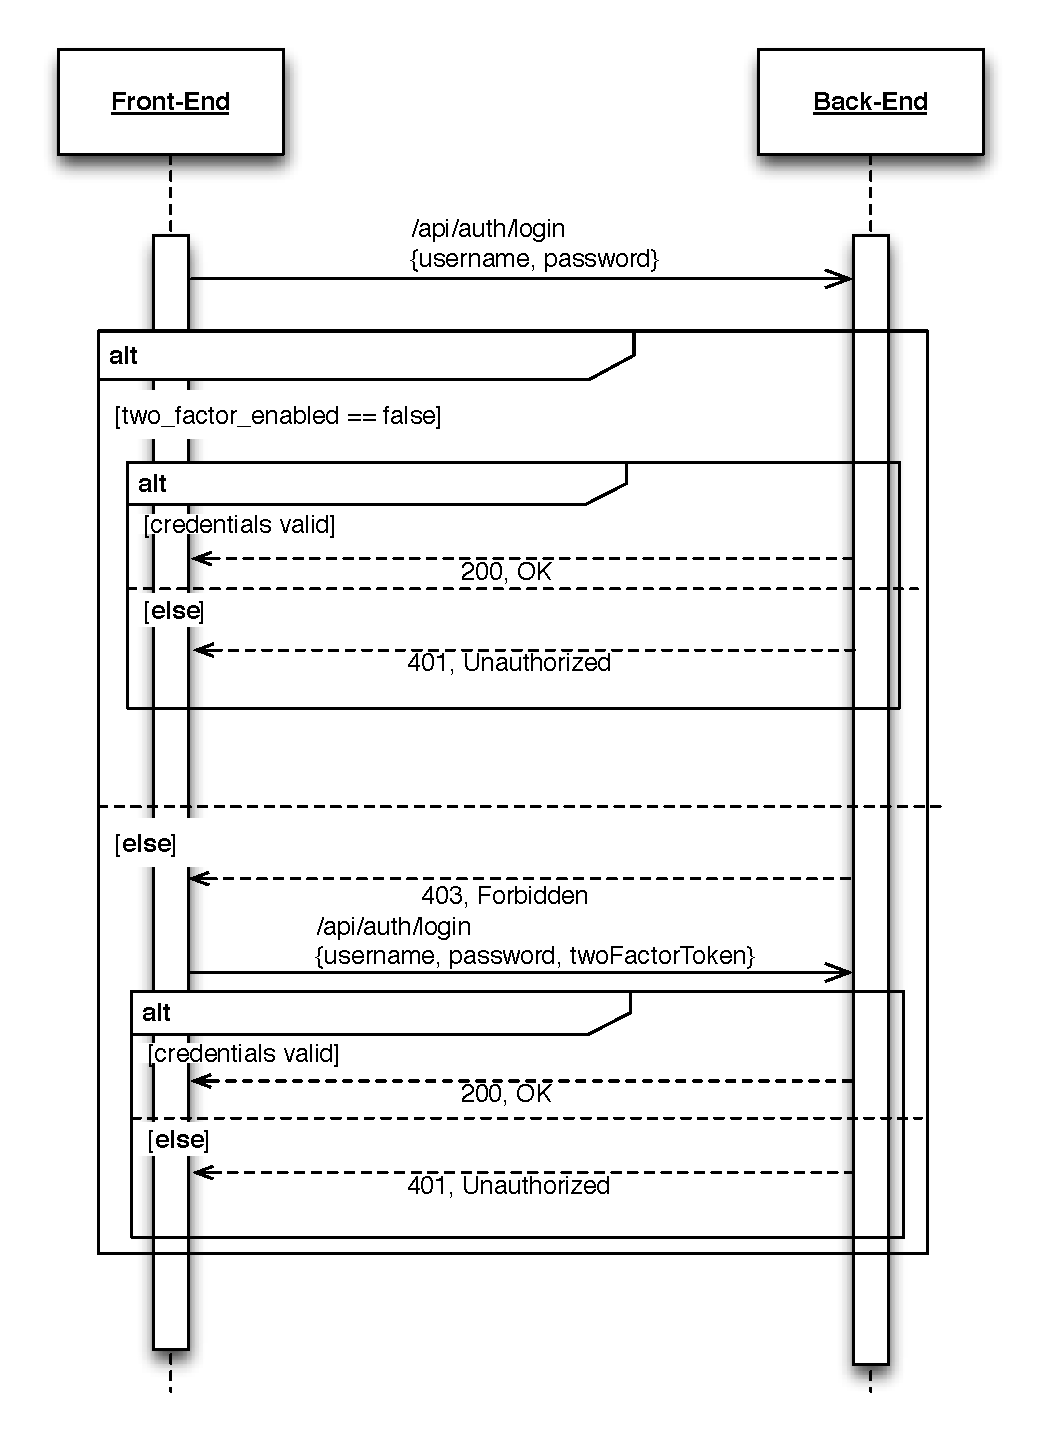
\includegraphics[width=0.8\textwidth]{figures/implementation/uml/sequence/authentication.eps}
			\caption{Sequence diagram showing the process of how the front-end authenticates to the back-end.}
			\label{fig:sequence:auth}
		\end{figure}

	\section{Authorization}
		For authorization purposes two strategies will be used: Simple and advanced. For all purposes where the simple is a possibility, it will be used. In section \ref{sec:design:authorization} on page \pageref{sec:design:authorization} it was described which users has access to which entities. The following two sections will adhere to this design.

		\subsection{Basic Authorization}
			Using the API described in section \ref{sec:api} on page \pageref{sec:api}, it is clearly seen that models' IDs are found in the URL. As such, using the owner field, of these models, it can easily be determined if the authenticated user has access to any given resource.

			As per the design, \emph{both} the user and admins will have full access to all user methods. This is simply handled with a comparison:
			\begin{lstlisting}[gobble=16,language=JavaScript]
                if( req.resolved.user.id === user.id || req.resolved.user.isAdmin ){
			\end{lstlisting}

			Since it is only the user self, that has access to his or her passwords, this is also handled extremely easy by doing:
			\begin{lstlisting}[gobble=16,language=JavaScript]
                if( password.owner === user.id && user.id === req.resolved.user.id ){
			\end{lstlisting}
			The exact same is done for categories:
			\begin{lstlisting}[gobble=16,language=JavaScript]
                if( category.owner === user.id && user.id === req.resolved.user.id ){
			\end{lstlisting}

			Shared passwords however, are a little bit more difficult. As has already been stated, both the user \emph{sharing} the password and the user receiving the shared password needs access to this resource. As such, the logic is a little different:
			\begin{lstlisting}[gobble=16,language=JavaScript]
                if( (share.owner === user.id && user.id === req.resolved.user) || (share.origin_owner === user.id && user.id === req.resolved.user)){
			\end{lstlisting}
		
			If the above snippets are evaluated to \verb=true=, the code keeps executing. If it is evaluated to false, the back-end returns http code \verb=403=, Forbidden denoting that the user does \emph{not} have sufficient privileges to access that specific data.

		\subsection{Advanced Authentication}

	\section{Dependencies}


\chapter{Implementing the System: The Front-End}
	\section{Developing for the Browser}
		\subsection{Flash}
		\subsection{Java}
		\subsection{Javascript}
		\subsection{Silverlight}


	\section{Using a Framework}
		\begin{itemize}
			\item Angular 1.5
			\item Angular 2.0
			\item ReactJS
			\item Ember
			\item Polymer
		\end{itemize}


	\section{UI-Router}
		\label{sec:impl:ui-router}

	\section{Performing Encryption}

	\section{Generating Passwords}


	
	\section{Resolving Objects}
		restify middelware automaticly get objects from storage




\newpage
\chapter{Todos}
\todos



\appendix
\chapter{Java Remote Method Invocation Snippets}
\label{appendix:rmi}

\lstinputlisting[
	frame=single,
	caption={UserService Interface},
	language=Java,
	breaklines=true,
	]{snippets/rmi/UserService.java}

\lstinputlisting[
	frame=single,
	caption={UserService Server},
	language=Java,
	breaklines=true,
	]{snippets/rmi/UserServiceImpl.java}

\lstinputlisting[
	frame=single,
	caption={Client using the UserService},
	language=Java,
	breaklines=true,
	]{snippets/rmi/Client.java}

\chapter{Software License}
\label{appendix:license}
\lstinputlisting[language={}]{snippets/LICENSE}
\chapter{API}

	\definecolor{tablerow1}{RGB}{230,230,230}
	\definecolor{tablerow2}{RGB}{255,255,255}
	\rowcolors{2}{tablerow1}{tablerow2}
	
	\begin{tabularx}{\textwidth}{ R{0.2} | L{0.6} | L{0.2} }
		\bfseries Method & \bfseries Endpoint & \bfseries Description% specify table head
		\csvreader[head to column names]{resources/api.csv}{}% use head of csv as column names
		{\\\hline\method & \texttt{\endpoint} & \description}% specify your coloumns here
	\end{tabularx}

%\chapter{Stuff and Things}

This appendix is full of stuff ...
%-----------
% Backmatter
%-----------
\backmatter
\chaptermark{Bibliography}
\renewcommand{\sectionmark}[1]{\markright{#1}}
\sectionmark{Bibliography}
\addcontentsline{toc}{chapter}{Bibliography}        %Force addition of Bibliography to TOC
\bibliographystyle{alpha}                           %Use alpha codes for references
\bibliography{references,references/images.bib,references/techpapers.bib,references/design.bib}                           %Bibliography file called

\listoffigures

\end{document}
% % % EOF % % %